% ========================================================================
% COMPILE INSTRUCTIONS -- READ BEFORE BUILDING
% ------------------------------------------------------------------------
% This document has a Table of Contents, List of Figures, List of Tables,
% numbered section/figure/table cross-references, and numbered citations.
% ALL of these require LaTeX to be run MULTIPLE TIMES (it writes a .toc/
% .lof/.lot/.aux file on each pass and only reads it back in on the next
% one). Compiling only once will show an EMPTY Contents/List of Figures/
% List of Tables page and "??" wherever a Section/Figure/Table/reference
% number should be. This is expected LaTeX behavior, not a document bug.
%
% Compile with (from the directory containing this file and figures/):
%     pdflatex topolens_report.tex
%     pdflatex topolens_report.tex
%     pdflatex topolens_report.tex   (a 3rd pass is a good safety margin)
%
% If you are on MiKTeX (as your log indicates), there is a ONE-COMMAND
% alternative that reruns automatically as many times as needed -- use
% this instead of calling pdflatex directly:
%     texify --pdf --clean topolens_report.tex
% or, if you have latexmk installed:
%     latexmk -pdf topolens_report.tex
% ========================================================================
\documentclass[11pt,letterpaper]{article}
\usepackage[margin=1in]{geometry}
\usepackage[T1]{fontenc}
\usepackage[utf8]{inputenc}
\usepackage{graphicx}
\usepackage{booktabs}
\usepackage{caption}
\usepackage{subcaption}
\usepackage{amsmath}
\usepackage{amssymb}
\usepackage[dvipsnames]{xcolor}
\usepackage{array}
\usepackage{float}
\usepackage[section]{placeins}
\usepackage{longtable}
\usepackage{multirow}
\usepackage{enumitem}
\usepackage{titlesec}
\usepackage{fancyhdr}
\usepackage[protrusion=true,expansion=false]{microtype}
\usepackage[most]{tcolorbox}
\usepackage{tikz}
\usetikzlibrary{arrows.meta, positioning, shapes.geometric}

% --- Color palette (accent used for headings, rules, links) -----------
\definecolor{reportblue}{HTML}{2E4057}
\definecolor{accent}{HTML}{1B6CA8}
\definecolor{rulecolor}{HTML}{AAAAAA}

% --- hyperref loaded after the styling packages above ------------------
\usepackage{hyperref}
\hypersetup{
    colorlinks=true,
    linkcolor=accent,
    citecolor=accent,
    urlcolor=accent
}

% --- Paragraph spacing: block style (space between, no first-line indent)
\setlength{\parskip}{6pt plus 1pt minus 1pt}
\setlength{\parindent}{0pt}

% --- Section numbering preserved as N.M (figures/tables/equations reset
% at each top-level section), matching the numbering the report already
% uses throughout (Table 3.1, Figure 8.2, Equation 4.1, etc.) even though
% "chapters" are now "sections" under the hood.
\numberwithin{equation}{section}
\numberwithin{figure}{section}
\numberwithin{table}{section}

% --- Section heading style: large, bold, colored, with a strong double
% rule beneath top-level headings so sections carry real visual weight
% (comparable to the old \chapter look) without forcing a page break.
\titleformat{\section}
  {\color{accent}\huge\bfseries}
  {\thesection}{0.9em}{}
  [\vspace{3pt}{\color{accent}\titlerule[1.2pt]}\vspace{1.5pt}{\color{rulecolor}\titlerule[0.5pt]}]
\titlespacing*{\section}{0pt}{28pt plus 6pt minus 3pt}{14pt}

\titleformat{\subsection}
  {\color{accent}\Large\bfseries}
  {\thesubsection}{0.8em}{}
  [\vspace{1pt}{\color{rulecolor}\titlerule[0.3pt]}]
\titlespacing*{\subsection}{0pt}{16pt plus 3pt minus 2pt}{7pt}

\titleformat{\subsubsection}
  {\color{accent}\large\bfseries\itshape}
  {\thesubsubsection}{0.8em}{}
\titlespacing*{\subsubsection}{0pt}{11pt plus 2pt minus 2pt}{4pt}

% --- Caption styling ----------------------------------------------------
\captionsetup{font=small, labelfont={bf,color=accent}, labelsep=period}

% --- Running headers/footers --------------------------------------------
\pagestyle{fancy}
\fancyhf{}
\fancyhead[L]{\small\textit{Topolens}}
\fancyhead[R]{\small\textit{Independent Research Project --- FAST NUCES}}
\renewcommand{\headrulewidth}{0.4pt}
\fancyfoot[C]{\thepage}
\fancypagestyle{plain}{%
  \fancyhf{}
  \fancyfoot[C]{\thepage}
  \renewcommand{\headrulewidth}{0pt}
}

\emergencystretch=2.5em
\tolerance=1000
\raggedbottom

% Relaxed float placement parameters: LaTeX's defaults are conservative
% and frequently strand a single table or figure alone on an otherwise
% blank page rather than packing it in with surrounding text. These
% settings give LaTeX more freedom to place floats close to where they
% are referenced, alongside body text, instead of deferring them to a
% dedicated (and mostly empty) float page.
\renewcommand{\topfraction}{0.85}
\renewcommand{\bottomfraction}{0.7}
\renewcommand{\textfraction}{0.15}
\renewcommand{\floatpagefraction}{0.75}
\setcounter{topnumber}{3}
\setcounter{bottomnumber}{2}
\setcounter{totalnumber}{5}

\begin{document}

% ----------------------------------------------------------------------
% TITLE PAGE
% ----------------------------------------------------------------------
\begin{titlepage}
    \centering
    \vspace*{2cm}

    \noindent\textcolor{accent}{\rule{\linewidth}{2pt}}\\[-4pt]
    \noindent\textcolor{accent}{\rule{\linewidth}{0.4pt}}

    \vspace{1.2cm}

    {\Huge \bfseries \color{reportblue} Topolens: Visual Topology Regression \\ via Deep Convolutional Networks \par}
    \vspace{1cm}
    {\Large \itshape An Empirical Investigation into CNN-Based Graph Structure Inference \\ from Rendered Images \par}

    \vspace{2.5cm}

    {\large \textbf{Author:} Ali Ahmad 23L-2619 \par}
    {\large \textbf{Track:} Independent Research Project \par}

    \vspace{2cm}

    {\large \textbf{Institution:} FAST NUCES Lahore \par}

    \vspace{2.5cm}

    {\large \today \par}

    \vfill
    \noindent\textcolor{accent}{\rule{\linewidth}{0.4pt}}\\[-4pt]
    \noindent\textcolor{accent}{\rule{\linewidth}{2pt}}
\end{titlepage}

% ----------------------------------------------------------------------
% FRONT MATTER
% ----------------------------------------------------------------------
\pagenumbering{roman}

\section*{Abstract}
\addcontentsline{toc}{section}{Abstract}

Rendered images of graphs---diagrams, scanned figures, wireframes, biological pathway charts---are common in practice, yet the underlying graph-native representation that would let a Graph Neural Network (GNN) reason about them is frequently unavailable. Topolens investigates whether an ordinary convolutional neural network (CNN), operating purely on such rendered images, can estimate structural properties of the underlying graph---vertex count and edge count---as well as a graph-native model operating on raw topology, and, just as importantly, whether it does so through genuine structural reasoning or by exploiting incidental rendering artifacts.

To answer this, we assembled a controlled experimental pipeline spanning both synthetic and real-world data. We render 2,500 synthetic graphs, stratified across 5 generator families (Erdős--Rényi, Barabási--Albert, Watts--Strogatz, random trees, and dense Erdős--Rényi variants) and 4 node-count tiers (5--100 nodes), via Graphviz \texttt{sfdp}, and additionally hold out 1,301 real graphs from the MUTAG and PROTEINS benchmarks---including 67 PROTEINS graphs well beyond the training size ceiling---as a generalization test never seen during training or model selection. A custom 4-block CNN regressor is benchmarked against two baselines: a 3-layer GCN restricted to a minimal, degree-only node feature (isolating topology-as-geometry from topology-as-connectivity), and a non-learned density-based graph-statistic heuristic.

On the headline comparison, the CNN outperforms the GCN baseline on every metric across both splits---by 4--6$\times$ on synthetic data and roughly 2$\times$ on real data---answering the core competitiveness question in the affirmative for this setup. However, a substantial share of this report is devoted to interrogating \emph{why}, since a single accuracy number cannot distinguish genuine structural learning from a rendering-specific shortcut. Using Grad-CAM, a node-size ablation probe validated with paired Wilcoxon signed-rank tests, a layout-sensitivity probe, a pixel-only baseline, a systematic failure taxonomy, and a live-app validation round, we find that the CNN's accuracy is real but only partially attributable to topological understanding: a significant portion is driven by a node-size rendering confound, where the renderer's node-radius formula inadvertently encodes vertex count into an exploitable visual cue. Removing that cue via a constant-node-size ablation roughly triples vertex-prediction error (Wilcoxon $p=3.58\times10^{-6}$), while a pixel-only ink-coverage baseline shows the CNN is not merely counting dark pixels either, since that proxy's explanatory power collapses on real-world data while the CNN's own accuracy does not.

We further find that out-of-distribution graph size, rather than visual density or clutter, is the single dominant failure mode identified across every evaluation in this report, and that the GCN-vs-CNN comparison's fairness is itself qualified by the GCN's deliberately minimal feature budget. Both findings are presented not as incidental caveats but as substantive results in their own right, on equal footing with the headline accuracy numbers.

\vspace{8pt}
\noindent\textbf{Keywords:} Graph Neural Networks, Convolutional Neural Networks, Visual Topology Regression, Shortcut Learning, Grad-CAM, Interpretability, Graph Rendering, Model Baselines

\vspace{18pt}
\begin{tcolorbox}[
    colback=accent!6,
    colframe=accent,
    boxrule=0.8pt,
    arc=2pt,
    left=10pt, right=10pt, top=8pt, bottom=8pt,
    title={\bfseries Key Findings},
    coltitle=white,
    colbacktitle=accent,
    fonttitle=\bfseries
]
\begin{itemize}[leftmargin=14pt, itemsep=3pt, topsep=2pt]
    \item A CNN operating only on rendered graph images beats a graph-native GCN baseline on every metric, by 4--6$\times$ on synthetic data and $\sim$2$\times$ on real held-out data.
    \item However, roughly a third of that advantage traces to a \textbf{node-size rendering confound}: removing it (constant node size) roughly \textbf{triples} vertex-prediction error (Wilcoxon $p=3.58\times10^{-6}$).
    \item The CNN is \emph{not} simply counting ink/pixels---a pixel-only baseline that works on synthetic data collapses on real data, while the CNN's own accuracy does not.
    \item Out-of-distribution graph size (not density or visual clutter) is the single dominant failure mode across every evaluation in this report.
    \item The GCN baseline's minimal (degree-only) feature budget qualifies the headline comparison; a richer GCN would likely close some of the gap.
\end{itemize}
\end{tcolorbox}

\clearpage
\tableofcontents
\clearpage
\listoffigures
\clearpage
\listoftables
\clearpage

\pagenumbering{arabic}

% ----------------------------------------------------------------------
% SECTION 1: INTRODUCTION & MOTIVATION
% ----------------------------------------------------------------------
\section{Introduction \& Motivation}
\label{sec:introduction}
Graph structures are ubiquitous in computer science, biology, and chemistry. Typically, machine learning models that analyze graph structures operate directly on graph-native formats (such as adjacency lists or node-edge features) using Graph Neural Networks (GNNs). However, in many real-world scenarios, the underlying graph-native representation is unavailable. We may only have access to rendered visualizations, such as legacy diagrams, scanned research papers, user interface wireframes, biological pathway figures, or hand-drawn schematics. In each of these cases, the graph exists only as pixels: there is no adjacency list to parse, no node-feature matrix to load, and often no way to recover one automatically. If a system is ever to reason about the topology of such an image, it must do so directly from the rendered picture, which is precisely the scenario this project sets out to probe.

Consider a concrete instance of this gap: a legacy engineering schematic scanned from a decades-old technical manual, a hand-drawn network sketch photographed off a whiteboard after a design meeting, or a molecular structure diagram embedded as a static figure in a scanned research paper with no accompanying data file. In every one of these cases, a human reader can glance at the picture and form a rough sense of how large or how densely connected the underlying structure is---roughly how many components it has, whether it looks sparse or tangled---without literally counting every node and edge by hand. The natural question this project asks is whether a machine can do something similar: not by first painstakingly reconstructing the exact graph structure from the image and then computing statistics over it, but by learning to estimate those statistics directly from the pixels, in much the same incidental way a person forms a quick visual impression of a diagram's scale.

The Topolens project asks a deliberately contrarian question: if a graph is instead rendered as an image and handed to an ordinary Convolutional Neural Network (CNN), how much of its structure can still be recovered, and by what means?

This is not a claim that CNNs should replace GNNs. Rather, it is a controlled comparison designed to expose what a purely visual model can and cannot infer about topological structure, and---just as importantly---how it achieves its predictions. Two sub-questions follow directly from this framing and organize this work:
\begin{enumerate}
    \item \textbf{Competitiveness:} Can a CNN trained on rendered graph images match or beat a GNN trained on the same underlying graphs, for the task of predicting vertex and edge counts, on both in-distribution synthetic data and out-of-distribution real-world data?
    \item \textbf{Mechanism:} If the CNN performs well, is it doing something that resembles structural reasoning, or is it exploiting rendering artifacts (such as node size, layout geometry, or ink density) that happen to correlate with the labels but would not survive a change in rendering conventions?
\end{enumerate}

Figure~\ref{fig:pipeline_overview} summarizes the full experimental pipeline used to answer both questions, from raw graph to final interpretability analysis.

\begin{figure}[htbp]
\centering
\resizebox{\textwidth}{!}{%
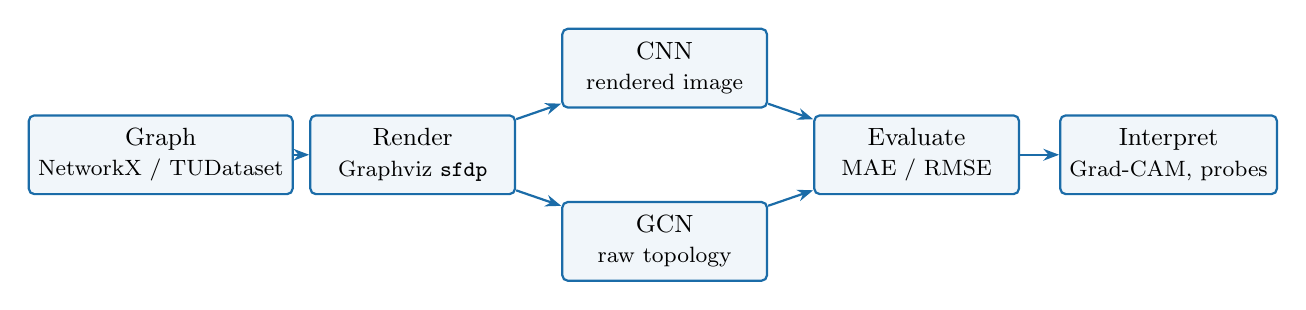
\begin{tikzpicture}[
    box/.style={draw=accent, thick, rounded corners=2pt, fill=accent!6, minimum height=10mm, minimum width=26mm, align=center, font=\small},
    arr/.style={-{Stealth[length=2mm]}, thick, accent}
]
\node[box] (graph) at (0,0) {Graph\\\footnotesize NetworkX / TUDataset};
\node[box] (render) at (3.2,0) {Render\\\footnotesize Graphviz \texttt{sfdp}};
\node[box] (cnn) at (6.4,1.1) {CNN\\\footnotesize rendered image};
\node[box] (gcn) at (6.4,-1.1) {GCN\\\footnotesize raw topology};
\node[box] (eval) at (9.6,0) {Evaluate\\\footnotesize MAE / RMSE};
\node[box] (interpret) at (12.8,0) {Interpret\\\footnotesize Grad-CAM, probes};

\draw[arr] (graph) -- (render);
\draw[arr] (render) -- (cnn);
\draw[arr] (render) -- (gcn);
\draw[arr] (cnn) -- (eval);
\draw[arr] (gcn) -- (eval);
\draw[arr] (eval) -- (interpret);
\end{tikzpicture}%
}
\caption{End-to-end Topolens pipeline. Every graph is rendered once and then scored two ways---visually by the CNN and natively by the GCN---so that the only thing separating the two model paths is the encoder, not the underlying data.}
\label{fig:pipeline_overview}
\end{figure}

Framing the project this way, as a controlled comparison rather than as a leaderboard exercise aimed purely at maximizing accuracy, matters for how the rest of this report should be read. It would have been easy to report a single headline accuracy number and stop there; the more useful contribution of a project like this lies in exposing the conditions under which that number can be trusted and the conditions under which it cannot. An image-based estimator that performs well only because of an accidental rendering convention is not obviously useful outside the narrow setting where that convention happens to hold, and a report that failed to check for this would risk overstating what has actually been demonstrated. This is why comparable weight is given in this report to the process of building the pipeline correctly (Sections~\ref{sec:background}--\ref{sec:results}) as to interrogating the resulting model's behavior before trusting it (Section~\ref{ch:interpretation}), rather than treating the interpretability analysis as an afterthought once the accuracy numbers were already in hand.

Concretely, this report makes the following contributions:
\begin{enumerate}[leftmargin=18pt, itemsep=3pt]
    \item A controlled, stratified benchmark of 2,500 synthetic graphs (5 generator families $\times$ 4 size tiers) plus 1,301 real-world held-out graphs (MUTAG, PROTEINS), rendered through a single documented, reproducible pipeline.
    \item A deliberately minimal-feature GCN baseline design that isolates topology-as-rendered-geometry from topology-as-raw-connectivity, so that the CNN-vs-GNN comparison is a controlled experiment rather than an incidental benchmark race.
    \item A multi-pronged interpretability suite---Grad-CAM, a causal node-size ablation validated with paired Wilcoxon tests, a layout-sensitivity probe, and a pixel-only baseline---applied jointly to the same trained model, rather than any single diagnostic taken in isolation.
    \item Two empirically substantiated findings treated as first-class results rather than footnotes: a quantified node-size rendering confound, and a fairness qualification on the baseline comparison, both of which materially change how the headline accuracy numbers should be read.
    \item An end-to-end validation of the offline findings against the actual deployed inference application, including out-of-style novel images the pipeline had never encountered in any form.
\end{enumerate}

By answering these questions, we demonstrate the strengths and major failure modes of image-based topology regression, qualifying the quantitative performance with a detailed analysis of shortcut learning. The remainder of this report is organized to build toward that answer step by step: Section~\ref{sec:background} formalizes the prediction task and the evaluation criteria; Section~\ref{sec:dataset} describes how the synthetic and real-world graph datasets were assembled; Section~\ref{sec:rendering} documents exactly how graphs are turned into images, since the rendering choices made there turn out to matter a great deal; Section~\ref{sec:model} and Section~\ref{sec:training} describe the CNN, the GCN baseline, and how both were trained; Section~\ref{sec:results} reports the headline quantitative comparison; Section~\ref{ch:interpretation} is where the Mechanism question is actually answered, through Grad-CAM, targeted probes, and statistical testing; and Sections~\ref{ch:discussion}--\ref{sec:conclusion} discuss what the combined evidence means, where it should not be over-trusted, and what a natural next iteration of this project would look like.

% ----------------------------------------------------------------------
% SECTION 2: RELATED WORK
% ----------------------------------------------------------------------
\section{Related Work}
\label{sec:relatedwork}
This section situates Topolens relative to three adjacent bodies of work: graph-native representation learning, graph drawing and visualization, and the study of shortcut learning in deep networks. None of these three areas directly addresses the specific question this report asks---estimating structural graph properties from a rendered image via an ordinary CNN---and that gap is itself part of the motivation described in Section~\ref{sec:introduction}.

\subsection{Graph-Native Representation Learning}
The dominant paradigm for learning from graph-structured data is message passing, in which a Graph Neural Network iteratively aggregates information from each node's neighborhood~[\ref{ref:gcn}]. This report's GCN baseline (Section~\ref{sec:model}) is a direct, minimal instance of this paradigm, implemented via PyTorch Geometric~[\ref{ref:pyg}]. Because GNNs operate on the graph itself rather than on any rendering of it, they are the natural benchmark against which a purely visual estimator should be measured, and the entire Competitiveness question posed in Section~\ref{sec:introduction} is framed as a comparison against this paradigm rather than against other visual baselines.

\subsection{Graph Drawing and Visual Graph Representations}
Separately, the graph drawing literature has long studied how to lay out a graph's nodes and edges in 2D space for human readability, with force-directed placement---in which nodes repel each other while edges act as springs---as one of the most widely used families of approach~[\ref{ref:fruchterman}]. Graphviz's \texttt{sfdp} engine~[\ref{ref:graphviz}], used throughout this report's rendering pipeline (Section~\ref{sec:rendering}), is a scalable implementation of this family. This literature is concerned with producing layouts that are readable to \emph{humans}; it does not ask whether a trained visual model can recover structural statistics from the resulting image, which is the question this report investigates instead.

\subsection{Shortcut Learning and Interpretability}
Deep networks are well documented to sometimes solve a task by exploiting incidental statistical regularities in the training data rather than the intended underlying signal, a phenomenon broadly termed shortcut learning~[\ref{ref:geirhos}]. The node-size rendering confound identified in Section~\ref{ch:interpretation} is a concrete instance of this general phenomenon, specific to the graph-rendering setting: because node radius is a deterministic function of vertex count in this pipeline (Section~\ref{sec:rendering}), it constitutes exactly the kind of spurious-but-predictive cue that shortcut learning describes. This report's use of Grad-CAM~[\ref{ref:gradcam}] and targeted causal ablation, rather than accuracy numbers alone, follows directly from taking that risk seriously rather than assuming it away.

\subsection{Positioning of This Work}
To the best of the author's knowledge, no prior work directly studies the specific setting examined here: training an ordinary CNN to regress structural graph statistics (vertex and edge counts) from a rendered image, benchmarked jointly against a graph-native GNN baseline and audited for rendering-specific shortcuts. This report should therefore be read as a controlled, exploratory case study bridging the three areas above, rather than as an incremental improvement on an established benchmark within any one of them.

% ----------------------------------------------------------------------
% SECTION 3: BACKGROUND & PROBLEM STATEMENT
% ----------------------------------------------------------------------
\section{Background \& Problem Statement}
\label{sec:background}

\subsection{Problem Statement}
The objective of this project is to solve the problem of graph topology regression from images. Specifically, given a single rendered image of a graph, the model must output two continuous values which are subsequently rounded to non-negative integers representing the predicted vertex count ($V$) and edge count ($E$).

Formally, let $G = (V, E)$ be a graph, and $I = \mathcal{R}(G)$ be its rendered image, where $\mathcal{R}$ is a rendering function mapping the topological structure to a 2D pixel space. The model $f(I)$ seeks to predict $y = [|V|, |E|]$. We benchmark this visual prediction pipeline against a graph-native Graph Convolutional Network (GCN) baseline $g(G)$ and a simple graph-statistic heuristic. A successful solution must achieve low Mean Absolute Error (MAE) and Root Mean Squared Error (RMSE) on both synthetic in-distribution test images and out-of-distribution real-world images from benchmark chemical and biological datasets.

The task is deliberately framed as regression rather than classification. Vertex and edge counts are unbounded, ordinally meaningful quantities (a graph with 40 nodes is topologically closer to one with 41 nodes than to one with 4), so collapsing them into discrete class buckets would throw away exactly the ordering information a useful estimator needs to preserve. MAE and RMSE are reported together rather than either alone because they answer different questions: MAE gives a robust, outlier-resistant sense of typical error, while RMSE's squaring penalizes the occasional catastrophic miss more heavily---and, as the failure-taxonomy results in Section~\ref{ch:interpretation} show, this project does produce a long tail of large misses on out-of-distribution graphs, so relying on MAE alone would understate how bad those failures are. Evaluating on both an in-distribution synthetic test split and an out-of-distribution real-world held-out split is likewise deliberate: a model that only works on graphs drawn from the same generator family it was trained on is of limited practical use, so the held-out MUTAG/PROTEINS split exists specifically to stress-test generalization beyond the synthetic distribution.

\subsection{Notation and Abbreviations}
\label{sec:notation}
For reference throughout the report, Table~\ref{tab:notation} summarizes the mathematical notation introduced above and used in later sections, and Table~\ref{tab:abbreviations} lists recurring abbreviations.

\begin{table}[htbp]
\centering
\caption{Mathematical Notation}
\label{tab:notation}
\begin{tabular}{ll}
\toprule
Symbol & Meaning \\
\midrule
$G = (V, E)$ & A graph with vertex set $V$ and edge set $E$ \\
$n$, $m$ & Number of vertices ($n = |V|$) and edges ($m = |E|$) of a graph \\
$I = \mathcal{R}(G)$ & Rendered image of graph $G$ under rendering function $\mathcal{R}$ \\
$f(I)$ & CNN model, mapping a rendered image to predicted $[|V|, |E|]$ \\
$g(G)$ & GCN model, mapping a graph directly to predicted $[|V|, |E|]$ \\
$x_v$ & Normalized-degree input feature of node $v$ in the GCN \\
$y_{\text{true}}$, $y_{\text{pred}}$ & Ground-truth and predicted regression targets \\
$p$ & Edge-inclusion probability (generator parameter) or statistical $p$-value, by context \\
$r$ & Pearson correlation coefficient \\
$R^2$ & Coefficient of determination \\
\bottomrule
\end{tabular}
\end{table}

\begin{table}[htbp]
\centering
\caption{Abbreviations}
\label{tab:abbreviations}
\begin{tabular}{ll}
\toprule
Abbreviation & Meaning \\
\midrule
CNN & Convolutional Neural Network \\
GNN & Graph Neural Network \\
GCN & Graph Convolutional Network \\
MAE & Mean Absolute Error \\
RMSE & Root Mean Squared Error \\
OOD & Out-of-Distribution \\
\texttt{sfdp} & Scalable Force-Directed Placement (Graphviz layout engine) \\
TUDataset & TU Dortmund graph benchmark collection \\
Grad-CAM & Gradient-weighted Class Activation Mapping \\
DPI & Dots Per Inch \\
\bottomrule
\end{tabular}
\end{table}

\subsection{Motivation: Personal Context}
This project began as a personal exploration of a question sitting at the intersection of computer vision and graph representation learning: whether a CNN operating purely on rendered images can recover structural properties that graph-native models compute directly from topology. The problem framing---inferring graph structure from images rather than from graph-native representations---was chosen deliberately as a research contrast rather than a practical workaround, motivated by the author's existing interest in computer vision. In practice, this meant that once the initial pipeline was working, additional time was spent specifically on the interpretability analysis in Section~\ref{ch:interpretation}---probing \emph{why} the model works rather than stopping at the headline accuracy numbers---since that question was of independent interest to the author beyond the core pipeline itself.

% ----------------------------------------------------------------------
% SECTION 3: DATASET DESCRIPTION
% ----------------------------------------------------------------------
\section{Dataset Description}
\label{sec:dataset}

\subsection{Synthetic Dataset Pool}
The primary training, validation, and testing dataset consists of 2,500 synthetic graphs generated via NetworkX~[\ref{ref:networkx}]. The dataset is stratified across 5 generator families crossed with 4 node-count tiers. Each cell in this generator $\times$ tier matrix contains exactly 125 graphs. The generator families and tiers were chosen deliberately rather than arbitrarily: each family instantiates a structurally distinct regime that a purely visual model might respond to very differently (uniformly random connectivity, scale-free hub formation, small-world clustering, strict tree hierarchies, and saturated density), while the four tiers ensure the model is exposed to a wide range of absolute node/edge counts rather than a narrow band where a crude heuristic could trivially succeed. Stratifying across both axes, rather than sampling freely, guarantees that no single tier or family dominates the training signal and that later breakdown analyses (Section~\ref{sec:results}) are comparing like-for-like sample sizes.
The node range for each tier is defined as follows:
\begin{itemize}
    \item \textbf{tiny:} 5--10 nodes
    \item \textbf{small:} 10--25 nodes
    \item \textbf{medium:} 25--50 nodes
    \item \textbf{large:} 50--100 nodes
\end{itemize}

The 5 generator families and their specific parameters from \texttt{config.yaml} are:
\begin{enumerate}
    \item \textbf{Erdős--Rényi (\texttt{erdos\_renyi})~[\ref{ref:erdosrenyi}]:} Random graphs with edge probability parameter $p \in \{0.05, 0.1, 0.2, 0.3\}$. Every edge is included independently at random, giving a structurally ``featureless'' baseline topology with no hubs and no clustering beyond what chance produces.
    \item \textbf{Barabási--Albert (\texttt{barabasi\_albert})~[\ref{ref:barabasialbert}]:} Preferential attachment scale-free graphs with parameter $m \in \{1, 2, 3, 5\}$ representing the number of edges to attach from a new node to existing nodes. This family produces hub-and-spoke structures, which render visually as a small number of highly connected nodes surrounded by sparser satellites---a distinct visual signature from Erdős--Rényi graphs of the same size.
    \item \textbf{Watts--Strogatz (\texttt{watts\_strogatz})~[\ref{ref:wattsstrogatz}]:} Small-world graphs with neighborhood size parameter $k \in \{4, 6\}$ and rewiring probability $p \in \{0.1, 0.3\}$. These graphs combine local clustering with a few long-range shortcuts, giving a ring-like visual layout punctuated by occasional cross-connections.
    \item \textbf{Random Trees (\texttt{random\_tree}):} Graph trees generated randomly using a deterministic spacing generator. Trees are the sparsest possible connected topology (exactly $n-1$ edges), included specifically to test the model at the low-density extreme.
    \item \textbf{Dense Erdős--Rényi variants (\texttt{dense}):} Denser random graphs with edge probability parameter $p \in \{0.6, 0.8, 0.95\}$. These sit at the opposite density extreme from the trees and, as later chapters show, turn out to be the \emph{easiest} case for the CNN rather than the hardest, which is itself a notable finding rather than an expected one.
\end{enumerate}

Each graph's render and layout seed is derived deterministically from its \texttt{graph\_id} via SHA-256, ensuring bit-for-bit reproducibility. The synthetic pool is split into train (70\%, 1,750 graphs), validation (15\%, 375 graphs), and test (15\%, 375 graphs) splits, stratified by generator type, using seed 42.

\begin{figure}[htbp]
    \centering
    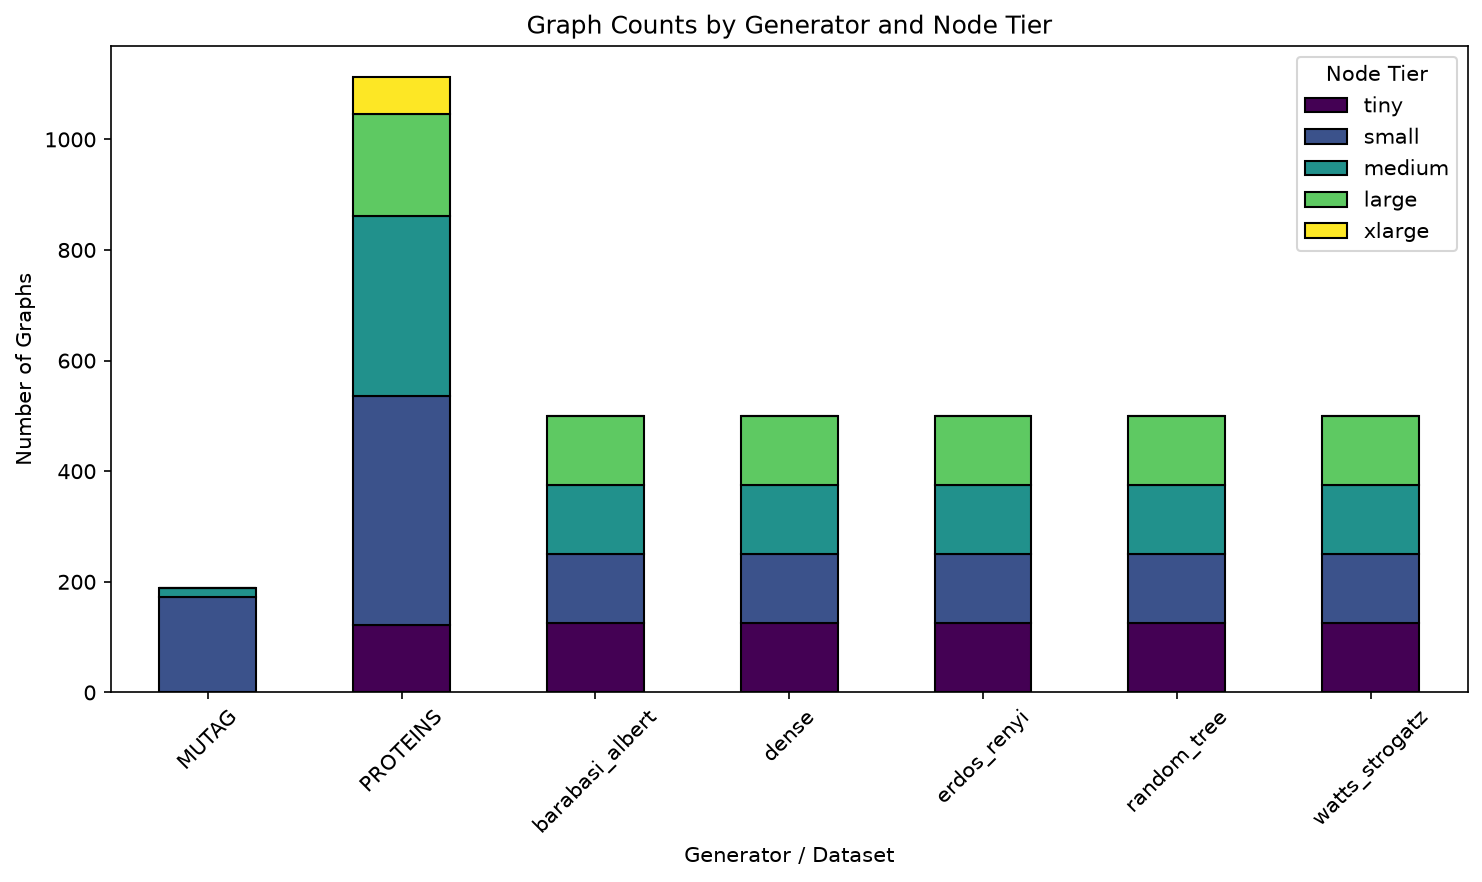
\includegraphics[width=0.6\textwidth, height=0.75\textheight, keepaspectratio]{../figures/graph_counts_by_tier.png}
    \caption{Distribution of graph counts across the synthetic size tiers.}
    \label{fig:graph_counts_by_tier}
\end{figure}
\FloatBarrier

\subsection{Held-out Real-World Dataset}
To test out-of-distribution generalization, we incorporate 1,301 real-world graphs loaded via PyTorch Geometric's \texttt{TUDataset}~[\ref{ref:tudataset}]. These benchmarks were chosen because they are standard, widely-used graph-learning datasets from two different application domains (chemistry and biology), which lets us check whether anything the model learns from synthetic generator graphs transfers to structurally organic, human- or nature-produced topologies. The datasets are stripped of chemical/biological labels to expose only raw topology:
\begin{itemize}
    \item \textbf{MUTAG (188 graphs)~[\ref{ref:mutag}]:} A dataset of mutagenic aromatic and heteroaromatic nitro compounds. They are small and structurally homogeneous.
    \item \textbf{PROTEINS (1,113 graphs)~[\ref{ref:proteins}]:} Contact maps representing secondary structure elements. They have a broad size distribution, spanning 4 to 620 nodes. Crucially, 67 of the PROTEINS graphs exceed the training ceiling of 100 nodes, serving as a severe size generalization test.
\end{itemize}
The held-out set was never seen during training or model selection, so any accuracy reported on it in Section~\ref{sec:results} reflects genuine generalization rather than memorization of the training distribution.

\subsection{Split and Crosstabulation Statistics}
The exact per-split, per-tier, and per-generator counts pulled directly from the processed dataset CSVs are presented in Tables~\ref{tab:train_split_counts}, \ref{tab:val_split_counts}, \ref{tab:test_split_counts}, and \ref{tab:held_out_split_counts}. These tables exist primarily as a stratification audit: because the splits are meant to be balanced across generator family and size tier, listing the raw counts lets a reader verify directly that no split is accidentally skewed toward one family or tier, which would otherwise silently bias the reported metrics. The corresponding structural distributions are visualized in Figure~\ref{fig:distributions_overall} and Figure~\ref{fig:distributions_by_generator}.

\begin{figure}[htbp]
    \centering
    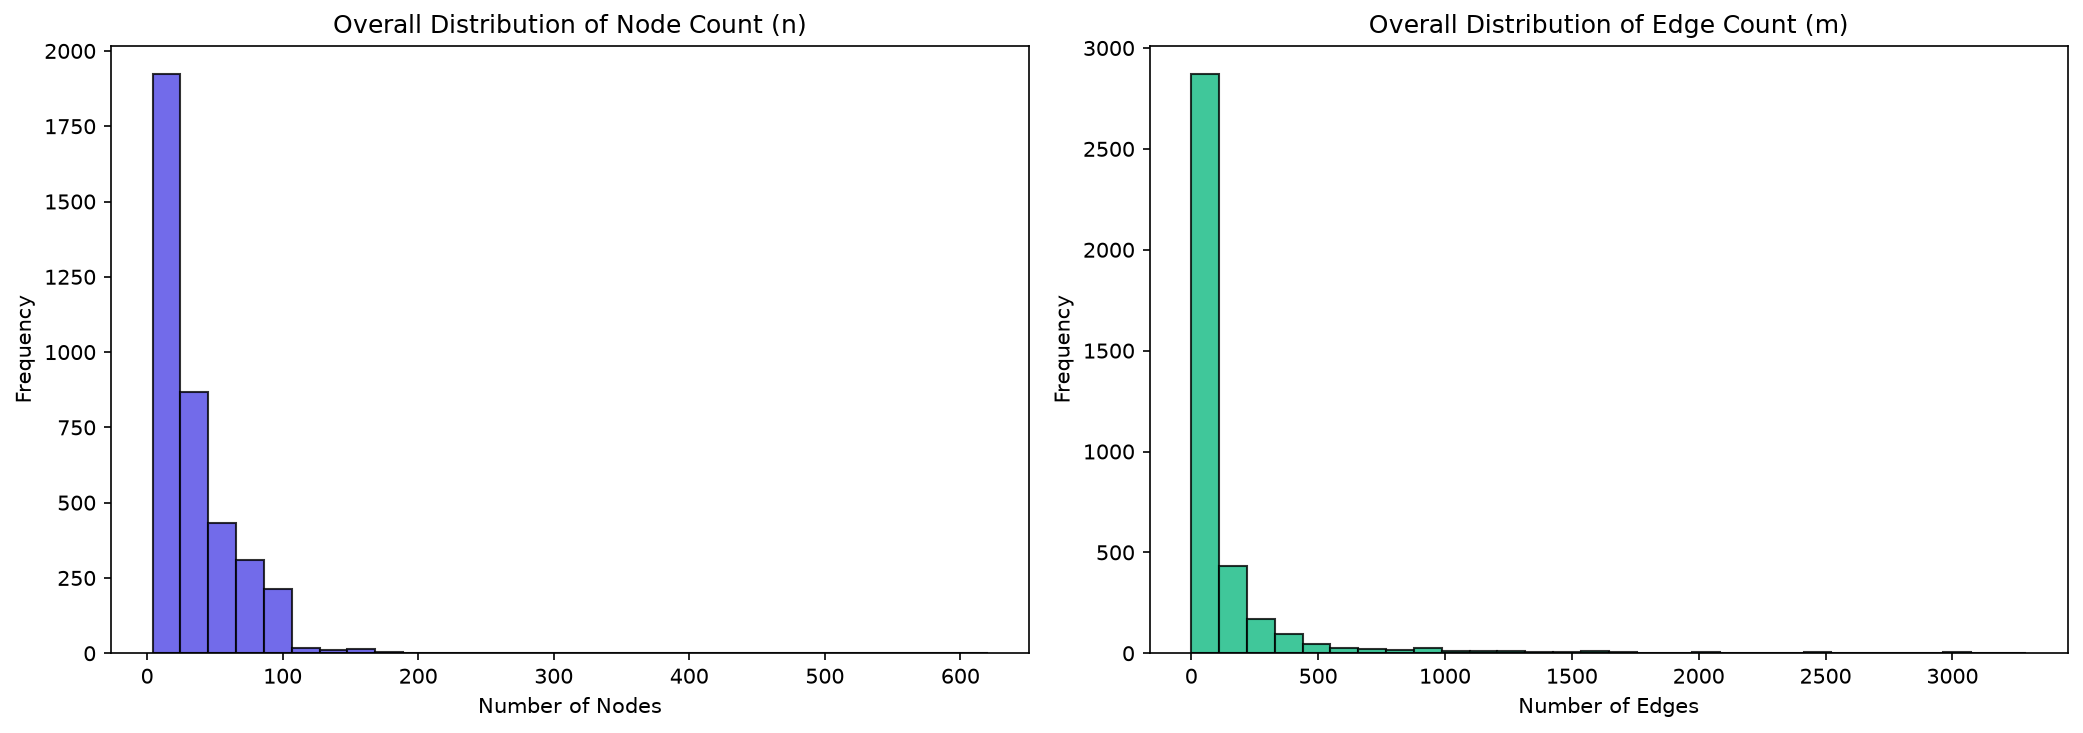
\includegraphics[width=0.6\textwidth, height=0.75\textheight, keepaspectratio]{../figures/node_edge_distributions_overall.png}
    \caption{Overall node and edge count distributions across the dataset.}
    \label{fig:distributions_overall}
\end{figure}
\FloatBarrier

\begin{figure}[htbp]
    \centering
    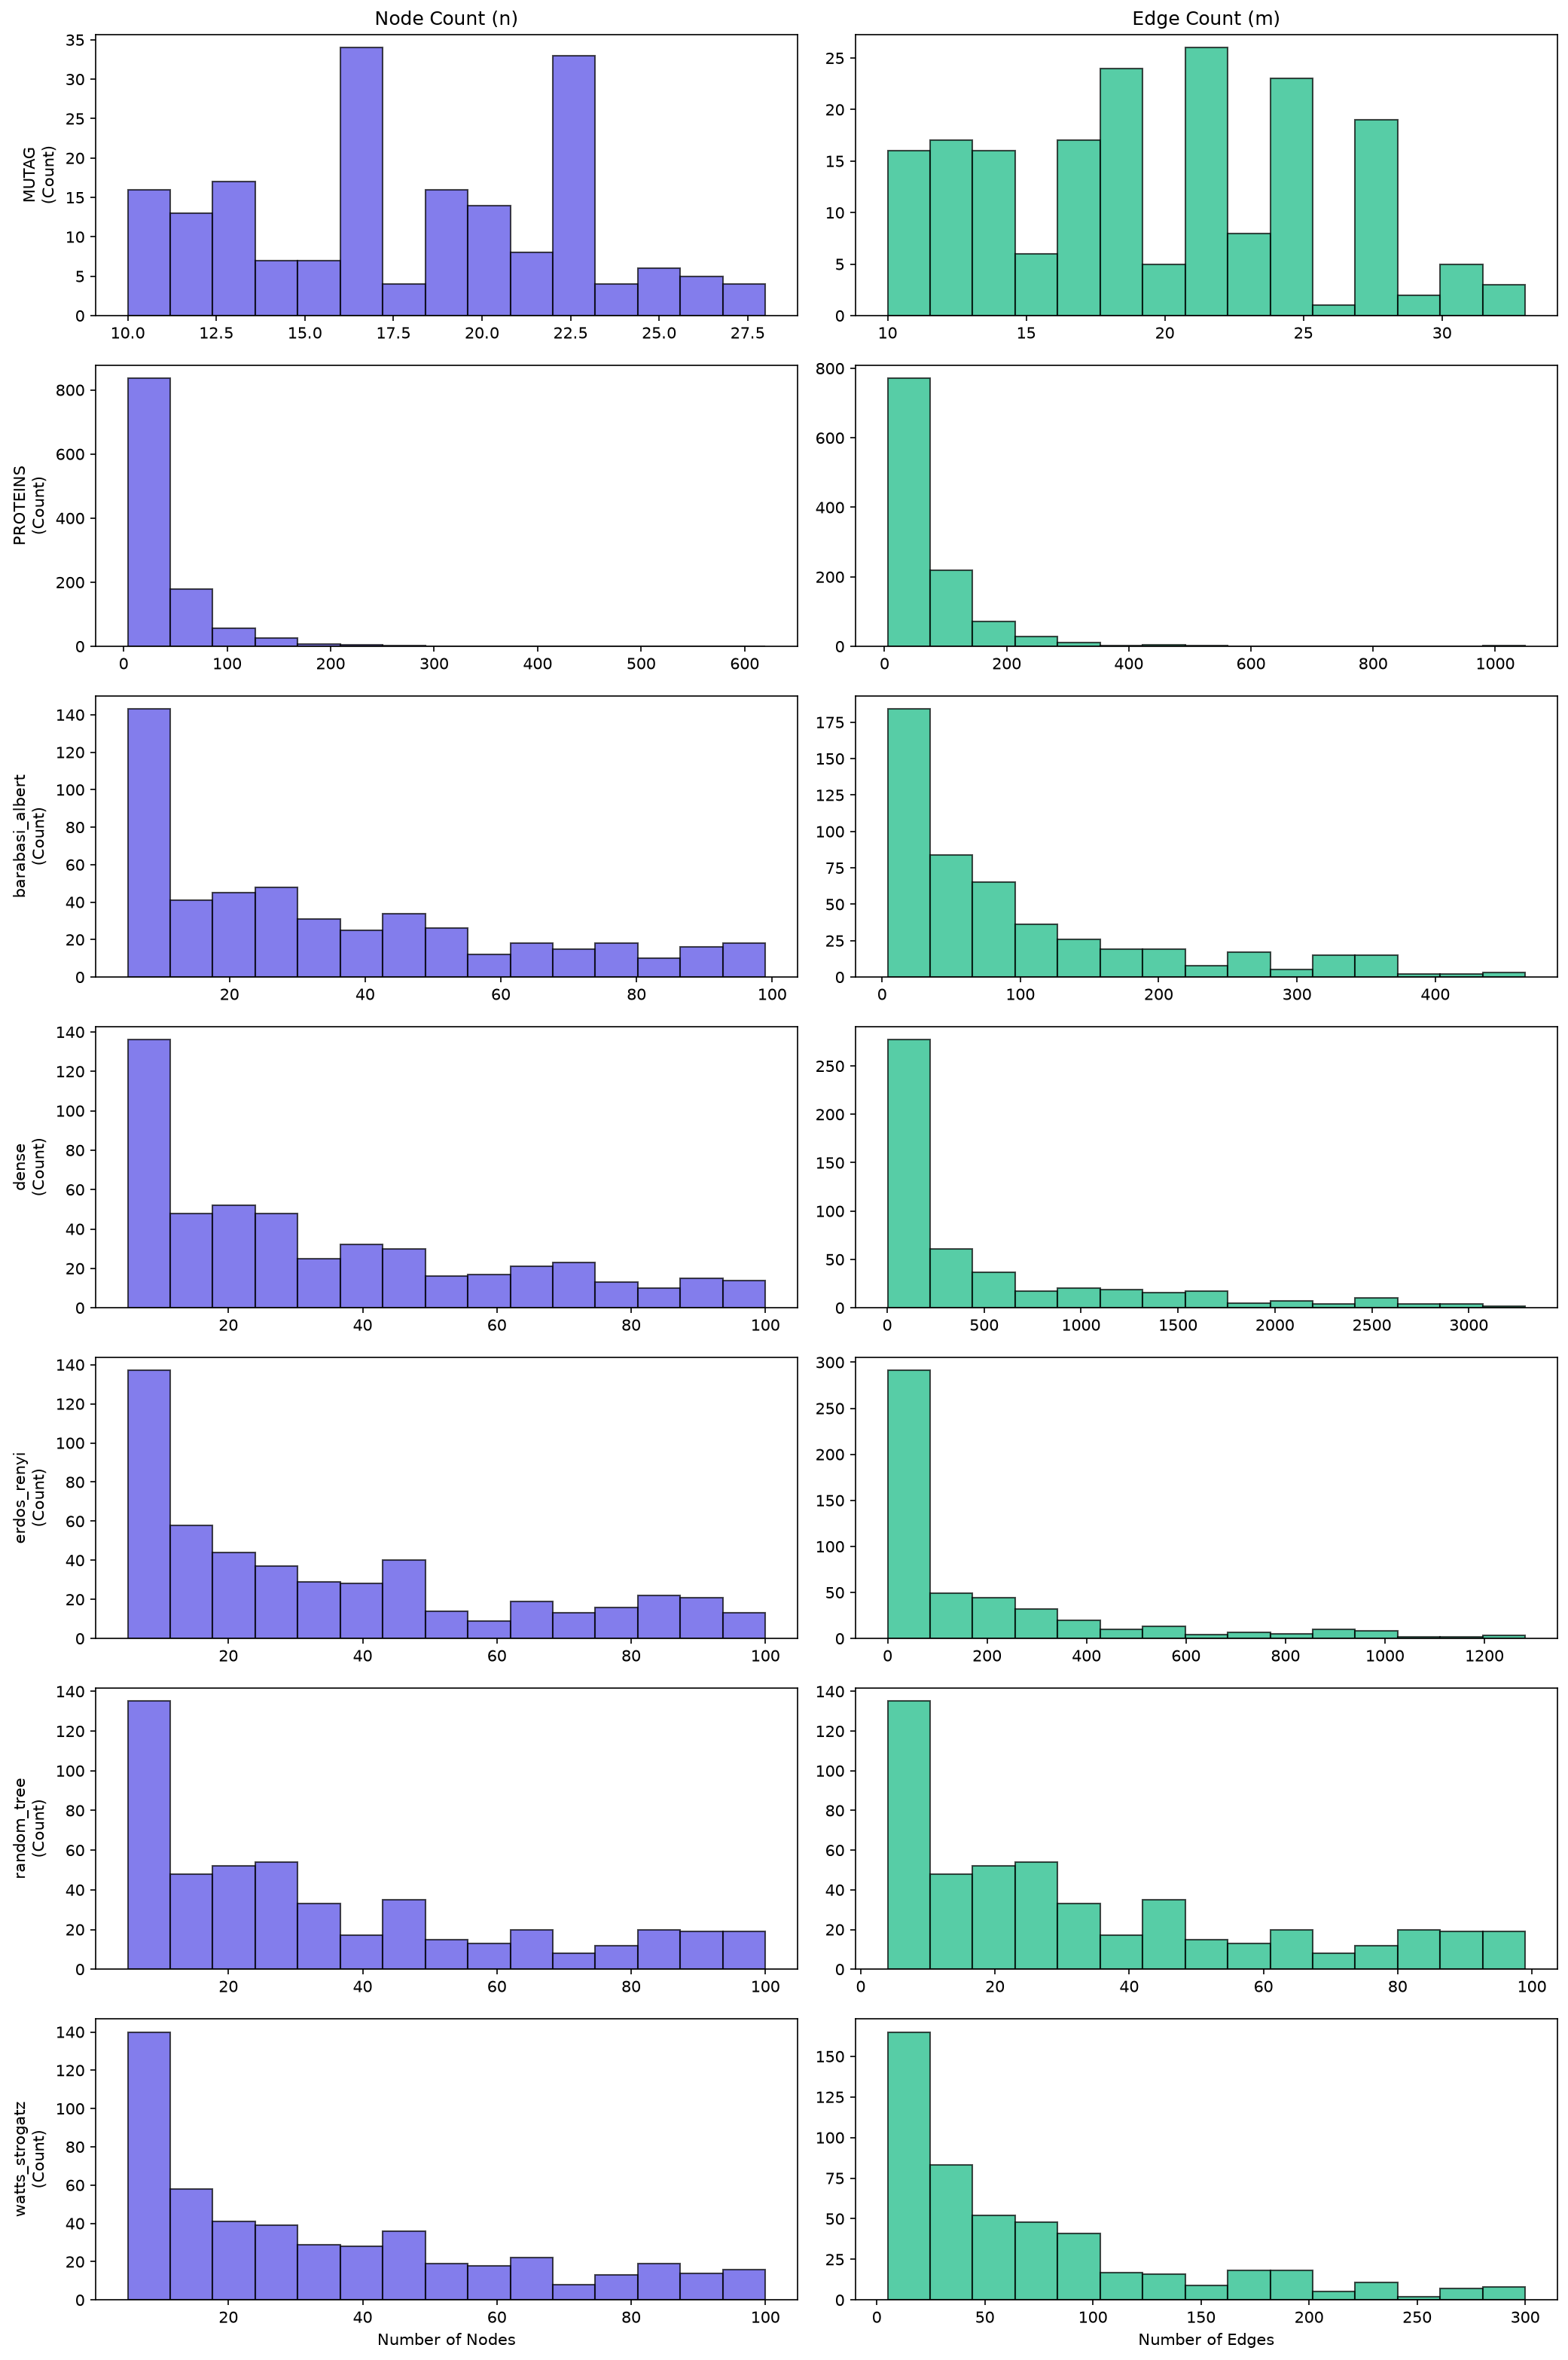
\includegraphics[width=0.9\textwidth, height=0.75\textheight, keepaspectratio]{../figures/node_edge_distributions_by_generator.png}
    \caption{Node and edge distributions broken down by generator family.}
    \label{fig:distributions_by_generator}
\end{figure}
\FloatBarrier

\begin{table}[htbp]
\centering
\caption{Train Split Sample Counts by Generator and Tier ($n=1,750$)}
\label{tab:train_split_counts}
\begin{tabular}{lccccc}
\toprule
Generator & Tiny (5--10) & Small (10--25) & Medium (25--50) & Large (50--100) & Total \\
\midrule
barabasi\_albert & 89 & 92 & 92 & 77 & 350 \\
dense & 88 & 95 & 83 & 84 & 350 \\
erdos\_renyi & 82 & 83 & 94 & 91 & 350 \\
random\_tree & 92 & 86 & 89 & 83 & 350 \\
watts\_strogatz & 91 & 89 & 88 & 82 & 350 \\
\midrule
Total & 442 & 445 & 446 & 417 & 1,750 \\
\bottomrule
\end{tabular}
\end{table}

\begin{table}[htbp]
\centering
\caption{Validation Split Sample Counts by Generator and Tier ($n=375$)}
\label{tab:val_split_counts}
\begin{tabular}{lccccc}
\toprule
Generator & Tiny (5--10) & Small (10--25) & Medium (25--50) & Large (50--100) & Total \\
\midrule
barabasi\_albert & 22 & 13 & 16 & 24 & 75 \\
dense & 17 & 21 & 18 & 19 & 75 \\
erdos\_renyi & 23 & 17 & 14 & 21 & 75 \\
random\_tree & 15 & 22 & 18 & 20 & 75 \\
watts\_strogatz & 20 & 14 & 21 & 20 & 75 \\
\midrule
Total & 97 & 87 & 87 & 104 & 375 \\
\bottomrule
\end{tabular}
\end{table}

\begin{table}[htbp]
\centering
\caption{Test Split Sample Counts by Generator and Tier ($n=375$)}
\label{tab:test_split_counts}
\begin{tabular}{lccccc}
\toprule
Generator & Tiny (5--10) & Small (10--25) & Medium (25--50) & Large (50--100) & Total \\
\midrule
barabasi\_albert & 14 & 20 & 17 & 24 & 75 \\
dense & 20 & 9 & 24 & 22 & 75 \\
erdos\_renyi & 20 & 25 & 17 & 13 & 75 \\
random\_tree & 18 & 17 & 18 & 22 & 75 \\
watts\_strogatz & 14 & 22 & 16 & 23 & 75 \\
\midrule
Total & 86 & 93 & 92 & 104 & 375 \\
\bottomrule
\end{tabular}
\end{table}

\begin{table}[htbp]
\centering
\caption{Held-out (Real-world) Split Sample Counts by Source and Tier ($n=1,301$)}
\label{tab:held_out_split_counts}
\small
\begin{tabular}{lcccccc}
\toprule
Source & Tiny (5--10) & Small (10--25) & Medium (25--50) & Large (50--100) & XLarge ($>100$) & Total \\
\midrule
MUTAG & 0 & 173 & 15 & 0 & 0 & 188 \\
PROTEINS & 122 & 414 & 326 & 184 & 67 & 1,113 \\
\midrule
Total & 122 & 587 & 341 & 184 & 67 & 1,301 \\
\bottomrule
\end{tabular}
\end{table}

% ----------------------------------------------------------------------
% SECTION 4: RENDERING PIPELINE
% ----------------------------------------------------------------------
\section{Rendering Pipeline}
\label{sec:rendering}
Each graph is rendered to a $224 \times 224$ px PNG image at 100 DPI. This resolution was chosen as a standard, well-supported CNN input size that keeps training computationally tractable on the available hardware (Section~\ref{sec:training}) while still leaving enough pixel detail to distinguish individual nodes in the \texttt{large} tier. The layout is determined using a deterministic three-stage fallback chain:
\begin{equation*}
\text{pygraphviz sfdp} \longrightarrow \text{pydot sfdp} \longrightarrow \text{NetworkX spring layout}
\end{equation*}
This chain exists for robustness rather than by design intent: \texttt{pygraphviz} is the preferred binding to Graphviz~[\ref{ref:graphviz}]'s force-directed \texttt{sfdp} layout engine, but it depends on a system-level Graphviz installation that is not guaranteed to be present on every machine the pipeline might run on (including, potentially, a grader's or reviewer's environment); \texttt{pydot} is a lighter-weight fallback that still calls out to the same underlying Graphviz binary, and NetworkX's pure-Python spring layout is a last resort that requires no external dependency at all. In practice, all 3,801 rendered images (synthetic and real) successfully resolved through Graphviz \texttt{sfdp} (verified via the \texttt{layout\_algorithm} field in \texttt{labels\_processed.csv}), so the fallback tiers were never actually exercised---but their presence is what makes the rendering step reproducible across environments rather than silently failing. Figure~\ref{fig:sample_render_grid} displays a representative sample render grid.

\begin{figure}[htbp]
    \centering
    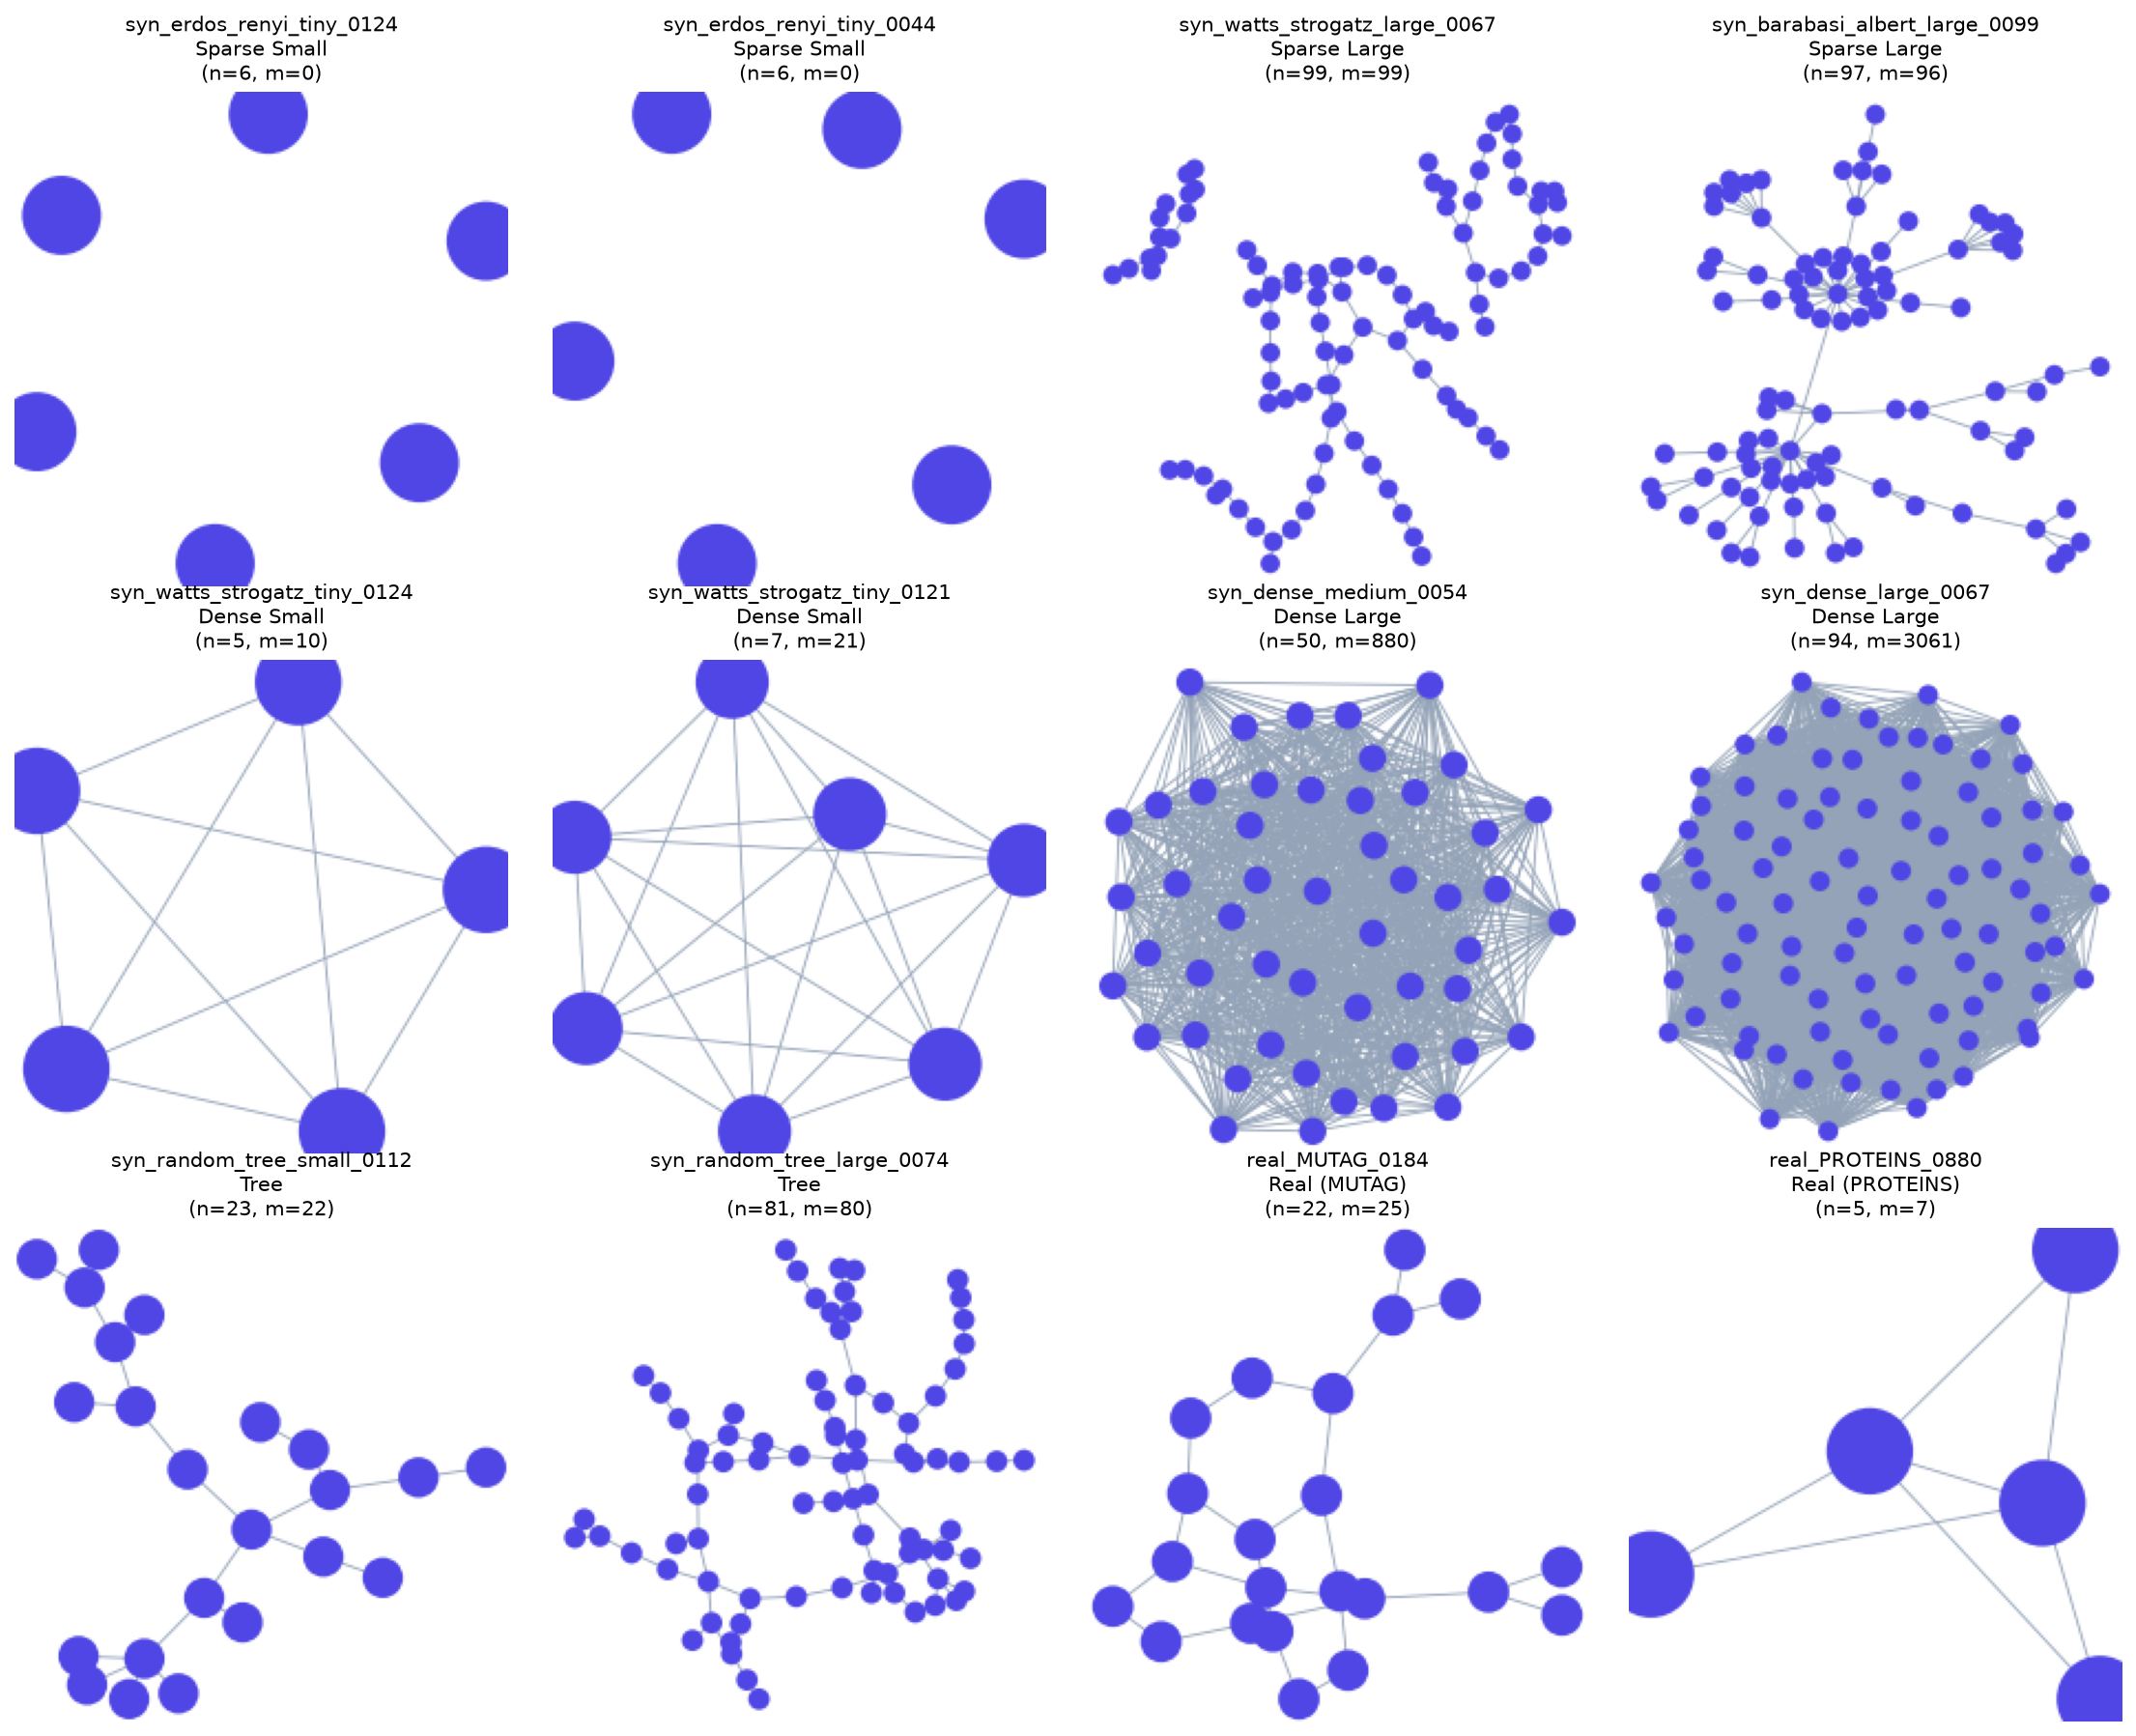
\includegraphics[width=0.8\textwidth, height=0.75\textheight, keepaspectratio]{../figures/sample_render_grid.png}
    \caption{Sample rendered images from the dataset showcasing different topologies.}
    \label{fig:sample_render_grid}
\end{figure}
\FloatBarrier

The visual style is defined by a solid white background, uniform node coloring (dark blue/purple), and fixed thin edges (width 0.6). Crucially, the node radius scales dynamically based on the vertex count $n$:
\begin{equation}
\text{radius} = \max\left(15, \frac{4000}{n}\right)
\label{eq:node_radius}
\end{equation}
This formula exists to solve a real rendering problem: at fixed node size, a 100-node graph packed into a $224\times224$ image becomes a solid blob of overlapping circles with no visible internal structure, which would make the image useless to both the CNN and a human viewer. Shrinking nodes as $n$ grows keeps the rendered graph visually legible across the full size range. However, this inverse size scaling introduces a significant confound: the model can potentially cheat by regressing the count directly from the physical size of the rendered nodes rather than counting individual nodes---since node radius and vertex count are, by construction, related by a fixed deterministic formula, a model does not need to understand topology at all to exploit it. This tension between legibility and confound-avoidance was recognized at design time and is analyzed empirically in Section~\ref{ch:interpretation}, where it turns out to be a real and statistically significant effect rather than a hypothetical one.

% ----------------------------------------------------------------------
% SECTION 5: MODEL ARCHITECTURE
% ----------------------------------------------------------------------
\section{Model Architecture}
\label{sec:model}

\subsection{Custom CNN Regressor (\texttt{CustomCNNRegressor})}
The visual model is a custom deep convolutional neural network consisting of 4 convolutional blocks followed by a fully-connected regression head. The depth and channel width were chosen to match the scale of the problem: with only 2,500 synthetic training graphs, a very deep or very wide backbone (e.g. a full ResNet) would be prone to overfitting, while four blocks give enough receptive-field growth to see the whole $224\times224$ image by the final layer without requiring a dataset an order of magnitude larger to train reliably.
Each convolutional block contains:
\begin{enumerate}
    \item $3 \times 3$ Convolution (stride 1, padding 1)
    \item 1D Batch Normalization
    \item ReLU Activation
    \item $2 \times 2$ Max-Pooling (stride 2)
\end{enumerate}
The channel progression through the blocks is $3 \rightarrow 32 \rightarrow 64 \rightarrow 128 \rightarrow 256$, following the common convention of doubling channel width each time spatial resolution is halved, so that the total amount of information the network can represent stays roughly balanced across depth. Following the final block, the feature map is reduced using Global Adaptive Average Pooling to a size of $256 \times 1 \times 1$, rather than flattening and feeding a large feature vector into the regression head; average pooling was chosen specifically because vertex and edge counts should not depend on \emph{where} in the image a node cluster happens to sit, and average pooling discards that positional information by construction while a flattened layer would not. The regression head contains:
\begin{equation*}
\text{Linear}(256 \rightarrow 128) \rightarrow \text{ReLU} \rightarrow \text{Dropout}(0.2) \rightarrow \text{Linear}(128 \rightarrow 2)
\end{equation*}
producing both the vertex-count and edge-count predictions from a single shared trunk, with dropout included specifically to regularize this small-dataset regime.

\subsection{GCN Baseline (\texttt{GraphCountGCN})}
The graph-native baseline consists of 3 Graph Convolutional Network~[\ref{ref:gcn}] layers (\texttt{GCNConv}, implemented via PyTorch Geometric~[\ref{ref:pyg}]) with progression: $1 \rightarrow 64 \rightarrow 64 \rightarrow 64$.
Each layer is followed by Batch Normalization and a ReLU activation. The node embeddings are pooled globally using a mean-pooling layer (\texttt{global\_mean\_pool}) and fed through a fully-connected regression head identical in shape to the CNN's ($64 \rightarrow 128 \rightarrow \text{ReLU} \rightarrow \text{Dropout}(0.2) \rightarrow \text{Linear}(128 \rightarrow 2)$); keeping the two regression heads identical was a deliberate fairness choice, so that any performance gap between the two models reflects the encoder (convolution-on-pixels vs. message-passing-on-topology) rather than a difference in how predictions are ultimately produced.
Crucially, the only input feature provided to each node is its normalized degree:
\begin{equation*}
x_v = \frac{\text{deg}(v)}{\max_{u \in V} \text{deg}(u)}
\end{equation*}
This GCN represents a minimal topological learner with a highly restricted feature budget---no node identity, no positional encoding, no coordinates, nothing but a single scalar per node. This was a deliberate design choice to isolate the comparison to \emph{topology alone} versus \emph{topology as rendered geometry}, rather than letting the GCN implicitly recover spatial information the CNN also has access to. It is also, as discussed in Section~\ref{ch:discussion} and Section~\ref{sec:limitations}, the single biggest caveat on the headline CNN-vs-GCN comparison, since a GCN given richer features would likely close some of the gap.

\subsection{Graph-Statistic Baseline}
The heuristic baseline represents a non-learned control: a sanity floor that any trained model should be expected to beat, and a useful reference point for how much of the task is ``solvable'' by simple counting rules alone rather than requiring learning at all. For vertices, it returns the true count (oracle). For edges, it computes the estimate:
\begin{equation*}
E_{\text{pred}} = \text{mean\_density\_per\_generator} \times \frac{n(n-1)}{2}
\end{equation*}
where the per-generator mean densities are computed on the training set. Because this heuristic assumes every graph of a given generator type shares that generator's average density, it should do reasonably well on graphs close to the population mean and poorly on outliers---a prediction borne out by the results in Section~\ref{sec:results}.

\subsection{Log Target Transformation}
Both continuous regression targets are transformed during training using:
\begin{equation*}
y_{\text{train}} = \log(y_{\text{true}} + 1)
\end{equation*}
This transformation matters because the raw target distribution is extremely right-skewed: edge counts in the training data range from 5 up to 1,049, so a model trained directly on raw counts would be dominated by loss contributions from the handful of large, dense graphs, at the expense of learning to distinguish, say, a 6-node graph from an 8-node one. The log transform compresses that dynamic range so gradient magnitudes stay comparable across small and large graphs alike. At inference, predictions are back-transformed via $\exp(y_{\text{pred}}) - 1$, rounded to the nearest integer, and clamped at 0 (since a negative vertex or edge count is not meaningful).

\subsection{Model Cards}
\label{sec:modelcards}
Table~\ref{tab:modelcard} summarizes both models in a single, scannable reference, in the spirit of standard model-reporting practice. Parameter counts are analytically derived from the layer-by-layer architecture described above (not measured from a saved checkpoint) and are reported as approximate, rounded figures rather than exact values.

\begin{table}[htbp]
\centering
\caption{Model Cards: CNN Regressor vs. GCN Baseline}
\label{tab:modelcard}
\small
\begin{tabular}{p{2.4cm}p{5.4cm}p{5.4cm}}
\toprule
Field & CNN Regressor (\texttt{CustomCNNRegressor}) & GCN Baseline (\texttt{GraphCountGCN}) \\
\midrule
Architecture & 4 conv blocks (Conv--BN--ReLU--MaxPool), $3\to32\to64\to128\to256$ channels, global average pool, FC head & 3 \texttt{GCNConv} layers with BN--ReLU, $1\to64\to64\to64$ channels, global mean pool, FC head \\
Parameters (approx.) & $\sim$423K & $\sim$17K \\
Input & $224\times224$ RGB rendered graph image & Graph with 1-dimensional normalized-degree node feature \\
Output & $[\hat{V}, \hat{E}]$ (vertex count, edge count) & $[\hat{V}, \hat{E}]$ (vertex count, edge count) \\
Training data & 1,750 synthetic training graphs (Section~\ref{sec:dataset}), rendered images only & Same 1,750 graphs, used as raw topology (no rendering) \\
Training regime & Adam, lr $=10^{-3}$, 30 epochs, batch size 32, log-MSE loss (Section~\ref{sec:training}) & Identical optimizer, schedule, and loss as the CNN \\
Intended use & Estimating vertex/edge counts from images of graphs rendered in a similar style (Graphviz \texttt{sfdp}, $\le$100 nodes) & Estimating vertex/edge counts from raw topology when it is directly available \\
Out-of-scope use & Graphs rendered in unfamiliar styles, graphs exceeding $\sim$100 nodes, or non-graph images (Section~\ref{sec:limitations}) & Any setting requiring richer structural reasoning than a single degree feature can support \\
Primary known limitation & Accuracy is partly attributable to a node-size rendering confound (Section~\ref{ch:interpretation}), not pure topological understanding & Deliberately minimal feature budget likely understates what GNNs can achieve on this task (Section~\ref{sec:limitations}) \\
\bottomrule
\end{tabular}
\end{table}

% ----------------------------------------------------------------------
% SECTION 6: TRAINING SETUP
% ----------------------------------------------------------------------
\section{Training Setup}
\label{sec:training}
Both models were trained using PyTorch~[\ref{ref:pytorch}] on a Google Colab environment with a T4 GPU, since the local development machine's CPU-only setup made full training runs impractical within the project's one-week timeline. The hyperparameters sourced from \texttt{config.yaml} are:
\begin{itemize}
    \item \textbf{Optimizer:} Adam~[\ref{ref:adam}] (learning rate = 0.001)
    \item \textbf{Loss Function:} Mean Squared Error (MSE) on the log-transformed targets
    \item \textbf{Batch Size:} 32
    \item \textbf{Epochs:} 30
    \item \textbf{Reproducibility:} Random seeds fixed at 42 for split generation and initialization
\end{itemize}
These are standard, widely-used defaults for small-to-medium image and graph regression tasks rather than the result of an extensive hyperparameter search; given the project's timeline, the priority was a stable, well-understood configuration over marginal tuning gains, and Adam with a $10^{-3}$ learning rate is a reasonable starting point for both a CNN and a GCN of this size. The best checkpoints were saved based on validation loss rather than the final epoch weights, which protects against reporting a model that has started to overfit the training set in its last few epochs. A retraining run revealed a GPU/cuDNN non-determinism effect, shifting test-split overall vertex MAE from 4.5 to 3.2 between otherwise identical runs; this is reported openly here (and revisited in the Limitations chapter) because it means the headline metrics in Section~\ref{sec:results} should be read as one draw from a distribution of plausible outcomes for this configuration, not as an exactly reproducible constant.

% ----------------------------------------------------------------------
% SECTION 7: RESULTS
% ----------------------------------------------------------------------
\section{Results}
\label{sec:results}

\subsection{Baseline Comparison}
The quantitative comparison results on the Test and Held-out splits are presented in Table~\ref{tab:baseline_comparison}. The CNN outperforms the GCN baseline on every single metric, achieving a 4--6$\times$ lower error on the synthetic split and a 2$\times$ lower error on the real held-out split. It also significantly outperforms the density heuristic. In practical terms, a vertex MAE of 3.20 on the synthetic test split means the CNN's typical prediction is within three nodes of the true count across graphs ranging from 5 to 100 nodes---a small error relative to the scale of the task, though as later chapters show, that error grows substantially on the largest and most out-of-distribution graphs rather than staying uniform. The GCN's much larger errors are consistent with the deliberately minimal, degree-only feature set described in Section~\ref{sec:model}: with no richer structural signal to draw on, it has comparatively little to work with beyond local connectivity patterns.

\begin{table}[htbp]
\centering
\caption{Baseline Comparison Metrics on Test and Held-out Splits}
\label{tab:baseline_comparison}
\begin{tabular}{lllccc}
\toprule
Split & Target & Metric & CNN & GCN & Graph-statistic \\
\midrule
\textbf{Test (Synthetic)} & Vertices & MAE & 3.20 & 19.05 & 0.00\textsuperscript{*} \\
& Vertices & RMSE & 6.08 & 26.61 & 0.00\textsuperscript{*} \\
& Edges & MAE & 25.39 & 148.98 & 120.53 \\
& Edges & RMSE & 81.75 & 391.67 & 233.51 \\
\midrule
\textbf{Held-out (Real)} & Vertices & MAE & 10.62 & 21.15 & 0.00\textsuperscript{*} \\
& Vertices & RMSE & 31.30 & 44.09 & 0.00\textsuperscript{*} \\
& Edges & MAE & 28.03 & 56.84 & 363.65 \\
& Edges & RMSE & 67.72 & 92.82 & 2155.29 \\
\bottomrule
\end{tabular}
\begin{flushleft}
\small \textsuperscript{*} The graph-statistic baseline's 0.0 vertex MAE is structurally trivial (it returns the true node count directly). Only its edge heuristic is a genuine prediction.
\end{flushleft}
\end{table}

\subsection{Detailed Breakdown Reports}
Detailed performance breakdowns by generator type (test split), source dataset (held-out split), and density bucket (held-out split) are shown in Tables~\ref{tab:generator_breakdown}, \ref{tab:dataset_breakdown}, and \ref{tab:density_breakdown}. These breakdowns exist to check whether the aggregate numbers in Table~\ref{tab:baseline_comparison} are representative or are instead being carried by one easy subgroup while others perform far worse. Predictions on the test split are visually compared in Figure~\ref{fig:vertices_scatter_test} and Figure~\ref{fig:edges_scatter_test}, and predictions on the held-out split are analyzed in Figure~\ref{fig:vertices_scatter_held_out} and Figure~\ref{fig:edges_scatter_held_out}.

\begin{figure}[htbp]
    \centering
    \begin{subfigure}[b]{0.45\textwidth}
        \centering
        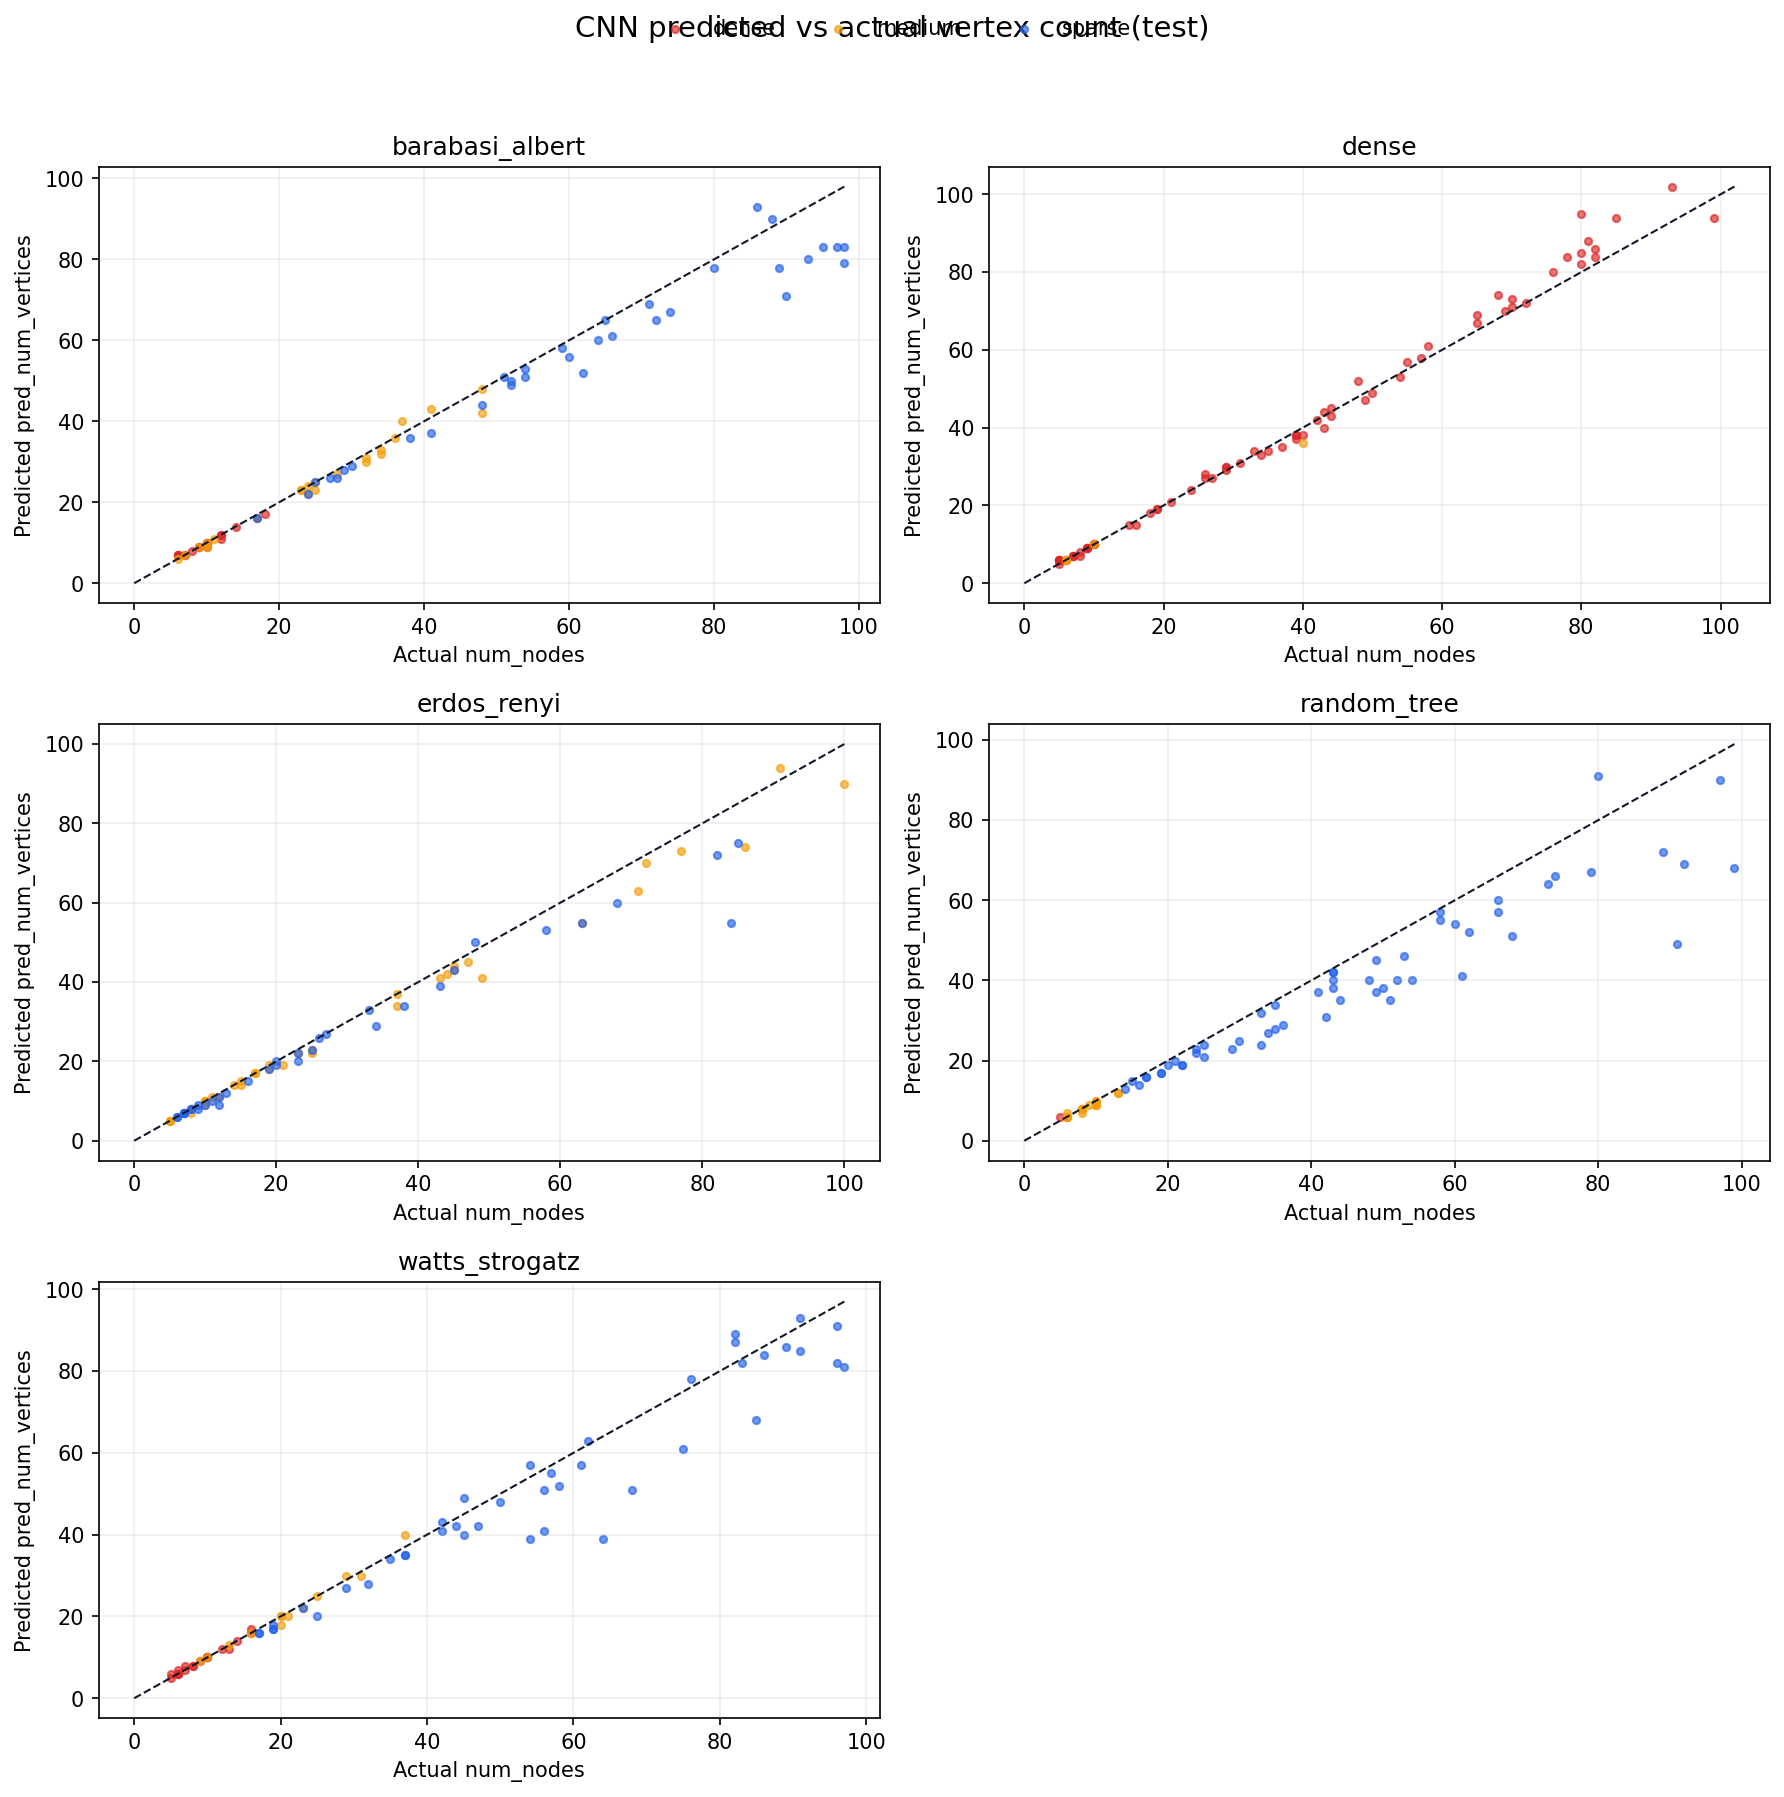
\includegraphics[width=\textwidth, height=0.75\textheight, keepaspectratio]{../figures/cnn_pred_num_vertices_scatter_test.png}
        \caption{Vertex count predictions (test split).}
        \label{fig:vertices_scatter_test}
    \end{subfigure}
    \hfill
    \begin{subfigure}[b]{0.45\textwidth}
        \centering
        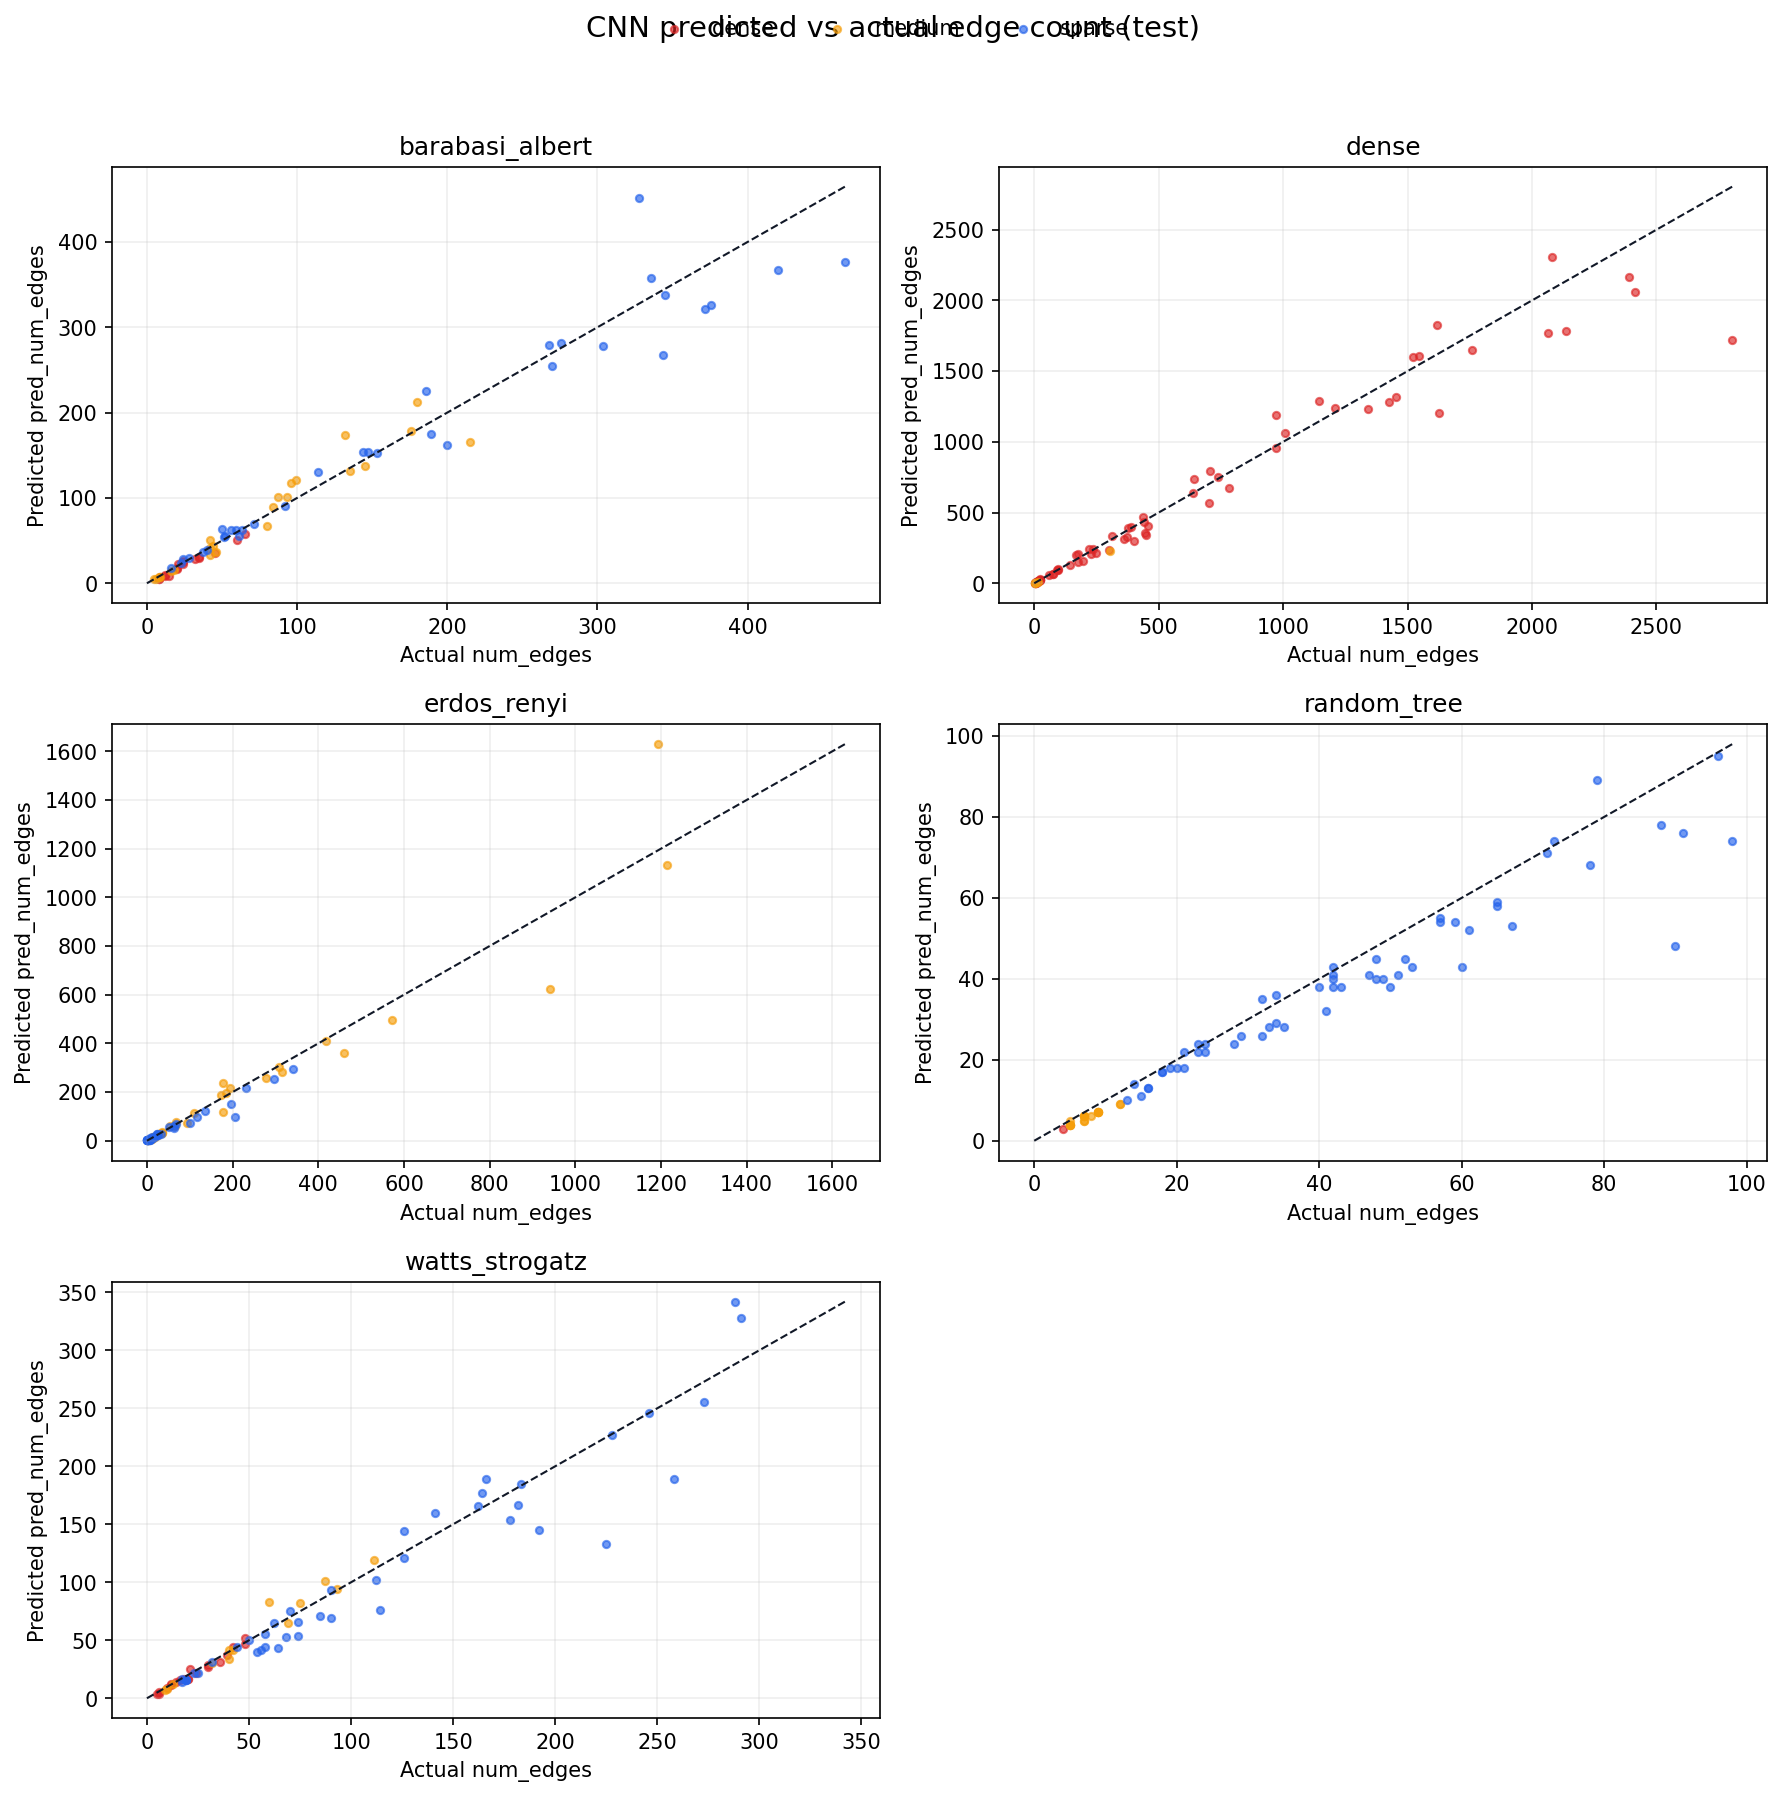
\includegraphics[width=\textwidth, height=0.75\textheight, keepaspectratio]{../figures/cnn_pred_num_edges_scatter_test.png}
        \caption{Edge count predictions (test split).}
        \label{fig:edges_scatter_test}
    \end{subfigure}
    \caption{Scatter plots of predictions vs. ground truth on synthetic test data.}
\end{figure}
\FloatBarrier

\begin{figure}[htbp]
    \centering
    \begin{subfigure}[b]{0.45\textwidth}
        \centering
        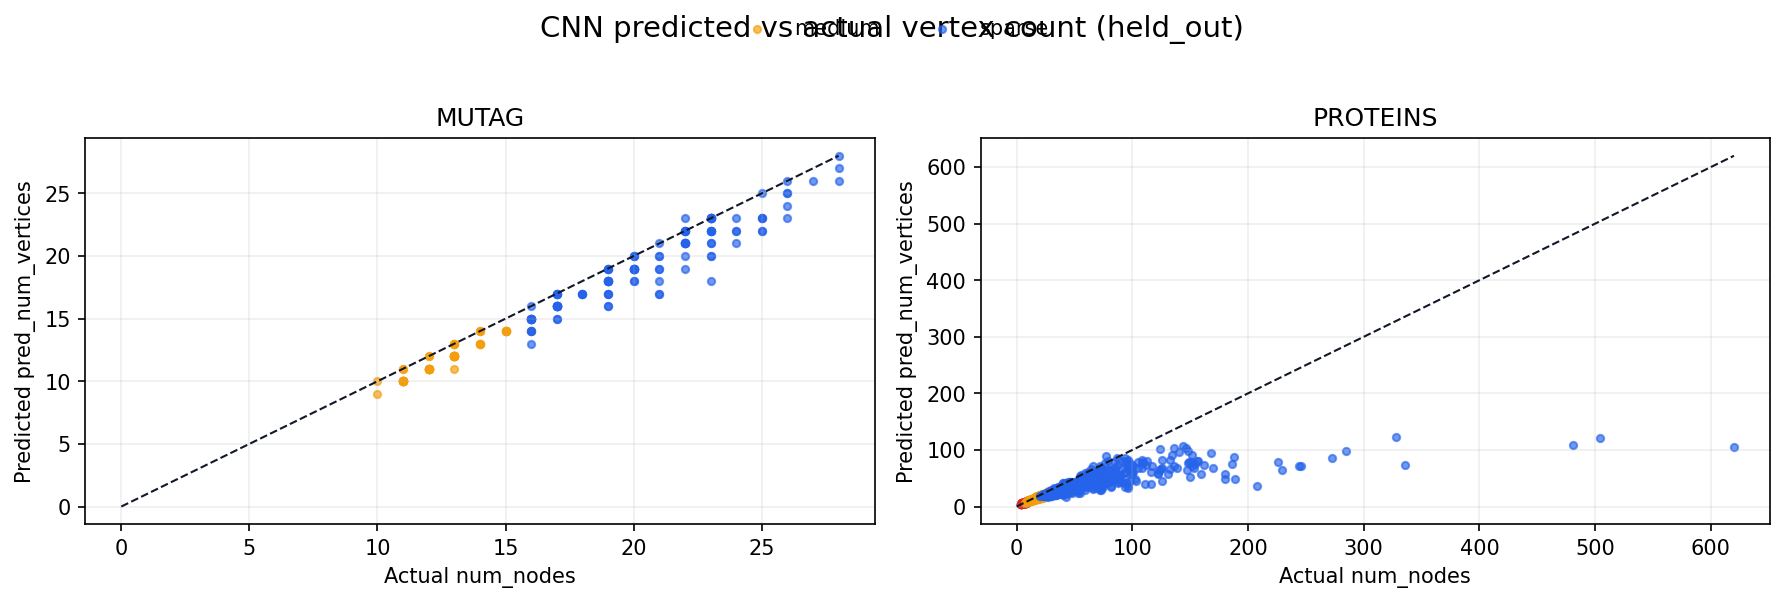
\includegraphics[width=\textwidth, height=0.75\textheight, keepaspectratio]{../figures/cnn_pred_num_vertices_scatter_held_out.png}
        \caption{Vertex count predictions (held-out split).}
        \label{fig:vertices_scatter_held_out}
    \end{subfigure}
    \hfill
    \begin{subfigure}[b]{0.45\textwidth}
        \centering
        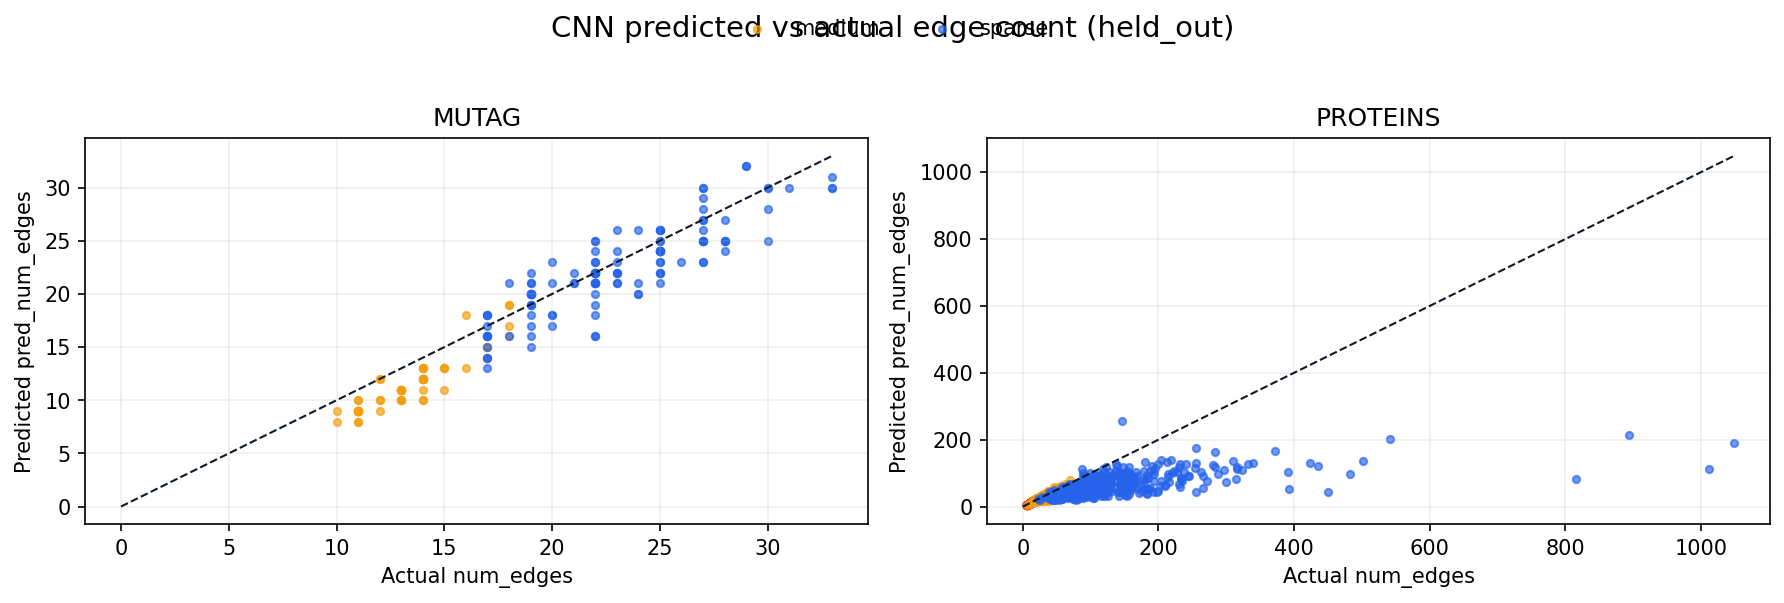
\includegraphics[width=\textwidth, height=0.75\textheight, keepaspectratio]{../figures/cnn_pred_num_edges_scatter_held_out.png}
        \caption{Edge count predictions (held-out split).}
        \label{fig:edges_scatter_held_out}
    \end{subfigure}
    \caption{Scatter plots of predictions vs. ground truth on real held-out data.}
\end{figure}
\FloatBarrier

\begin{table}[htbp]
\centering
\caption{Detailed MAE by Generator Type on the Test Split}
\label{tab:generator_breakdown}
\begin{tabular}{lccccc}
\toprule
Generator & CNN Vertices & GCN Vertices & CNN Edges & GCN Edges & Graph-stat Edges \\
\midrule
barabasi\_albert & 2.83 & 18.68 & 13.80 & 81.53 & 184.23 \\
dense & 1.75 & 21.65 & 75.63 & 497.71 & 76.67 \\
erdos\_renyi & 2.47 & 15.49 & 22.48 & 96.92 & 51.83 \\
random\_tree & 5.69 & 17.71 & 4.77 & 17.60 & 87.81 \\
watts\_strogatz & 3.27 & 21.71 & 10.27 & 51.15 & 202.09 \\
\bottomrule
\end{tabular}
\end{table}

\begin{table}[htbp]
\centering
\caption{Detailed MAE by Dataset on the Held-out Split}
\label{tab:dataset_breakdown}
\begin{tabular}{lccccc}
\toprule
Dataset & CNN Vertices & GCN Vertices & CNN Edges & GCN Edges & Graph-stat Edges \\
\midrule
MUTAG & 1.07 & 5.45 & 1.85 & 17.03 & 24.60 \\
PROTEINS & 12.23 & 23.80 & 32.45 & 63.57 & 420.93 \\
\bottomrule
\end{tabular}
\end{table}

\begin{table}[htbp]
\centering
\caption{Detailed MAE by Density Bucket on the Held-out Split}
\label{tab:density_breakdown}
\begin{tabular}{lccccc}
\toprule
Density Bucket & CNN Vertices & GCN Vertices & CNN Edges & GCN Edges & Graph-stat Edges \\
\midrule
dense & 0.43 & 13.94 & 1.13 & 72.10 & 6.51 \\
medium & 2.03 & 7.57 & 5.91 & 44.96 & 12.63 \\
sparse & 18.75 & 32.13 & 49.11 & 61.90 & 683.54 \\
\bottomrule
\end{tabular}
\end{table}

Two patterns stand out across these breakdowns and are followed up in detail in Section~\ref{ch:interpretation}: first, the CNN's vertex error is lowest specifically on \texttt{dense} graphs and highest on \texttt{sparse} ones (Table~\ref{tab:density_breakdown})---the opposite of what one might naively expect if clutter were the main difficulty, and a pattern that turns out to be connected to the node-size rendering convention rather than to genuine ease of counting. Second, the graph-statistic heuristic's edge error explodes specifically on \texttt{sparse} graphs (683.54), because a single fixed per-generator density estimate is a poor fit for the tail of unusually sparse instances within a family---exactly the failure mode a non-learned heuristic baseline is expected to exhibit.

% ----------------------------------------------------------------------
% SECTION 8: MODEL INTERPRETATION & FAILURE ANALYSIS
% ----------------------------------------------------------------------
\section{Model Interpretation \& Failure Analysis}
\label{ch:interpretation}
Section~\ref{sec:results} answered the Competitiveness question from the Introduction: the CNN beats the GCN baseline on every metric. This chapter exists to answer the harder Mechanism question---\emph{why}---since a strong accuracy number alone cannot distinguish a model that has learned genuine structural reasoning from one that has found an easier shortcut that merely correlates with the correct answer on this particular rendering pipeline. Each section below is a separate, targeted probe designed to rule in or rule out a specific candidate explanation, moving from a qualitative look at what the network attends to (Grad-CAM), to a direct causal intervention on the strongest suspected confound (the node-size probe), to statistical significance testing of that intervention, to an alternative low-level explanation (pixel counting), to a systematic characterization of where errors concentrate, and finally to an end-to-end validation against the deployed application itself.

\subsection{Grad-CAM Spatial Attributions}
Grad-CAM~[\ref{ref:gradcam}] heatmaps are computed at the final convolutional layer (\texttt{features[3]}, resolution $14 \times 14$) as a first, qualitative pass at the Mechanism question: before running any targeted intervention, it is worth simply visualizing where in the image the network's gradients concentrate, since a model attending to background canvas or to arbitrary corners would already be a red flag before any quantitative probe is needed.
\begin{itemize}
    \item \textbf{Attribution Focus:} Activation is concentrated on the spatial locations of node clusters rather than the background canvas, as shown in the generator grid (Figure~\ref{fig:gradcam_generators}). This is a reassuring baseline sanity check---the model is at least looking at the graph rather than at rendering artifacts elsewhere in the frame.
    \item \textbf{Edge vs. Vertex Attributions:} The vertex-target maps are tightly localized around individual node boundaries, whereas the edge-target maps are diffuse, covering the structural gaps between nodes. This distinction is intuitive: counting vertices is a localized, per-blob task, while counting edges requires attending to the connective tissue between blobs, so the two output heads would be expected to draw on different spatial evidence even though they share the same convolutional trunk.
    \item \textbf{Failure Activation:} Worst-error cases exhibit activation concentrated on a single cluster rather than spreading across the entire graph boundary, revealing a spatial attention bottleneck (visualized in Figure~\ref{fig:gradcam_failures})---consistent with the size-generalization failures quantified later in Section~\ref{ch:interpretation}.6, where large graphs that do not fit the network's learned notion of ``how big a graph looks'' produce disproportionately large errors.
\end{itemize}

\begin{figure}[htbp]
    \centering
    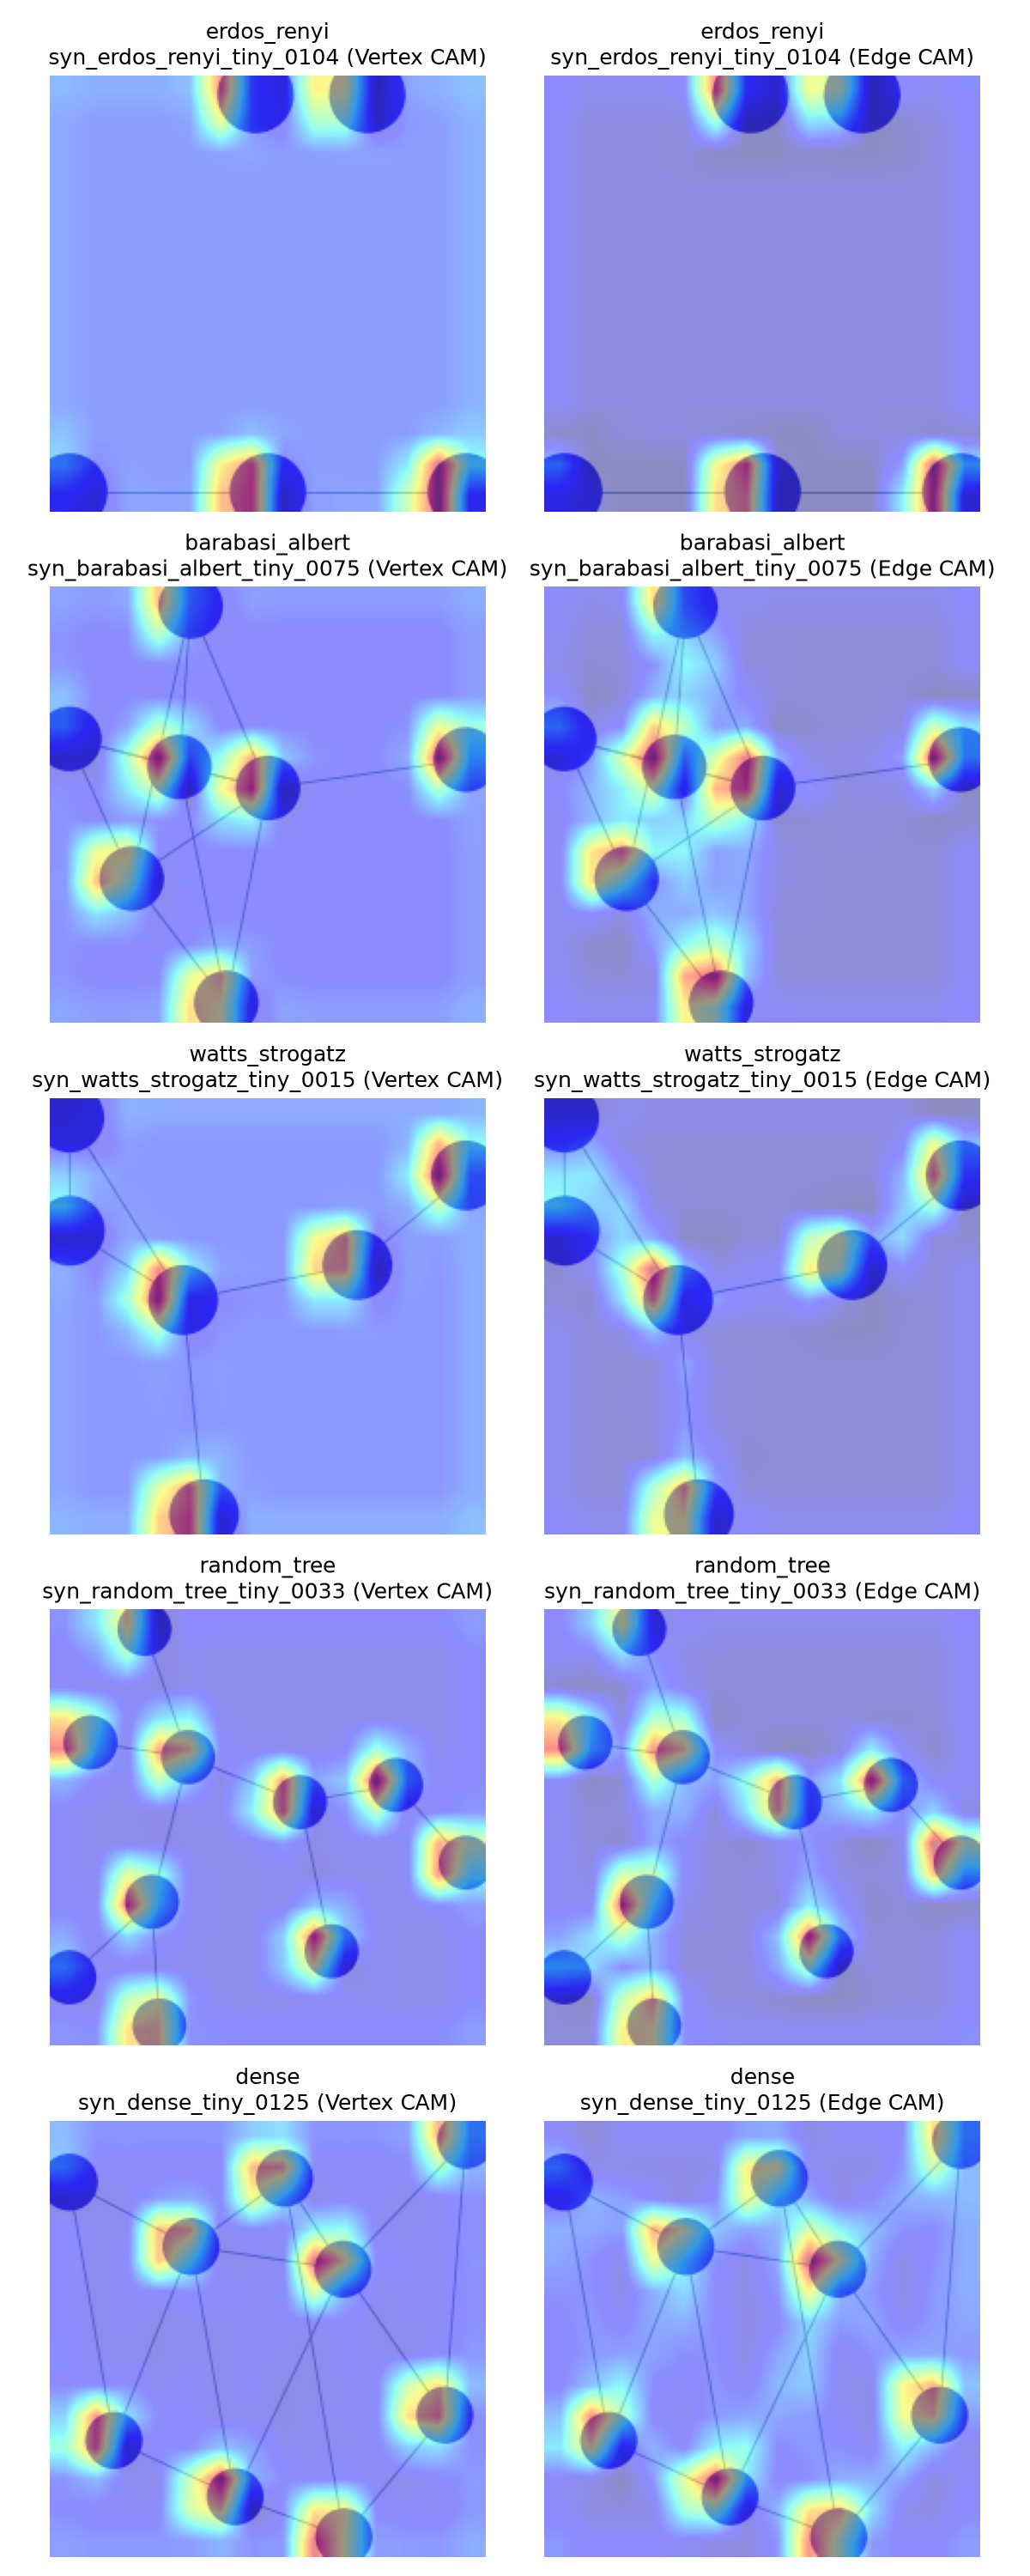
\includegraphics[width=0.8\textwidth, height=0.75\textheight, keepaspectratio]{../figures/gradcam_grid_by_generator.png}
    \caption{Grad-CAM activations mapped across representatives of each generator family.}
    \label{fig:gradcam_generators}
\end{figure}
\FloatBarrier

\begin{figure}[htbp]
    \centering
    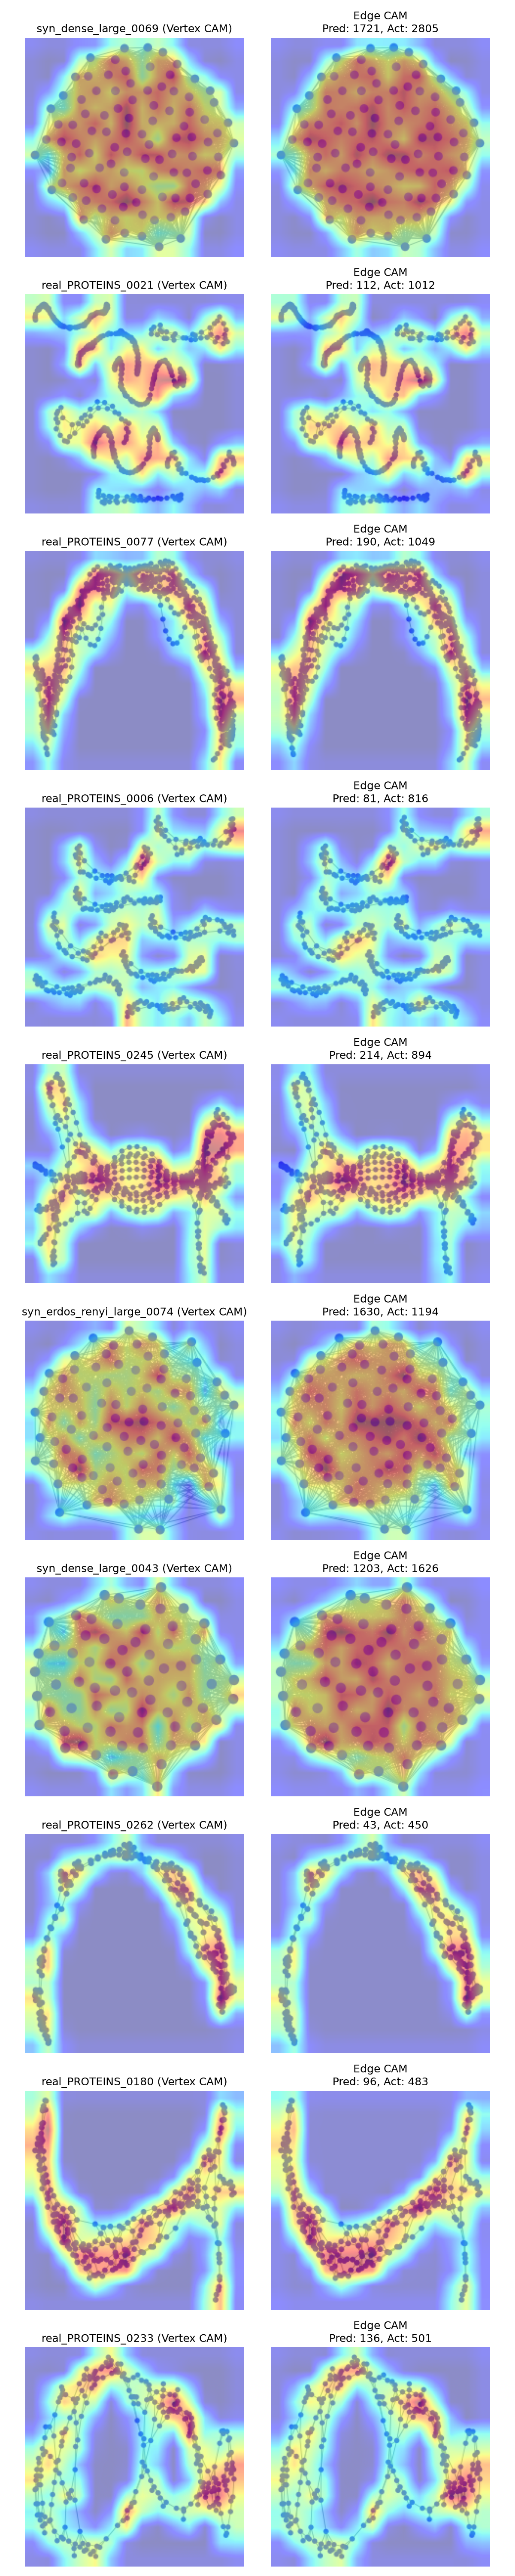
\includegraphics[width=0.8\textwidth, height=0.75\textheight, keepaspectratio]{../figures/gradcam_grid_failure_cases.png}
    \caption{Grad-CAM activations on high-error failure cases.}
    \label{fig:gradcam_failures}
\end{figure}
\FloatBarrier

\subsection{Shortcut-Learning Probe (Node-Size)}
The rendering formula in Section~\ref{sec:rendering} (Equation~\ref{eq:node_radius}) was flagged at design time as a potential shortcut, since node radius is a deterministic function of vertex count and therefore a trivially exploitable proxy. This section tests that hypothesis directly rather than leaving it as a hypothesis. To test the node-size shortcut directly, we re-rendered a probe set of 40 graphs (10 per tier) with a constant node size, holding layout positions and edge widths fixed---if the model's accuracy depends on the true visual size cue rather than on genuine topological reasoning, removing it while holding everything else constant should degrade accuracy measurably. Examples of these probe variants are visualized in Figure~\ref{fig:probe_examples}, and the tier-wise MAE comparisons are plotted in Figure~\ref{fig:probe_mae}. Table~\ref{tab:probe_summary} displays the numeric results. The overall vertex MAE triples from 3.425 to 10.475 when the size cue is removed, confirming that the model heavily exploits node-size inverse scaling.

\begin{figure}[htbp]
    \centering
    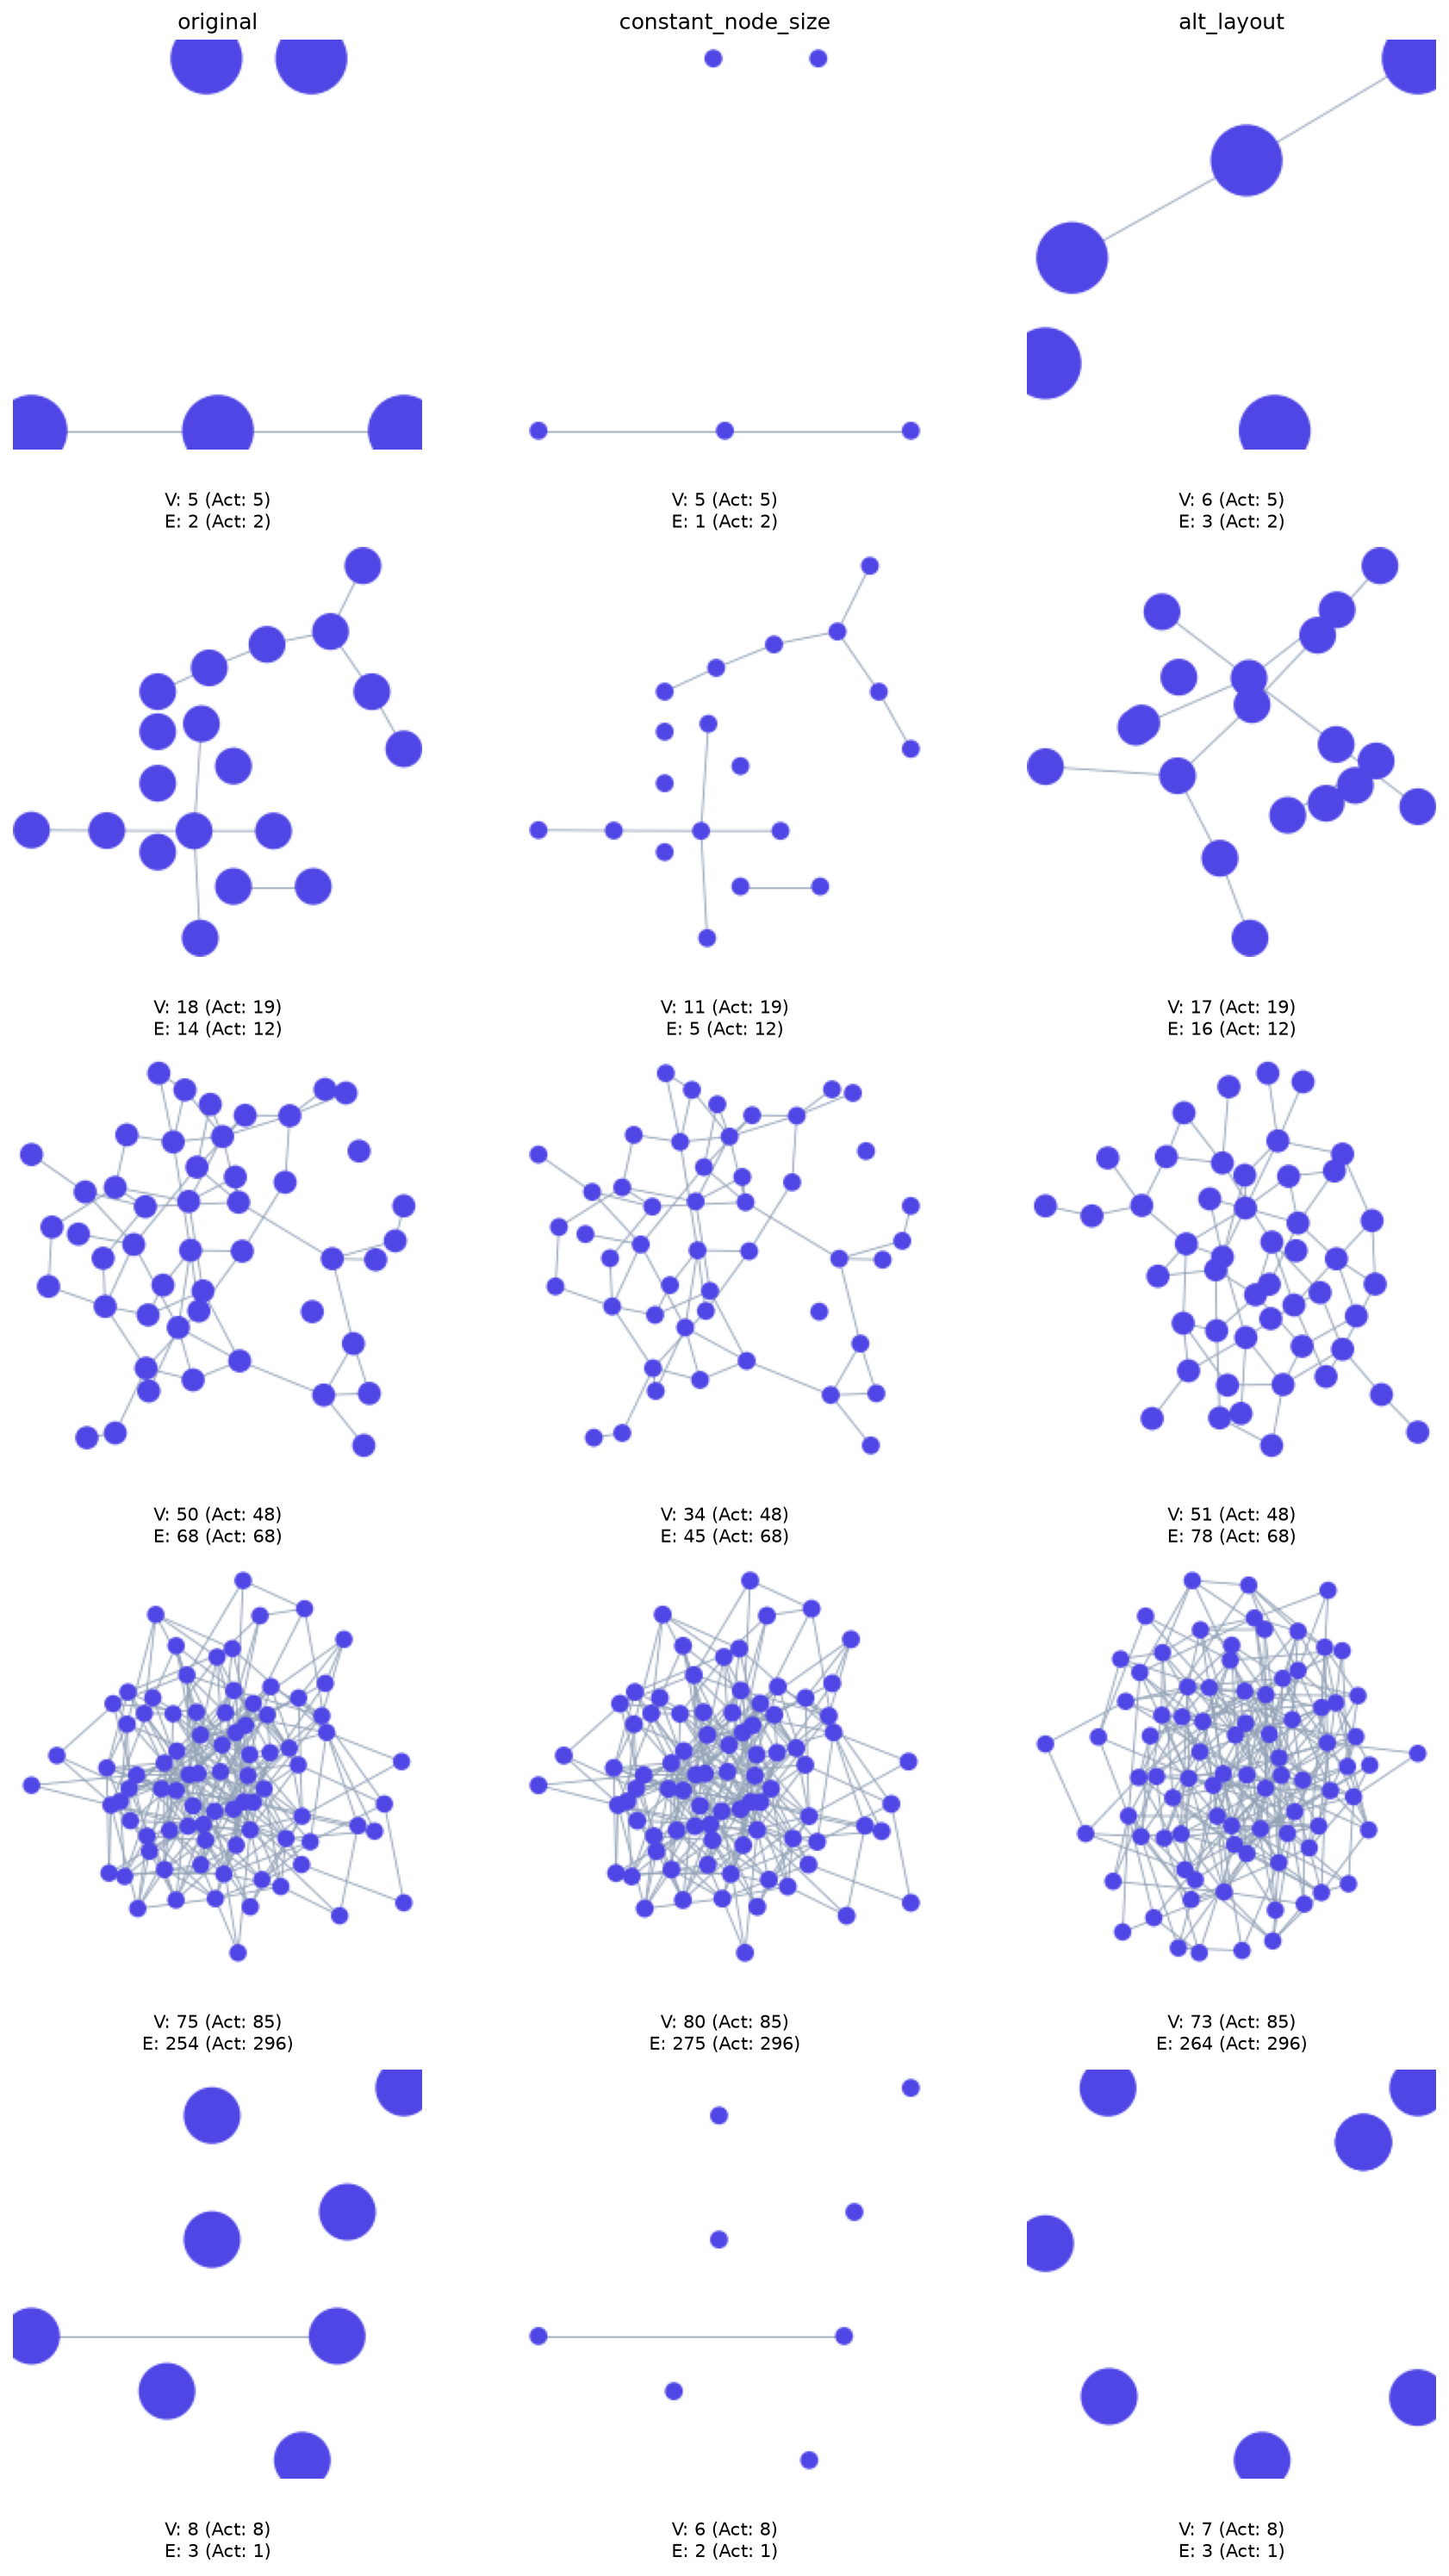
\includegraphics[width=0.8\textwidth, height=0.75\textheight, keepaspectratio]{../figures/probe_variant_examples_grid.png}
    \caption{Side-by-side comparison of original, constant node-size, and alternative layouts.}
    \label{fig:probe_examples}
\end{figure}
\FloatBarrier

\begin{figure}[htbp]
    \centering
    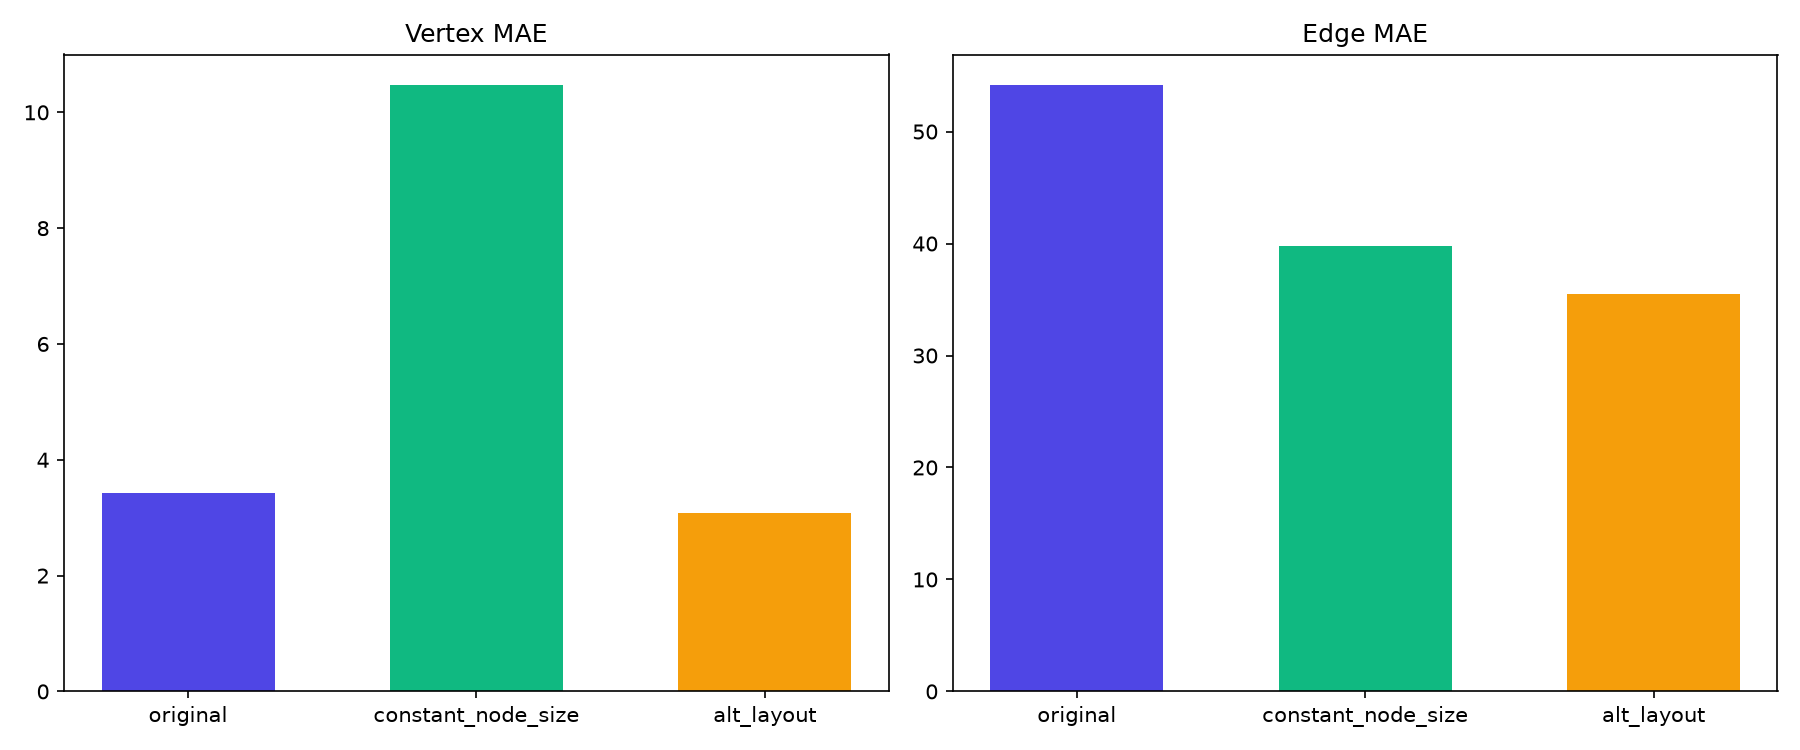
\includegraphics[width=0.6\textwidth, height=0.75\textheight, keepaspectratio]{../figures/probe_variant_mae_comparison.png}
    \caption{Error comparison (MAE) across the different probe variants.}
    \label{fig:probe_mae}
\end{figure}
\FloatBarrier

\begin{table}[htbp]
\centering
\caption{Probe Summary MAE by Variant and Size Tier}
\label{tab:probe_summary}
\footnotesize
\begin{tabular}{lcccccc}
\toprule
Tier & Orig. Vert. & Fixed Vert. & Alt Vert. & Orig. Edges & Fixed Edges & Alt Edges \\
\midrule
tiny & 0.3 & 1.4 & 0.4 & 1.6 & 3.5 & 1.6 \\
small & 1.0 & 8.5 & 1.0 & 3.3 & 21.2 & 4.9 \\
medium & 3.5 & 15.3 & 3.8 & 16.3 & 51.7 & 13.2 \\
large & 8.9 & 16.7 & 7.1 & 195.5 & 82.8 & 122.4 \\
\midrule
Overall & 3.425 & 10.475 & 3.075 & 54.175 & 39.8 & 35.525 \\
\bottomrule
\end{tabular}
\end{table}

\subsection{Layout-Sensitivity Probe}
The node-size probe isolates one candidate shortcut, but layout geometry itself---the specific $(x,y)$ coordinates \texttt{sfdp} happens to produce---is a second plausible confound, since the CNN could in principle be keying off Graphviz-specific spatial patterns rather than the topology those patterns represent. We re-rendered the 40 probe graphs using a Kamada-Kawai layout instead of Graphviz \texttt{sfdp}. The results (Table~\ref{tab:probe_summary}) show that the model's accuracy remains stable, indicating that the CNN is layout-insensitive within this family and did not overfit to Graphviz-specific coordinates.

\subsection{Wilcoxon Signed-Rank Tests}
The mean-MAE comparisons above are suggestive but vulnerable to distortion by a handful of outlier graphs, as the edge-count results in this very section demonstrate. A paired Wilcoxon signed-rank test~[\ref{ref:wilcoxon}] is used instead because it is a non-parametric test on the direction and rank of per-graph differences rather than their raw magnitude, making it far more robust to exactly this kind of outlier distortion, and because the probe design (each of the 40 graphs rendered under two conditions) naturally produces paired observations. The test ($n=40$) confirms that removing the node-size cue significantly degrades vertex prediction ($p = 3.5799 \times 10^{-6}$, 33/40 graphs worse) and edge prediction ($p = 2.9778 \times 10^{-4}$, 35/40 graphs worse). In contrast, the layout intervention shows a clean null result ($p = 0.4991$ for vertices, $p = 0.8978$ for edges), validating that layout change does not affect accuracy significantly (see Table~\ref{tab:wilcoxon_tests}). Together, these two tests separate the two candidate confounds cleanly: node size is a real, statistically significant driver of accuracy, while layout geometry is not.

\begin{table}[htbp]
\centering
\caption{Wilcoxon Signed-Rank Test Results for Node-Size and Layout Probes ($n=40$)}
\label{tab:wilcoxon_tests}
\small
\resizebox{\textwidth}{!}{%
\begin{tabular}{lllccccc}
\toprule
Probe Intervention & Target & Original Mean (Median) & Intervention Mean (Median) & Worse/Better/Tie & Wilcoxon Stat & $p$-value & Signif. (0.05) \\
\midrule
Fixed Node Size & Vertices & 3.425 (1.0) & 10.475 (11.0) & 33 / 4 / 3 & 44.5 & $3.58 \times 10^{-6}$ & Yes \\
& Edges & 54.175 (3.5) & 39.8 (20.0) & 35 / 5 / 0 & 141.0 & $2.98 \times 10^{-4}$ & Yes\textsuperscript{*} \\
\midrule
Alt. Layout (KK) & Vertices & 3.425 (1.0) & 3.075 (1.0) & 17 / 16 / 7 & 243.5 & 0.4991 & No \\
& Edges & 54.175 (3.5) & 35.525 (4.5) & 18 / 16 / 6 & 290.0 & 0.8978 & No \\
\bottomrule
\end{tabular}%
}
\begin{flushleft}
\small \textsuperscript{*} Although the mean error decreases due to outliers, the Wilcoxon test ranks confirm a significant worsening pattern for the 35/40 majority.
\end{flushleft}
\end{table}

\subsection{Ink-Coverage Correlational Analysis}
The node-size probe rules in one confound, but a simpler explanation is still worth ruling out before crediting the model with any structural understanding at all: perhaps the CNN is not reasoning about discrete nodes and edges in any meaningful sense, but is simply performing regression against the total amount of ink on the page. We correlated predicted/true targets against low-level pixel statistics: \texttt{ink\_fraction} (non-background pixels) and \texttt{mean\_component\_area}. Visual scatter diagrams of these relationships are provided in Figure~\ref{fig:ink_vs_nodes} and Figure~\ref{fig:component_size_vs_nodes}. The resulting correlation statistics are shown in Table~\ref{tab:ink_coverage_correlations}.

\begin{figure}[htbp]
    \centering
    \begin{subfigure}[b]{0.45\textwidth}
        \centering
        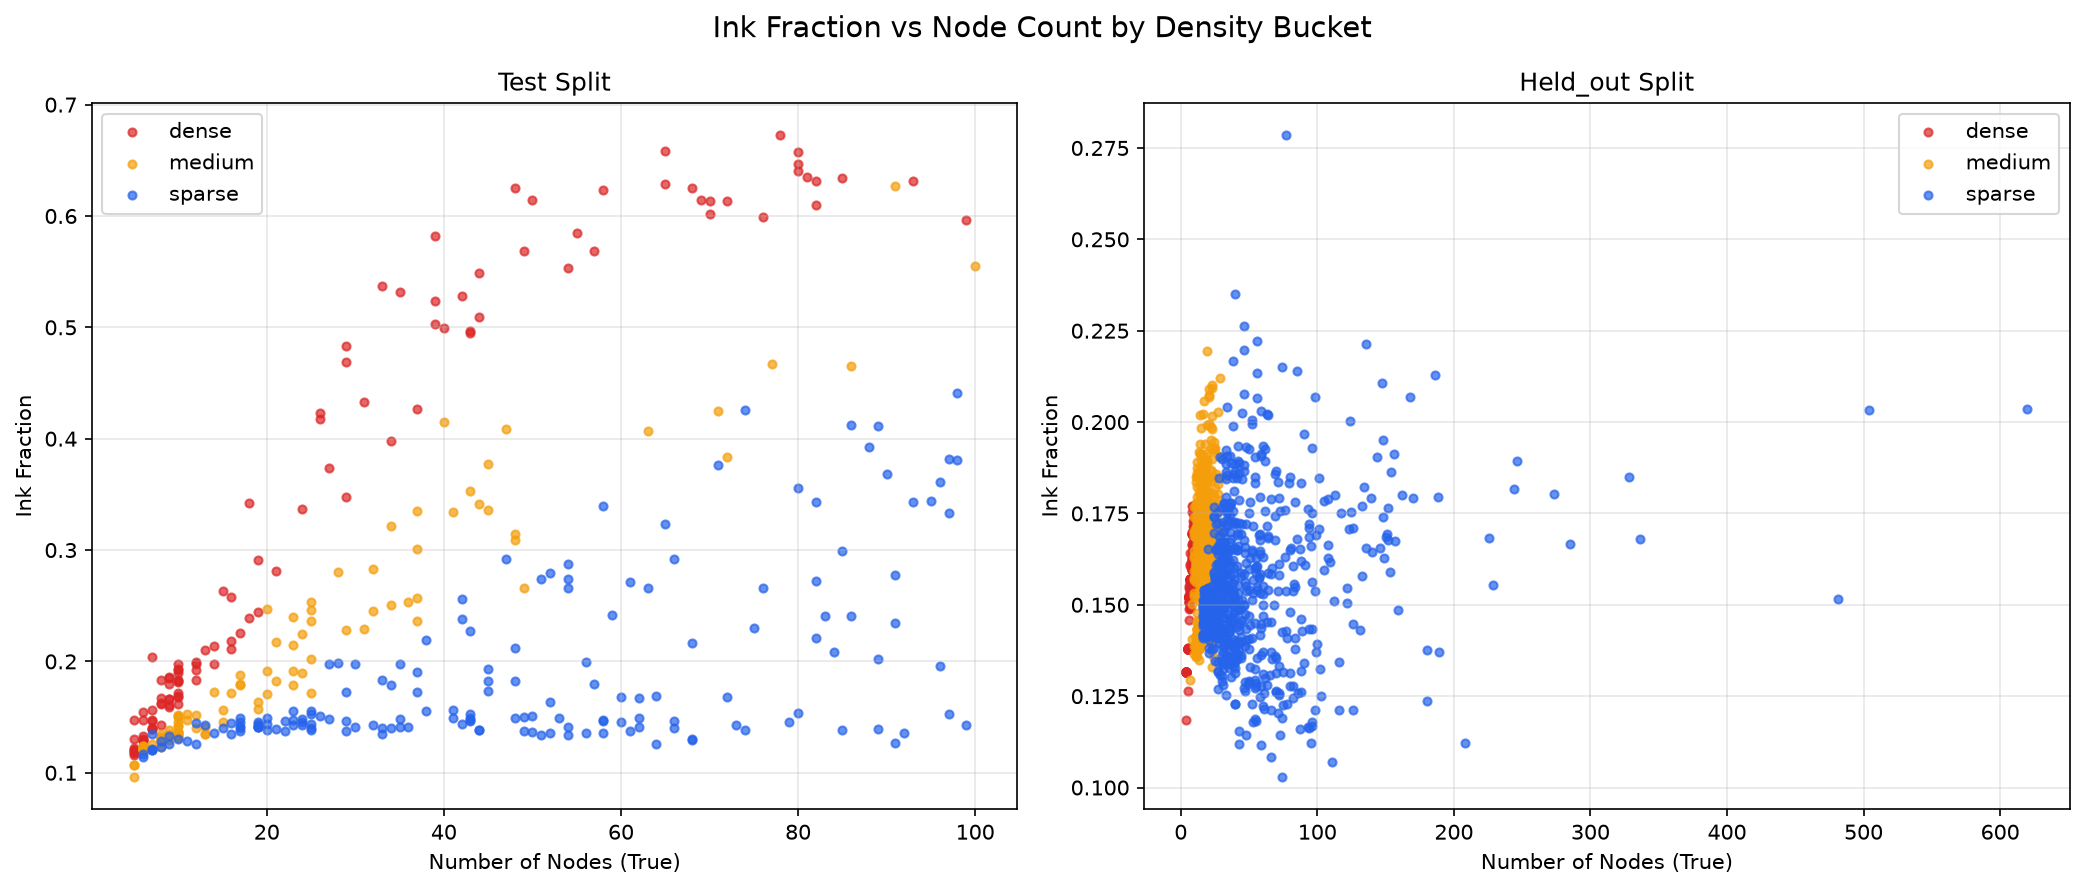
\includegraphics[width=\textwidth, height=0.75\textheight, keepaspectratio]{../figures/ink_coverage_vs_node_count.png}
        \caption{Ink fraction vs. node count.}
        \label{fig:ink_vs_nodes}
    \end{subfigure}
    \hfill
    \begin{subfigure}[b]{0.45\textwidth}
        \centering
        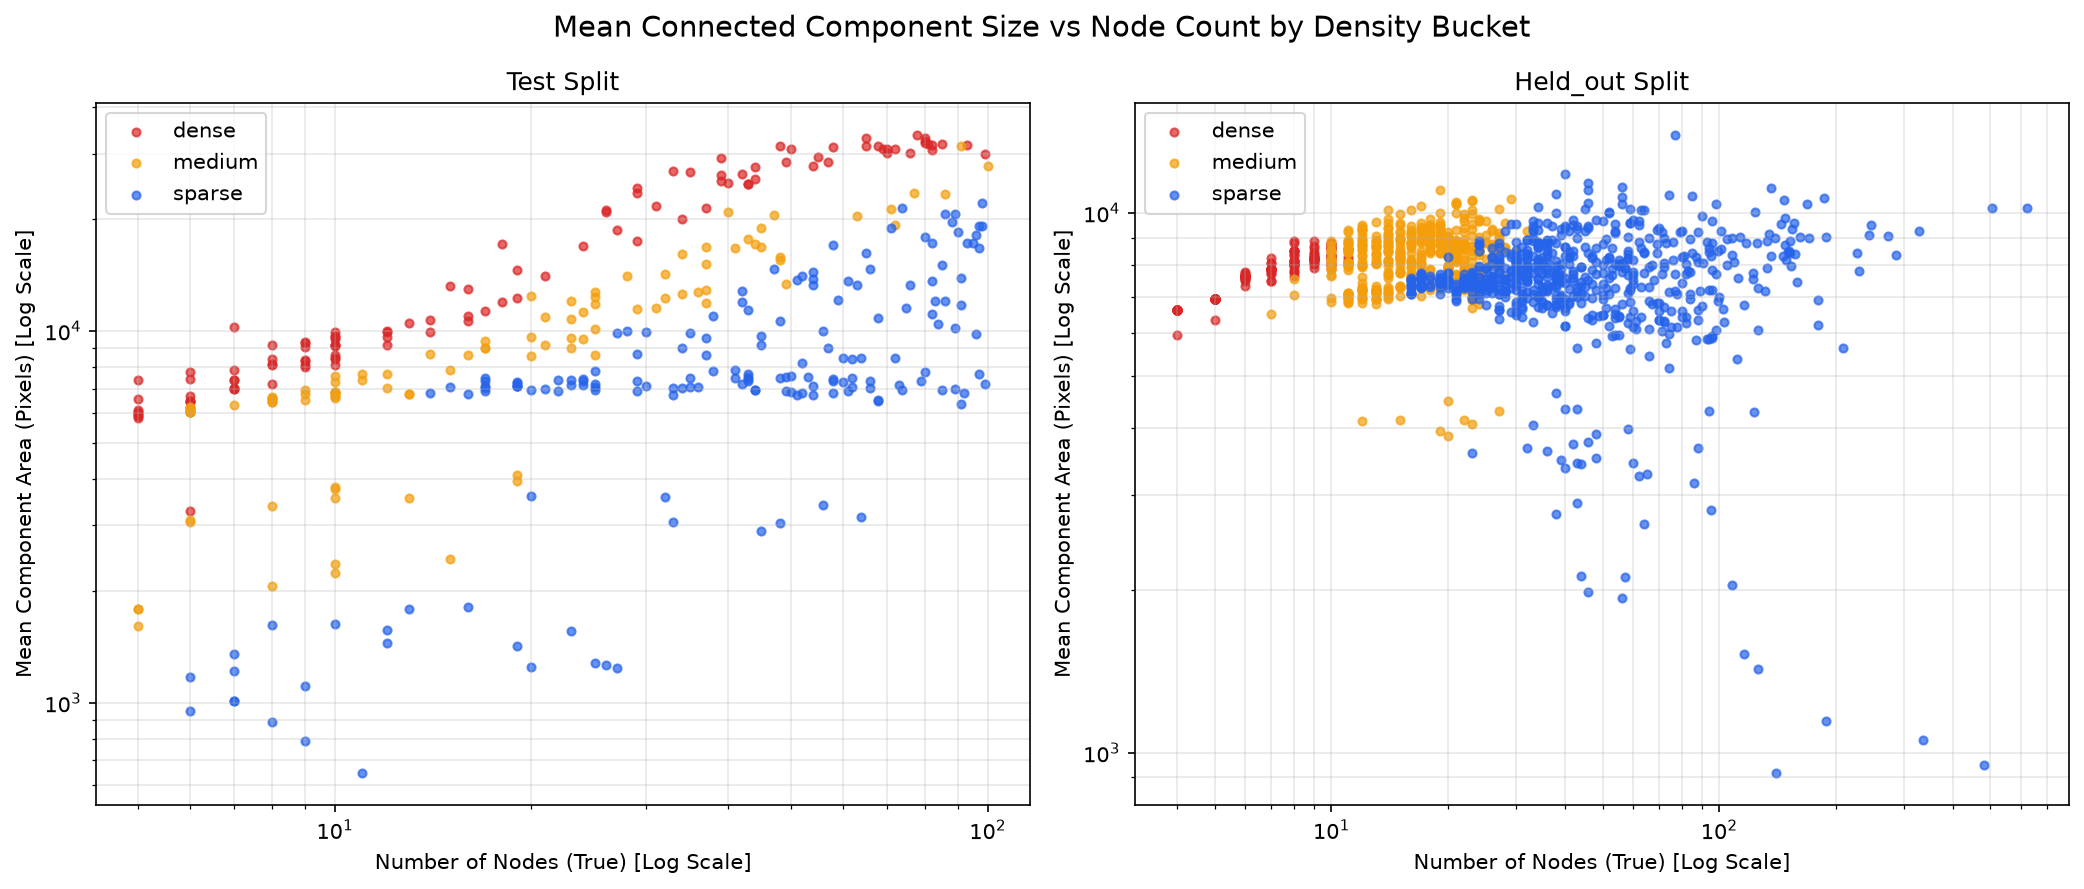
\includegraphics[width=\textwidth, height=0.75\textheight, keepaspectratio]{../figures/component_size_vs_node_count.png}
        \caption{Component area vs. node count.}
        \label{fig:component_size_vs_nodes}
    \end{subfigure}
    \caption{Correlations between visual pixel properties and actual node counts.}
\end{figure}
\FloatBarrier

\begin{table}[htbp]
\centering
\caption{Pearson Correlations ($r$) for Low-Level Pixel Statistics vs. True and Predicted Graph Properties}
\label{tab:ink_coverage_correlations}
\resizebox{\textwidth}{!}{%
\begin{tabular}{llcccc}
\toprule
Metric X & Metric Y & Test Split $r$ & Test Split $p$ & Held-out Split $r$ & Held-out Split $p$ \\
\midrule
ink\_fraction & num\_nodes & 0.5378 & $1.72 \times 10^{-29}$ & 0.0700 & 0.0115 \\
ink\_fraction & num\_edges & 0.8235 & $7.48 \times 10^{-94}$ & 0.0930 & $7.84 \times 10^{-4}$ \\
ink\_fraction & pred\_num\_vertices & 0.6182 & $6.59 \times 10^{-41}$ & 0.1722 & $4.04 \times 10^{-10}$ \\
ink\_fraction & pred\_num\_edges & 0.8453 & $1.49 \times 10^{-103}$ & 0.4654 & $6.58 \times 10^{-71}$ \\
mean\_component\_area & num\_nodes & 0.5521 & $2.66 \times 10^{-31}$ & -0.0830 & 0.0027 \\
mean\_component\_area & pred\_num\_vertices & 0.6272 & $2.10 \times 10^{-42}$ & 0.0010 & 0.9705 \\
num\_components & num\_nodes & -0.2403 & $2.52 \times 10^{-6}$ & 0.3081 & $5.29 \times 10^{-30}$ \\
\bottomrule
\end{tabular}%
}
\end{table}

On the test split, ink fraction correlates strongly with predicted edge count ($r=0.8453$). A linear baseline fit of \texttt{ink\_fraction} to \texttt{num\_edges} explains 82\% of the variance ($R^2=0.8192$, MAE=83.73).
On the held-out split, however, this correlation collapses completely ($r=0.0930$, $R^2=0.0035$, MAE=47.25), proving that the CNN is not merely counting pixels to generalize to real graphs. An ink-fraction measurement inconsistency exists between the two analytical scripts: one uses \texttt{white\_threshold=250} ($r=0.8235$) and the other uses \texttt{bg\_threshold=200} ($r=0.9051$).

\subsection{Failure Taxonomy Analysis}
The probes above establish \emph{that} shortcuts exist; this section asks \emph{where} the model actually fails in practice, which matters for anyone deciding whether to trust a given prediction. Graphs are categorized into three bins: \texttt{out\_of\_distribution\_size} ($N > 100$), \texttt{high\_density\_clutter} (density $\ge 0.40$), and \texttt{in\_distribution\_normal} (density $< 0.40$). The errors are plotted as functions of size and density in Figure~\ref{fig:error_vs_nodes} and Figure~\ref{fig:error_vs_density}. The categorization summary is given in Table~\ref{tab:failure_taxonomy}.
Size extrapolation is the dominant failure mode, producing catastrophic error rates (mean vertex MAE of 96.64). Conversely, density-driven visual clutter is not a failure mode; \texttt{high\_density\_clutter} graphs produce the lowest errors (mean vertex MAE of 0.43)---this is the same pattern already visible in the density-bucket breakdown in Section~\ref{sec:results}, and is consistent with the node-size shortcut identified above: dense graphs at a given node count render with small, sharply-scaled nodes (via Equation~\ref{eq:node_radius}), giving the model a strong, unambiguous size cue to exploit, whereas sparse and especially oversized graphs fall outside the range of node sizes seen during training. Images that produced the highest overall prediction errors are displayed in Figure~\ref{fig:worst_cases}.

\begin{figure}[htbp]
    \centering
    \begin{subfigure}[b]{0.45\textwidth}
        \centering
        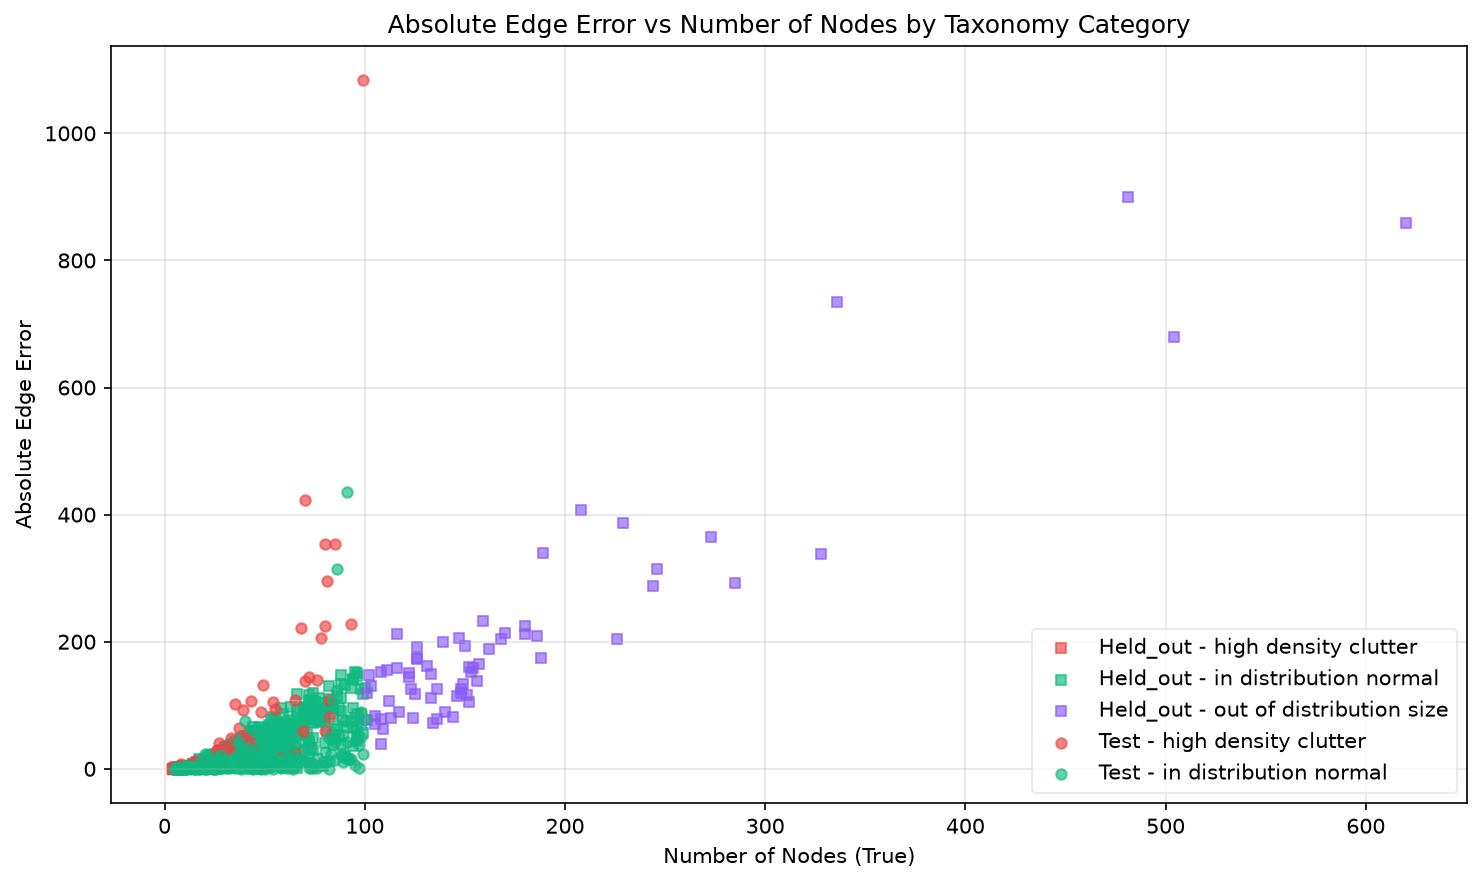
\includegraphics[width=\textwidth, height=0.75\textheight, keepaspectratio]{../figures/error_vs_num_nodes.png}
        \caption{Error vs. node count.}
        \label{fig:error_vs_nodes}
    \end{subfigure}
    \hfill
    \begin{subfigure}[b]{0.45\textwidth}
        \centering
        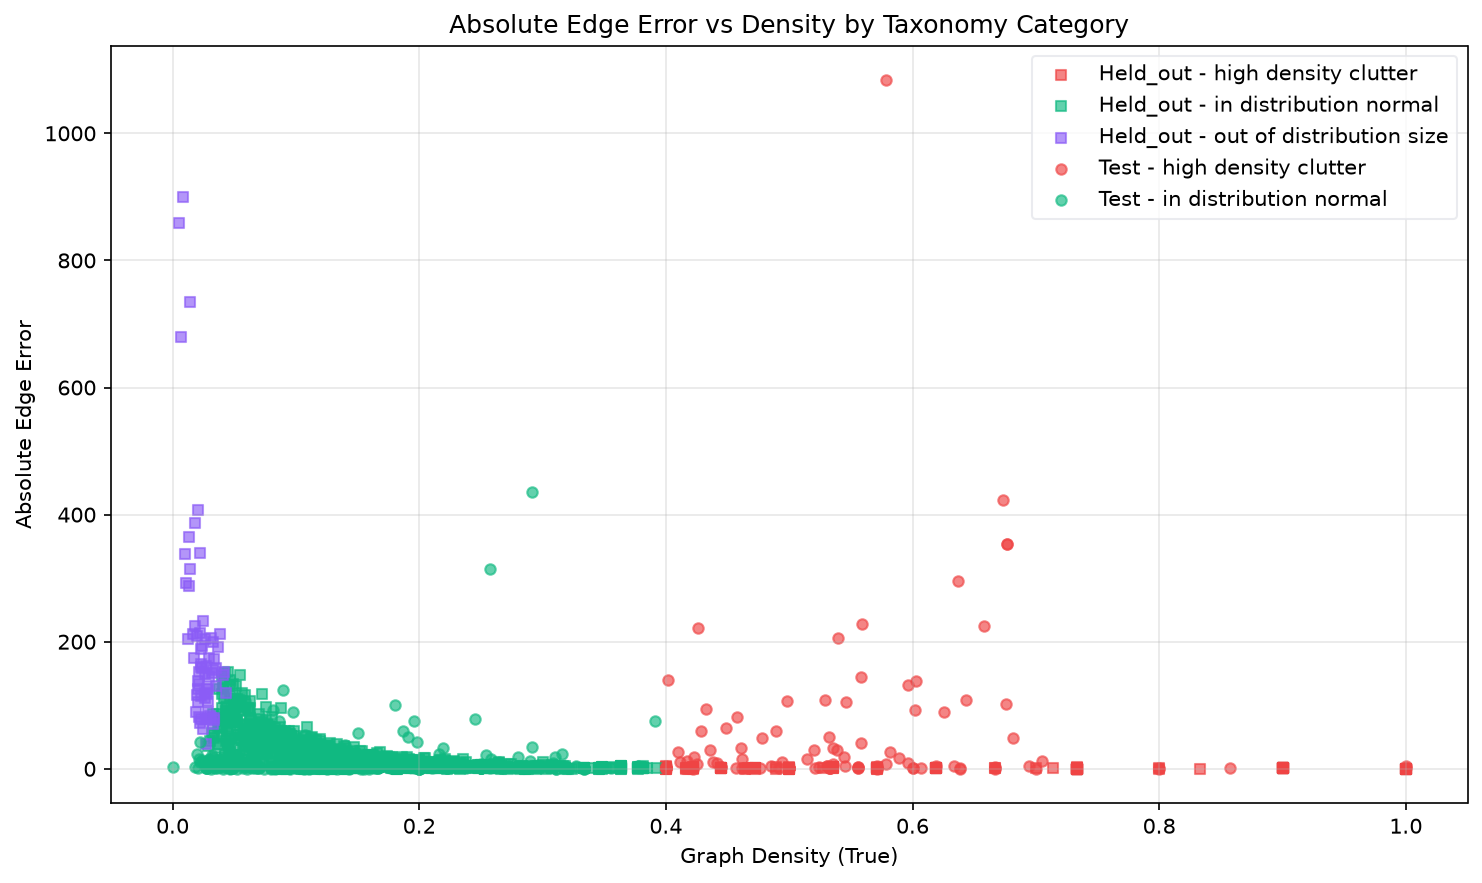
\includegraphics[width=\textwidth, height=0.75\textheight, keepaspectratio]{../figures/error_vs_density.png}
        \caption{Error vs. density.}
        \label{fig:error_vs_density}
    \end{subfigure}
    \caption{Plotting prediction error against physical graph size and structural density.}
\end{figure}
\FloatBarrier

\begin{figure}[htbp]
    \centering
    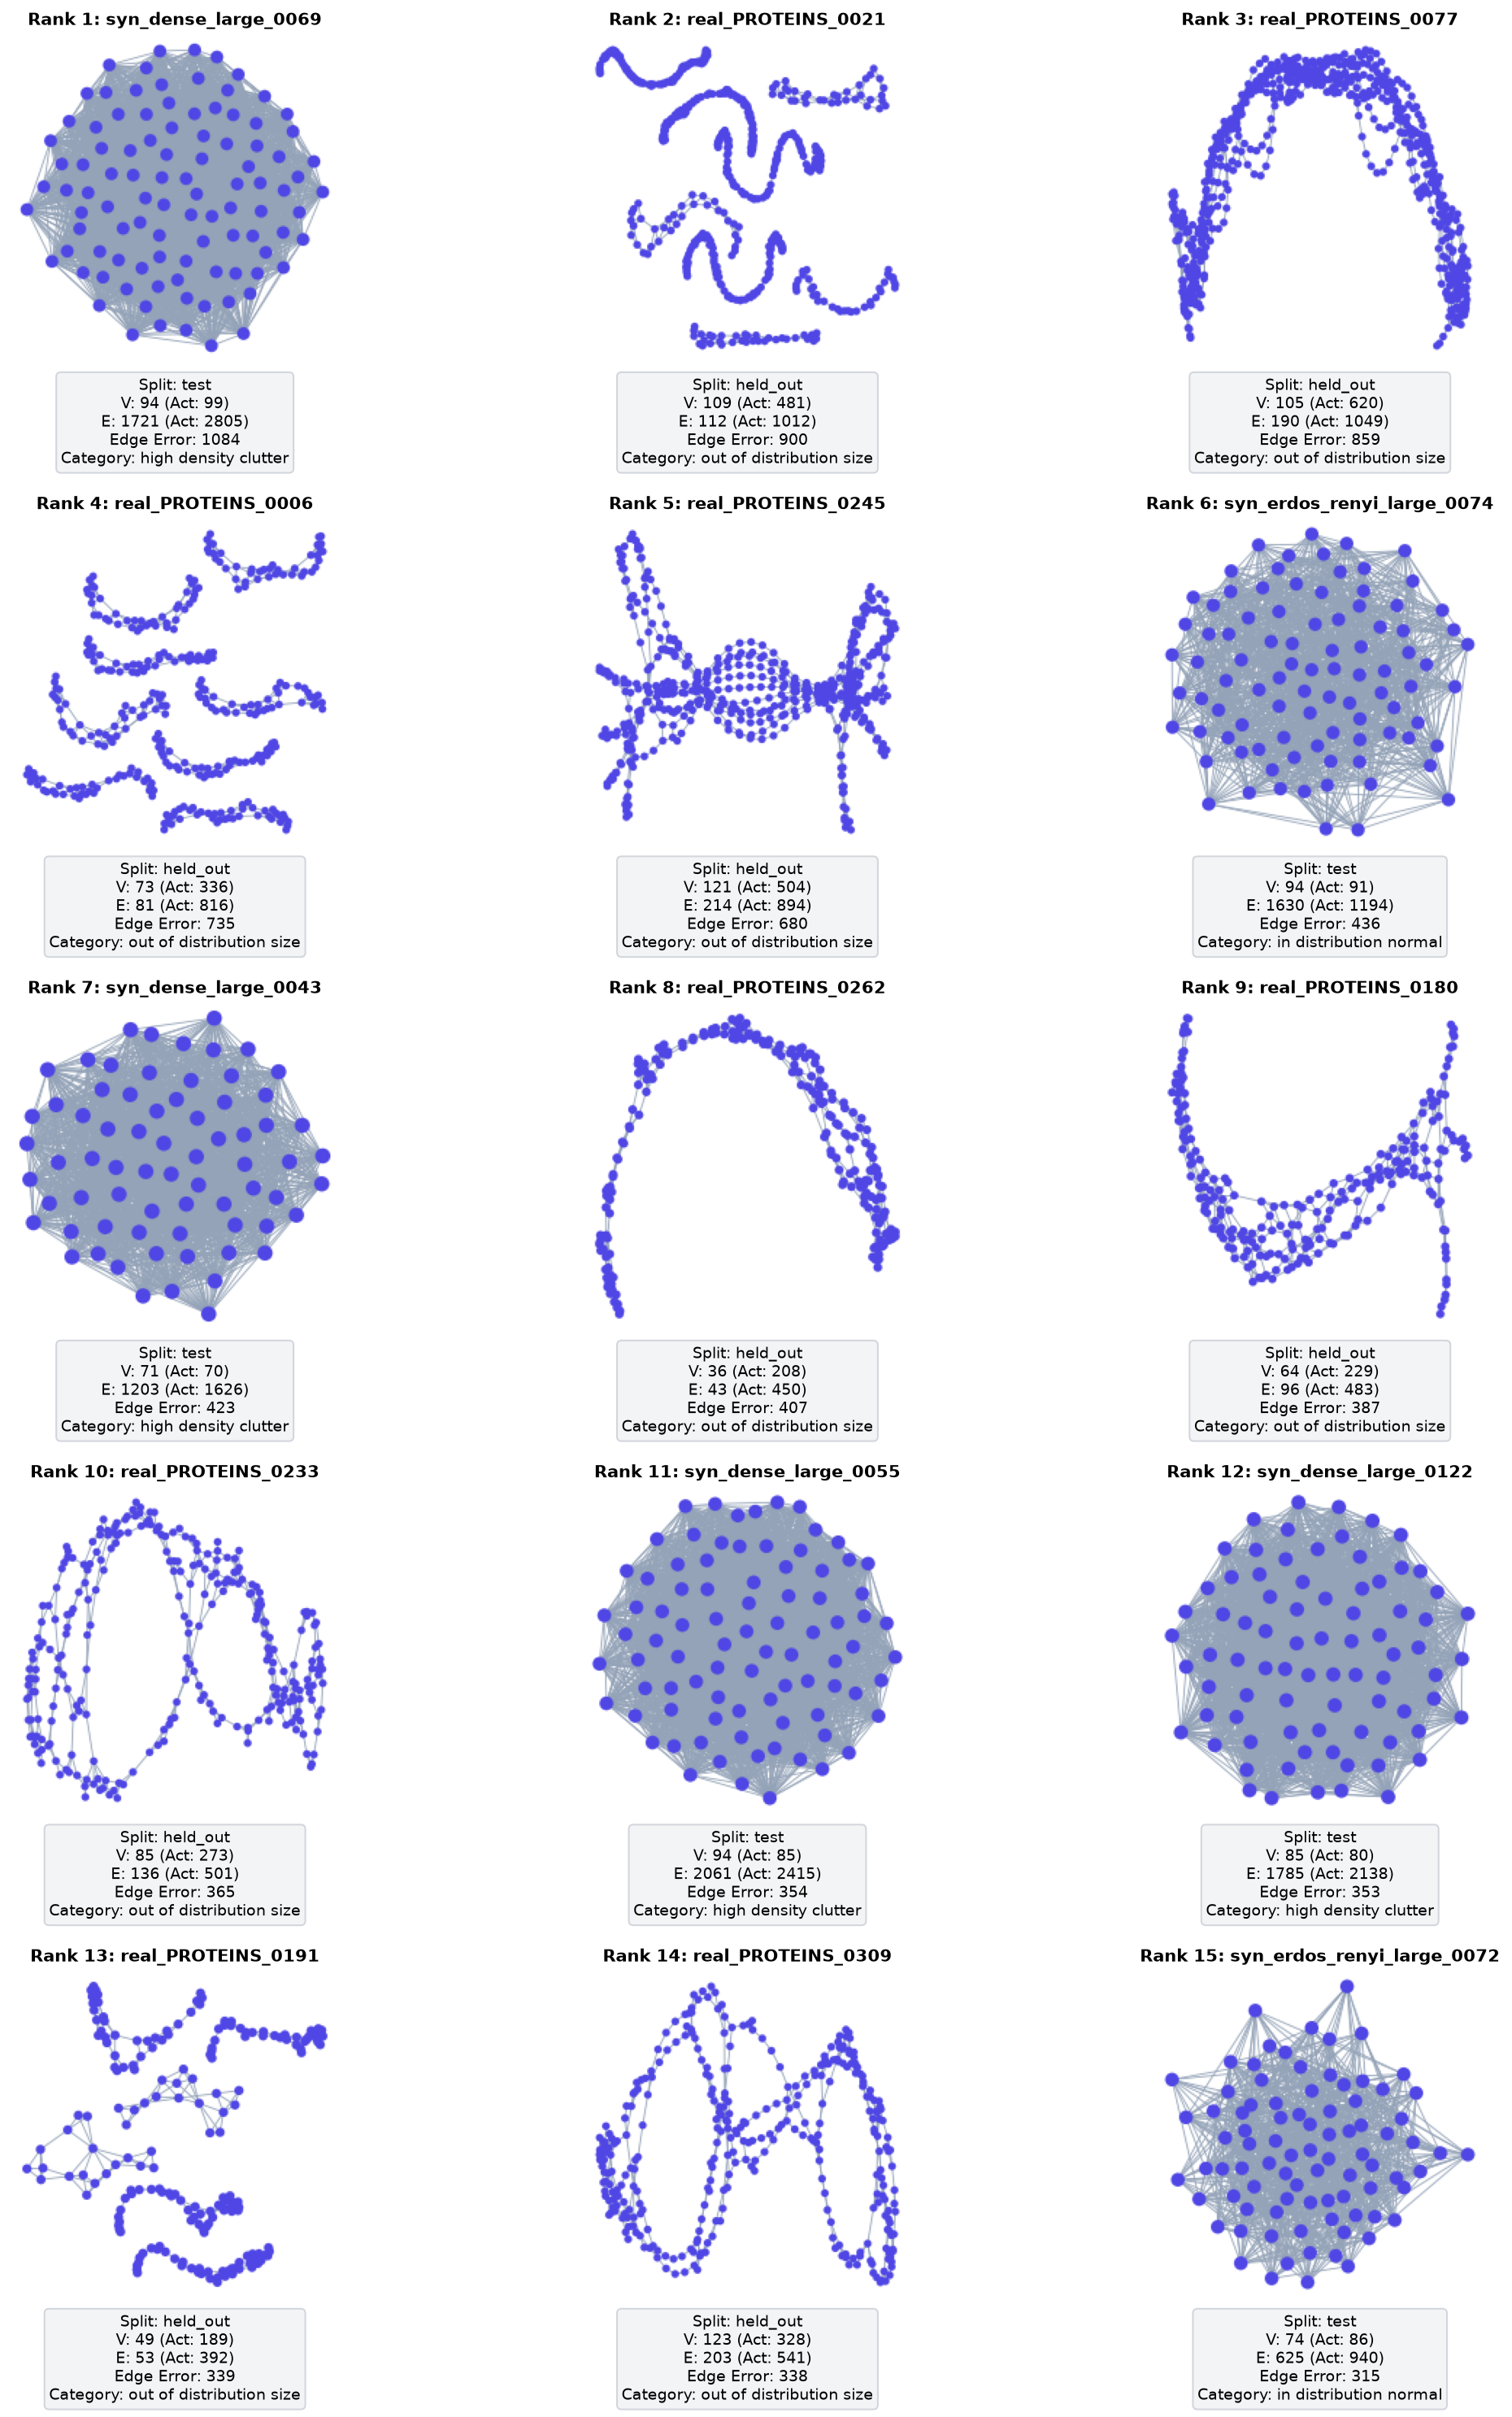
\includegraphics[width=0.8\textwidth, height=0.75\textheight, keepaspectratio]{../figures/worst_case_image_grid.png}
    \caption{Grid of worst-performing outlier images yielding highest regression errors.}
    \label{fig:worst_cases}
\end{figure}
\FloatBarrier

\begin{table}[htbp]
\centering
\caption{Failure Taxonomy Error Analysis (CNN Regressor)}
\label{tab:failure_taxonomy}
\resizebox{\textwidth}{!}{%
\begin{tabular}{llccccc}
\toprule
Split & Category & Mean V.\ MAE & Med. V.\ MAE & Mean E.\ MAE & Med. E.\ MAE & $n$ \\
\midrule
\textbf{Held-out (Real)} & High-density clutter & 0.43 & 0.0 & 1.13 & 1.0 & 144 \\
& In-distribution (normal) & 6.67 & 3.0 & 20.79 & 10.0 & 1090 \\
& Out-of-distribution (size) & 96.64 & 71.0 & 203.60 & 155.0 & 67 \\
\midrule
\textbf{Test (Synthetic)} & High-density clutter & 1.27 & 1.0 & 51.82 & 4.0 & 110 \\
& In-distribution (normal) & 4.00 & 2.0 & 14.42 & 3.0 & 265 \\
\bottomrule
\end{tabular}%
}
\end{table}

\subsection{Structural Attribute Correlations}
Beyond size and density, it is worth checking whether other graph-theoretic properties are themselves confounded with the error patterns above, since an unexamined correlate could offer an alternative (or complementary) explanation for the failure taxonomy. Evaluating other graph features yields additional insights:
\begin{itemize}
    \item \textbf{Average Clustering Coefficient:} Highly collinear with graph density ($r=0.8362$ test, $r=0.5963$ held-out), thus providing redundant signal---it does not add new explanatory power beyond what density already captures.
    \item \textbf{Graph Diameter vs. Error:} Independent of size ($r=0.3364$ test). The partial correlation between diameter and vertex error (controlling for node count) flips sign: positive in synthetic ($r=+0.4777$) and negative in real ($r=-0.2867$). This sign flip is a caution against over-interpreting diameter as a stable predictor of error; it behaves differently between the synthetic and real distributions and should not be treated as a reliable signal in either direction.
\end{itemize}

\subsection{Warning Banner Validation}
The deployed application surfaces a risk warning to users based on graph density, and this section exists to audit whether that user-facing claim is actually supported by the data rather than simply assumed. A size-binned validation of the single flat dense-bucket warning (MAE citation 0.43/1.12) is shown in Table~\ref{tab:warning_validation}. For vertices, dense graphs are safer than sparse graphs at all sizes (median error 5.0 vs 21.0 in the 75--100 node bin). For edges, density and size interact: dense graphs are tied at small sizes but degrade sharply, showing 3.3$\times$ higher median error by 75--100 nodes (224.0 vs 67.5). The flat warning banner is therefore miscalibrated and should be split into a size-aware warning.

\begin{table}[htbp]
\centering
\caption{Warning Banner Size-Binned Error Validation}
\label{tab:warning_validation}
\small
\begin{tabular}{llcccc}
\toprule
Size Bin & Target & Sparse Mean (Med.) & Dense Mean (Med.) & Mean Delta & Group Size (D/S) \\
\midrule
0--15 nodes & Vertices & 0.53 (0.0) & 0.39 (0.0) & -0.14 & \multirow{2}{*}{199 / 17} \\
& Edges & 1.47 (1.0) & 1.47 (1.0) & 0.00 & \\
\midrule
15--30 nodes & Vertices & 2.63 (2.0) & 0.56 (0.5) & -2.07 & \multirow{2}{*}{16 / 251} \\
& Edges & 6.80 (3.0) & 13.00 (8.0) & 6.20 & \\
\midrule
30--50 nodes & Vertices & 8.27 (8.0) & 1.41 (1.0) & -6.86 & \multirow{2}{*}{17 / 265} \\
& Edges & 26.82 (27.0) & 51.47 (48.0) & 24.66 & \\
\midrule
50--75 nodes & Vertices & 14.37 (13.0) & 2.18 (2.0) & -12.19 & \multirow{2}{*}{11 / 159} \\
& Edges & 43.45 (42.0) & 122.82 (105.0) & 79.37 & \\
\midrule
75--100 nodes & Vertices & 23.33 (21.0) & 6.18 (5.0) & -17.15 & \multirow{2}{*}{11 / 90} \\
& Edges & 68.59 (67.5) & 285.00 (224.0) & 216.41 & \\
\bottomrule
\end{tabular}
\end{table}

\subsection{Live-App Validation Panel}
Every probe so far has run against curated offline splits. This final validation panel exists to check that the same conclusions hold when predictions are generated through the actual deployed inference path---the Predict page a real user would interact with---rather than only in a controlled evaluation script, since a discrepancy between the two would undermine the practical relevance of everything above it.

\subsubsection{Part 1: Deployed App Spot Check}
Table~\ref{tab:spotcheck_results} documents a 23-graph spot check on the Predict page, covering a mix of synthetic generator types and real MUTAG/PROTEINS graphs so that both in-distribution and out-of-distribution behavior are represented in the same table.
A critical observation is the extreme edge overestimation under combined dense and large conditions (such as \texttt{syn\_dense\_large\_0069}, where true edge count is 2,805 but GCN predicts 93 and CNN predicts 1,721). Furthermore, GCN size generalization is worse than the CNN's on the OOD-size cases (mean GCN vertex error 237 vs. CNN 179, $n=6$).

\begin{footnotesize}
\setlength{\tabcolsep}{2.5pt}
\begin{longtable}{llcccccccc}
\caption{Predict Deployed App Spot Check Results ($n=23$)} \label{tab:spotcheck_results} \\
\toprule
Index & File Name & True V & True E & CNN V & CNN E & GCN V & GCN E & Baseline V & Baseline E \\
\midrule
\endfirsthead
\multicolumn{10}{c}%
{{\bfseries Table \thetable\ (continued from previous page)}} \\
\toprule
Index & File Name & True V & True E & CNN V & CNN E & GCN V & GCN E & Baseline V & Baseline E \\
\midrule
\endhead
\bottomrule
\endfoot
\bottomrule
\endlastfoot
1 & syn\_erdos\_renyi\_large\_0088 & 63 & 309 & 55 & 303 & 23 & 54 & 63 & 536 \\
2 & syn\_barabasi\_albert\_large\_0044 & 54 & 200 & 51 & 162 & 35 & 60 & 54 & 393 \\
3 & syn\_watts\_strogatz\_small\_0031 & 13 & 39 & 12 & 37 & 17 & 73 & 13 & 21 \\
4 & syn\_random\_tree\_tiny\_0112 & 8 & 7 & 8 & 6 & 23 & 32 & 8 & 8 \\
5 & syn\_dense\_large\_0069 & 99 & 2805 & 94 & 1721 & 20 & 93 & 99 & 1332 \\
6 & syn\_erdos\_renyi\_small\_0113 & 15 & 16 & 14 & 16 & 19 & 16 & 15 & 29 \\
7 & syn\_watts\_strogatz\_large\_0057 & 56 & 112 & 51 & 102 & 28 & 81 & 56 & 423 \\
8 & syn\_dense\_medium\_0067 & 44 & 436 & 45 & 468 & 27 & 152 & 44 & 260 \\
9 & syn\_dense\_large\_0016 & 58 & 973 & 61 & 956 & 27 & 164 & 58 & 454 \\
10 & real\_MUTAG\_0026 & 13 & 13 & 13 & 10 & 12 & 17 & 13 & 21 \\
11 & real\_MUTAG\_0004 & 19 & 22 & 18 & 21 & 13 & 35 & 19 & 47 \\
12 & real\_PROTEINS\_0964 & 26 & 47 & 20 & 29 & 19 & 48 & 26 & 89 \\
13 & real\_PROTEINS\_0820 & 22 & 44 & 20 & 30 & 28 & 51 & 22 & 63 \\
14 & real\_PROTEINS\_0484 & 38 & 79 & 25 & 31 & 29 & 59 & 38 & 193 \\
15 & real\_PROTEINS\_0274 & 105 & 178 & 78 & 107 & 32 & 41 & 105 & 1499 \\
16 & real\_PROTEINS\_0586 & 134 & 200 & 91 & 128 & 27 & 34 & 134 & 2446 \\
17 & real\_PROTEINS\_0236 & 116 & 255 & 40 & 43 & 20 & 42 & 116 & 1831 \\
18 & real\_PROTEINS\_1001 & 5 & 9 & 6 & 7 & 11 & 32 & 5 & 3 \\
19 & real\_PROTEINS\_0706 & 7 & 14 & 7 & 15 & 31 & 115 & 7 & 6 \\
20 & real\_PROTEINS\_0143 & 99 & 156 & 76 & 100 & 21 & 26 & 99 & 1332 \\
21 & real\_PROTEINS\_0043 & 101 & 220 & 71 & 101 & 23 & 52 & 101 & 1386 \\
22 & real\_PROTEINS\_0245 & 504 & 894 & 121 & 214 & 18 & 14 & 504 & 34792 \\
23 & real\_PROTEINS\_0077 & 620 & 1049 & 105 & 190 & 36 & 44 & 620 & 52670 \\
\end{longtable}
\end{footnotesize}

\subsubsection{Part 2: Novel-Image Sanity Check}
The spot check above still draws from images generated by the project's own rendering pipeline. This second check pushes further out-of-distribution by feeding the deployed app images it has never been trained or evaluated on in any form---scans, hand-drawings, and stylistically different diagrams---to see how gracefully (or not) the pipeline degrades outside its native rendering style. We validated the app's pipeline using 7 custom images not containing ground-truth topology (Table~\ref{tab:novel_images}). The errors scale based on visual discrepancy relative to the Graphviz training style.

\begin{table}[htbp]
\centering
\caption{Predict App Novel-Image Sanity Check Results}
\label{tab:novel_images}
\small
\begin{tabular}{cp{5.4cm}ccc>{\centering\arraybackslash}p{2.4cm}}
\toprule
Index & Image Style Details & Pred V & Pred E & Max Possible Edges & Plausible? \\
\midrule
1 & Uncropped notebook page, 2 graphs + prose & 5 & 19 & 10 & No (Violation) \\
2 & Scanned academic paper figure & 93 & 746 & 4278 & Yes \\
3 & Clean vector lattice diagram & 16 & 63 & 120 & Yes \\
4 & Hand-drawn network (rectangle nodes) & 13 & 62 & 78 & Yes \\
5 & Cartoon-icon diagram & 20 & 104 & 190 & Yes \\
6 & Weighted directed graph (source/sink) & 474 & 15912 & 112101 & Yes \\
7 & Vector graph (numbered circular nodes) & 32 & 74 & 496 & Yes \\
\bottomrule
\end{tabular}
\begin{flushleft}
\small \textit{Note:} ``Plausible?'' indicates whether the predicted edge count is combinatorially plausible for the predicted vertex count, i.e.\ $E_{\text{pred}} \le V_{\text{pred}}(V_{\text{pred}}-1)/2$.
\end{flushleft}
\end{table}

\subsubsection{Part 3: Combinatorial Plausibility Violations}
Because the CNN predicts vertex and edge counts as two independent regression outputs from a shared trunk, nothing in the architecture explicitly enforces that the two predictions remain mutually consistent; this final check is a cheap, purely arithmetic sanity test of whether the two output heads still respect basic graph theory in practice, without requiring any additional ground truth. A combinatorial check verifies whether predicted edge counts satisfy the theoretical limit:
\begin{equation}
E_{\text{pred}} \le \frac{V_{\text{pred}}(V_{\text{pred}}-1)}{2}
\label{eq:combinatorial}
\end{equation}
This condition holds across all 1,676 offline test/held-out predictions.
However, during the novel image check, the uncropped notebook photo containing two diagrams and handwritten prose violated this bound ($V_{\text{pred}}=5$, $E_{\text{pred}}=19$, max possible = 10). This indicates that non-graph text artifacts break the visual assumptions of the regression layer.

% ----------------------------------------------------------------------
% SECTION 9: DISCUSSION
% ----------------------------------------------------------------------
\section{Discussion}
\label{ch:discussion}
This chapter steps back from the individual results in Sections~\ref{sec:results} and~\ref{ch:interpretation} to ask what they mean collectively, revisiting the two research questions posed in the Introduction: Competitiveness (can a CNN match or beat a graph-native GCN on this task?) and Mechanism (if so, is it doing something resembling structural reasoning, or exploiting rendering artifacts?).

\subsection{On Competitiveness}
The primary research question is answered affirmatively, but only within the specific setup tested here: under a controlled visual rendering pipeline, an ordinary image-based CNN achieves lower error rates than a graph-native GCN baseline on both the synthetic and real-world splits. The CNN outperformed the GCN by 4--6$\times$ on synthetic splits and by 2$\times$ on held-out real splits. This is a genuinely useful result for the practical scenario motivating this project---recovering structure from an image when no graph-native representation is available---since it demonstrates that a purely visual pipeline is not merely a fallback of last resort but can be competitive with, or better than, a straightforward graph-native learner. However, the comparison requires two qualifications substantial enough that they change how the headline number should be read, not just minor caveats attached after the fact.

\subsection{On Mechanism}
The interpretability work in Section~\ref{ch:interpretation} was designed specifically to answer whether the CNN's advantage reflects real topological reasoning, and the evidence is mixed rather than clean in either direction. On one hand, a substantial portion of the CNN's performance is driven by shortcut learning. The Wilcoxon signed-rank test confirmed that when the inverse node-size scaling confound is removed, vertex prediction error increases threefold (from a median of 1.0 to 11.0). The CNN is, at least in part, reading topology off of visual rendering conventions (node radius) rather than performing abstract counting from first principles. This is corroborated by the failure taxonomy: the CNN's best-performing category is \texttt{high\_density\_clutter}---graphs that render with small, sharply size-scaled nodes---while its worst category by a wide margin is \texttt{out\_of\_distribution\_size}, where the node-size cue has never been observed at that scale during training. If the model were purely counting visual blobs independent of the renderer's size convention, this particular pattern (dense graphs easiest, large graphs catastrophically hard) would not be the expected shape of the error distribution.

On the other hand, two pieces of evidence argue against dismissing the CNN's accuracy as pure pixel-counting. First, the layout-sensitivity probe found a clean null result: switching from Graphviz \texttt{sfdp} to a Kamada-Kawai layout did not significantly change accuracy, indicating the model has not simply memorized \texttt{sfdp}-specific coordinate patterns. Second, and more tellingly, the pixel-only baseline regression shows that the ink-fraction-to-edge-count correlation that explains 82\% of variance on synthetic data collapses almost entirely on real held-out data ($r=0.8453 \to r=0.0930$), yet the CNN's own accuracy on real data remains reasonably good by comparison to both baselines. If the network were relying purely on total ink coverage as a proxy for edge count, its real-world accuracy should have collapsed in step with that correlation---it did not, which suggests the CNN has learned something more structured than a single low-level pixel statistic, even if that ``something'' still leans heavily on the node-size convention identified above. Grad-CAM's spatial attributions are consistent with this middle-ground picture: attention concentrates on node clusters (not background) and separates sensibly between vertex-relevant and edge-relevant regions, but on the worst failure cases collapses onto a single cluster rather than spanning the whole graph---a bottleneck that lines up with exactly the size-generalization failures the taxonomy identifies quantitatively.

Taken together, the most defensible reading is that the CNN has learned a hybrid strategy: it exploits the node-size rendering shortcut where available (which is most of the in-distribution data), but retains enough sensitivity to actual visual structure that its accuracy does not fully collapse when the simplest possible explanation (ink coverage) is ruled out. This is a more nuanced conclusion than either ``the CNN learned real topology'' or ``the CNN is cheating,'' and it is the reason this project treats the interpretability chapter as a co-equal deliverable alongside the headline accuracy numbers rather than as a follow-up appendix.

\subsection{On the Fairness of the Comparison}
Second, the GCN baseline was highly constrained. Funneling a graph structure through a layout generator like Graphviz implicitly solves a portion of the topological complexity for free (representing centrality, density, and local components as spatial clustering). The CNN receives this layout coordinate mapping implicitly. A GNN equipped with positional encodings, spectral features, or richer node attributes would likely bridge the performance gap. This means the Competitiveness result in Section~\ref{ch:discussion}.1 should be read narrowly---as evidence that a CNN can beat \emph{this particular}, deliberately minimal GCN---rather than as a general claim that visual inference outperforms graph-native inference as a category. The Baseline-comparison-fairness item in the Limitations chapter expands on why this distinction matters for anyone tempted to over-generalize the headline result.

% ----------------------------------------------------------------------
% SECTION 10: LIMITATIONS
% ----------------------------------------------------------------------
\section{Limitations}
\label{sec:limitations}
The Discussion chapter argued for a nuanced, hybrid reading of the CNN's success. This chapter enumerates the specific, concrete boundaries of that success in detail, so that the headline numbers in Section~\ref{sec:results} are never read in isolation from the conditions under which they were obtained. Each item below was either identified as a risk at design time and subsequently confirmed or refuted empirically, or surfaced unexpectedly during the interpretability analysis in Section~\ref{ch:interpretation}; none are purely hypothetical concerns.
\begin{itemize}
    \item \textbf{Rendering and layout sensitivity:} All reported results are specific to Graphviz's \texttt{sfdp} layout algorithm, which produced 100\% of the training, test, and held-out images. The layout-sensitivity probe found no significant effect from switching to Kamada-Kawai on the small probed sample ($p=0.499$ vertex, $p=0.898$ edge), which is a reassuring but narrow result---it does not establish robustness to layout algorithms with substantially different visual conventions (e.g. hierarchical/Sugiyama-style layouts, circular layouts, or force-directed layouts with different edge bundling), none of which were tested.
    \item \textbf{Dataset scale and synthetic-to-real distribution gap:} The synthetic training set is 2,500 graphs capped at 100 nodes; no synthetic graphs above this ceiling were generated or evaluated, so the model's behavior above 100 nodes is characterized only through the real-world PROTEINS subset (67 graphs, up to 620 nodes) and the 7-image live novel-image check, both of which show substantial and increasing overcounting well beyond the ceiling (up to $\sim$4.7$\times$ on the most unfamiliar test image). This is a real generalization gap, not merely an untested edge case.
    \item \textbf{Image resolution, node-size tradeoff, and the confirmed shortcut:} Images are rendered at a fixed $224 \times 224$ px with node radius scaling as $\max(15, 4000/n)$. This choice was flagged as a potential shortcut at design time and is now empirically confirmed as a real, statistically significant contributor to the CNN's vertex-count accuracy (formalized via Wilcoxon signed-rank test: median vertex error increase 1.0 $\rightarrow$ 11.0 under constant node size, $p=3.5799 \times 10^{-6}$, 33/40 graphs worse). Reported accuracy figures should be read as partly attributable to this rendering convention and would likely be lower under a fixed-node-size rendering scheme. The edge-count comparison shows the same direction of effect via median and Wilcoxon test ($p=2.98 \times 10^{-4}$) despite a misleading mean-based signal driven by two outlier graphs---report medians and win/loss counts for this specific comparison, not means.
    \item \textbf{Out-of-distribution size ceiling:} The 100-node training ceiling is the single dominant failure mode identified in this project, outweighing density or visual clutter, both in the offline failure taxonomy and in the live novel-image check. Practically, this means the current model should not be trusted on graphs suspected to exceed roughly 100 nodes without an explicit warning to the user, regardless of how clean or well-rendered the image otherwise looks---the failure here is a property of the training distribution's size range, not of image quality.
    \item \textbf{Dense-bucket warning miscalibration:} The deployed app's current warning banner treats ``dense'' as a single flat-risk bucket (MAE citation 0.43/1.12). Size-binned validation shows this is safe---in fact the safest bucket---for vertex prediction at every size tested; safe for edge prediction only at small sizes; and high-risk for edge prediction at large sizes (3.3$\times$ worse than sparse by 75--100 nodes). A size-aware warning split is recommended over the current flat citation.
    \item \textbf{Baseline-comparison fairness:} The GCN baseline's only node feature is normalized degree---no richer structural encodings were provided. The headline CNN-vs-GCN result should be read as specific to this minimal-feature GCN, not as a general claim that image-based inference outperforms graph-native inference. Separately, the GCN's out-of-distribution-size degradation exceeding the CNN's ($n=6$) is a small-sample result and should be treated as a direction for further investigation, not a settled finding about GNN generalization.
    \item \textbf{Combinatorial-plausibility claim is qualified, not absolute:} One exception was found in 30 live-app predictions: an input combining multiple diagrams and prose text in a single frame produced a predicted edge count exceeding the combinatorial maximum for the predicted vertex count. This appears to be an input-distribution failure specific to non-single-graph images rather than a breakdown of the property under normal use, but the claim of ``never violated'' should not be repeated without this caveat.
    \item \textbf{Pixel-only baseline interpretation:} The ink-coverage regression should be read as reassuring rather than incriminating: it explains most edge-count variance on synthetic data but almost none on real held-out data, meaning the CNN's real-world accuracy is not attributable to simple pixel-counting. However, this comparison is itself only possible on synthetic data where the shortcut is strong; synthetic-only evaluation may still overstate how much the CNN has learned beyond low-level pixel statistics, and results on synthetic data specifically should be read with that caveat in mind.
    \item \textbf{Ink-fraction measurement inconsistency:} Two different scripts compute \texttt{ink\_fraction} with two different background thresholds---\texttt{evaluation/\allowbreak image\_statistics.py} (\texttt{white\_threshold=250}, used for the correlation table) and \texttt{evaluation/\allowbreak compute\_\allowbreak structural\_\allowbreak pixel\_\allowbreak features.py} (\texttt{bg\_threshold=200}, used for the pixel-only-baseline regression)---and were never reconciled to one canonical definition. Both give the same qualitative conclusion (ink coverage is a strong edge-count proxy on synthetic data, a weak one on real data), but the exact correlation magnitudes reported are not directly comparable to each other and should not be cited interchangeably.
    \item \textbf{Training reproducibility:} Two otherwise-identical full training runs (differing only in random GPU/cuDNN non-determinism on Colab) produced test overall vertex MAE of 4.5 and 3.2 respectively. Reported figures are from the later run; the gap between runs indicates the headline metrics carry some run-to-run variance not captured by the fixed random seed alone.
\end{itemize}

Read together, these limitations do not undermine the core Competitiveness finding from Section~\ref{ch:discussion}, but they do sharply narrow the conditions under which it holds: a graph rendered by Graphviz \texttt{sfdp}, with fewer than roughly 100 nodes, compared against a deliberately minimal-feature GCN. Extending the claim beyond that envelope---to other rendering engines, larger graphs, or richer graph-native baselines---is exactly the gap the Future Work chapter is designed to close.

% ----------------------------------------------------------------------
% SECTION 11: FUTURE WORK
% ----------------------------------------------------------------------
\section{Future Work}
\label{sec:futurework}
Each item below responds directly to one of the limitations identified in Section~\ref{sec:limitations}, rather than being a generic wish list; they are ordered roughly by expected effort-to-impact ratio, from cheapest to most involved.
\begin{itemize}
    \item \textbf{Layout-augmented training:} Mix multiple layout algorithms (Kamada-Kawai, circular, hierarchical) during training to reduce layout dependence. This directly extends the layout-sensitivity probe (Section~\ref{ch:interpretation}.3) from a single-alternative test to a trained-in robustness property, addressing the narrow scope of the current layout-robustness claim noted in the Limitations chapter.
    \item \textbf{Fixed node-size training:} Train models on graphs rendered with constant node sizes to force the CNN to learn true counting representation features. This is the most direct response to the confirmed node-size shortcut (Section~\ref{ch:interpretation}.2): rather than merely detecting the confound, remove the model's ability to rely on it at training time and see whether accuracy recovers through genuine structural learning instead.
    \item \textbf{Size ceiling extension:} Generate and incorporate synthetic graphs up to 500 nodes in the training pipeline to build size-extrapolation capacity. This targets the out-of-distribution size ceiling identified as the single dominant failure mode in this project (Section~\ref{ch:interpretation}.6).
    \item \textbf{Stronger GNN baselines:} Evaluate graph models using Node2Vec positional encodings or spectral embeddings. This directly addresses the baseline-comparison-fairness limitation---the current GCN's degree-only feature set was a deliberate simplification for isolating the topology-vs-geometry comparison, but a fairer head-to-head result requires re-running the comparison with a GCN given a genuinely competitive feature budget.
\end{itemize}

% ----------------------------------------------------------------------
% SECTION 12: CONCLUSION
% ----------------------------------------------------------------------
\section{Conclusion}
\label{sec:conclusion}
Returning to the two questions posed in the Introduction: on Competitiveness, the Topolens project demonstrates that deep neural networks can estimate key topological features (vertices and edges) from rendered graph drawings, achieving performance competitive with, or superior to, a basic graph-native GCN representation, across both synthetic in-distribution data and real-world held-out data. On Mechanism, the answer is more qualified: rigorous evaluation probes indicate that a significant driver of this capability is shortcut learning---specifically relying on the inverse correlation between node count and node diameter introduced by the renderer. When this cue is removed, CNN performance degrades significantly, even though the model does not collapse to pure pixel-counting either, as the ink-coverage analysis shows.

Thus, visual topology regression presents a double-edged sword: layouts provide spatial organizations that aid predictions, but networks readily overfit to arbitrary visualization standards. This has a direct practical implication for anyone considering a similar visual-inference pipeline: rendering conventions are not a neutral implementation detail to be decided late in a project, but a variable that materially shapes what the model actually learns, and should be scrutinized with the same rigor as the model architecture itself. Future research building on this project must focus on two fronts in tandem---visual standardization (or explicit augmentation against it) to reduce the model's dependence on any single rendering convention, and OOD size-generalization, since the 100-node ceiling proved to be the single largest source of catastrophic error observed across every evaluation in this report.

% ----------------------------------------------------------------------
% SECTION: BROADER IMPACT AND ETHICS STATEMENT
% ----------------------------------------------------------------------
\section{Broader Impact and Ethics Statement}
\label{sec:broaderimpact}
\textbf{Data and privacy.} All data used in this project is either synthetically generated (the 2,500 NetworkX graphs) or drawn from long-established, publicly available, non-personal benchmark datasets (MUTAG, a set of chemical compound structures; PROTEINS, a set of protein contact-map topologies)~[\ref{ref:tudataset}]. No personal, sensitive, or human-subject data is involved anywhere in this pipeline.

\textbf{Potential applications and misuse.} The intended positive use case is narrow and low-risk: recovering approximate structural statistics from rendered diagrams where the underlying graph-native data is unavailable, e.g.\ digitizing legacy engineering schematics or making scanned diagrams more accessible to automated tooling. Because the task is a bounded counting/regression problem rather than a generative or decision-making one, the realistic misuse surface is small; the authors are not aware of a plausible harmful application specific to this model that would not apply equally to any general-purpose CNN.

\textbf{Risk of overtrust in image-based structural inference.} The more concrete ethical consideration this project surfaces is methodological rather than domain-specific: Section~\ref{ch:interpretation} demonstrates that a visual model can achieve strong accuracy for reasons other than the one a practitioner might assume (topological understanding), driven instead by an incidental rendering confound. This is offered as a worked example of why an interpretability audit---not just a held-out accuracy number---should be considered a prerequisite before deploying an image-based estimator in any setting where the failure mode matters, and is a large part of the motivation for treating Section~\ref{ch:interpretation} as a co-equal deliverable alongside the headline results (Section~\ref{sec:introduction}).

\textbf{Compute and environmental cost.} Both models are small (Table~\ref{tab:modelcard}) and were trained for 30 epochs on a single Colab T4 GPU in well under an hour each; the environmental and compute cost of this project is minimal relative to typical deep learning research.

% ----------------------------------------------------------------------
% SECTION: REPRODUCIBILITY STATEMENT
% ----------------------------------------------------------------------
\section{Reproducibility Statement}
\label{sec:reproducibility}
Reproducibility was treated as a design constraint throughout this project rather than an afterthought: every graph's render and layout seed is derived deterministically from its \texttt{graph\_id} via SHA-256 (Section~\ref{sec:dataset}), and both models use a fixed random seed (42) for data splitting and weight initialization (Section~\ref{sec:training}). The one caveat to this is documented openly rather than hidden: GPU/cuDNN non-determinism on Colab still produced a small run-to-run variance in headline metrics (Section~\ref{sec:training}, and the Training Reproducibility item in Section~\ref{sec:limitations}), so the fixed seed should be understood as controlling data splits and initialization exactly, not as guaranteeing bit-identical training curves across hardware.

\textbf{Compute environment.} Both the CNN and the GCN baseline were trained on Google Colab with a single T4 GPU; all other steps (rendering, evaluation, interpretability analysis) ran on a local CPU-only machine. No specialized or non-public hardware was used anywhere in this pipeline.

\textbf{Code and data availability.} The synthetic dataset is fully regenerable from the fixed seed and the generator parameters listed in Section~\ref{sec:dataset}; the real-world held-out data (MUTAG, PROTEINS) is the standard, publicly available TUDataset benchmark~[\ref{ref:tudataset}] loaded via PyTorch Geometric. The full set of source tables underlying every figure and table in this report is listed in the Appendix.

\textbf{Exact reproduction commands.} To reproduce these findings end to end, run the following in the project root, in order:
\begin{enumerate}
    \item \textbf{Setup and installation:}
    \begin{verbatim}
    python -m venv .venv
    .venv/Scripts/activate
    pip install -r requirements.txt
    \end{verbatim}
    \item \textbf{Render the synthetic and real-world graphs:}
    \begin{verbatim}
    python data/load_tu_datasets.py
    python data/generate_synthetic.py
    \end{verbatim}
    \item \textbf{Split the datasets and perform training:}
    \begin{verbatim}
    python data/make_splits.py
    python models/train_cnn.py
    python models/gnn_baseline.py
    \end{verbatim}
    \item \textbf{Perform evaluations and generate results:}
    \begin{verbatim}
    python evaluation/evaluate.py
    python evaluation/ink_coverage_analysis.py
    python evaluation/shortcut_probe.py
    python evaluation/failure_taxonomy.py
    python evaluation/compute_structural_pixel_features.py
    \end{verbatim}
\end{enumerate}
All scripts use deterministic random seed initialization from \texttt{config.py} and \texttt{config.yaml} (seed = 42).

% ----------------------------------------------------------------------
% SECTION: ACKNOWLEDGMENTS
% ----------------------------------------------------------------------
\section*{Acknowledgments}
\addcontentsline{toc}{section}{Acknowledgments}
Model training was carried out on Google Colab using a single T4 GPU, provided as part of Colab's free tier; no other external funding or compute resources were used in this project. The TU Dortmund graph benchmark collection (MUTAG, PROTEINS), accessed via PyTorch Geometric, is gratefully acknowledged as the source of the real-world held-out validation data. Portions of the implementation also benefited from Antigravity IDE, an agentic coding tool used for a subset of code generation and execution under the author's direction and review.

% ----------------------------------------------------------------------
% SECTION: REFERENCES
% ----------------------------------------------------------------------
\section{References}
\label{sec:references}
The following works are cited by number, in the order they first appear in the text, wherever a specific dataset, tool, model, or statistical method is named (e.g. ``NetworkX~[\ref{ref:networkx}]''). Each citation marker links directly to its entry below.
\begin{enumerate}
    \item \label{ref:gcn} Kipf, T. N., \& Welling, M. (2017). Semi-supervised classification with graph convolutional networks. \textit{International Conference on Learning Representations (ICLR)}.
    \item \label{ref:pyg} Fey, M., \& Lenssen, J. E. (2019). Fast graph representation learning with PyTorch Geometric. \textit{ICLR Workshop on Representation Learning on Graphs and Manifolds}.
    \item \label{ref:fruchterman} Fruchterman, T. M. J., \& Reingold, E. M. (1991). Graph drawing by force-directed placement. \textit{Software: Practice and Experience}, 21(11), 1129--1164.
    \item \label{ref:graphviz} Gansner, E. R., \& North, S. C. (2000). An open graph visualization system and its applications to software engineering. \textit{Software: Practice and Experience}, 30(11), 1203--1233.
    \item \label{ref:geirhos} Geirhos, R., Jacobsen, J.-H., Michaelis, C., Zemel, R., Brendel, W., Bethge, M., \& Wichmann, F. A. (2020). Shortcut learning in deep neural networks. \textit{Nature Machine Intelligence}, 2(11), 665--673.
    \item \label{ref:gradcam} Selvaraju, R. R., Cogswell, M., Das, A., Vedantam, R., Parikh, D., \& Batra, D. (2017). Grad-CAM: Visual explanations from deep networks via gradient-based localization. \textit{IEEE International Conference on Computer Vision (ICCV)}, 618--626.
    \item \label{ref:networkx} Hagberg, A., Schult, D., \& Swart, P. (2008). Exploring network structure, dynamics, and function using NetworkX. \textit{Proceedings of the 7th Python in Science Conference (SciPy2008)}, 11--15.
    \item \label{ref:erdosrenyi} Erdős, P., \& Rényi, A. (1959). On random graphs I. \textit{Publicationes Mathematicae Debrecen}, 6, 290--297.
    \item \label{ref:barabasialbert} Barabási, A.-L., \& Albert, R. (1999). Emergence of scaling in random networks. \textit{Science}, 286(5439), 509--512.
    \item \label{ref:wattsstrogatz} Watts, D. J., \& Strogatz, S. H. (1998). Collective dynamics of `small-world' networks. \textit{Nature}, 393(6684), 440--442.
    \item \label{ref:tudataset} Morris, C., Kriege, N. M., Bause, F., Kersting, K., Mutzel, P., \& Neumann, M. (2020). TUDataset: A collection of benchmark datasets for learning with graphs. \textit{ICML 2020 Workshop on Graph Representation Learning and Beyond}.
    \item \label{ref:mutag} Debnath, A. K., Lopez de Compadre, R. L., Debnath, G., Shusterman, A. J., \& Hansch, C. (1991). Structure-activity relationship of mutagenic aromatic and heteroaromatic nitro compounds. \textit{Journal of Medicinal Chemistry}, 34(2), 786--797.
    \item \label{ref:proteins} Borgwardt, K. M., Ong, C. S., Schönauer, S., Vishwanathan, S. V. N., Smola, A. J., \& Kriegel, H.-P. (2005). Protein function prediction via graph kernels. \textit{Bioinformatics}, 21(suppl\_1), i47--i56.
    \item \label{ref:pytorch} Paszke, A., Gross, S., Massa, F., Lerer, A., Bradbury, J., Chanan, G., et al. (2019). PyTorch: An imperative style, high-performance deep learning library. \textit{Advances in Neural Information Processing Systems (NeurIPS)}, 32.
    \item \label{ref:adam} Kingma, D. P., \& Ba, J. (2015). Adam: A method for stochastic optimization. \textit{International Conference on Learning Representations (ICLR)}.
    \item \label{ref:wilcoxon} Wilcoxon, F. (1945). Individual comparisons by ranking methods. \textit{Biometrics Bulletin}, 1(6), 80--83.
\end{enumerate}

% ----------------------------------------------------------------------
% APPENDIX
% ----------------------------------------------------------------------
\section*{Appendix}
\addcontentsline{toc}{chapter}{Appendix}

\subsection*{Figure \& Table Index}
\begin{itemize}
    \item \textbf{Figures (in \texttt{report/figures/}):}
    \begin{itemize}
        \item Figure~\ref{fig:graph_counts_by_tier}: \texttt{graph\_counts\_by\_tier.png} - Distribution of graph counts across the synthetic size tiers.
        \item Figure~\ref{fig:distributions_overall}: \texttt{node\_edge\_distributions\_overall.png} - Overall node and edge count distributions across the dataset.
        \item Figure~\ref{fig:distributions_by_generator}: \texttt{node\_edge\_distributions\_by\_generator.png} - Node and edge distributions broken down by generator family.
        \item Figure~\ref{fig:sample_render_grid}: \texttt{sample\_render\_grid.png} - Sample rendered images from the dataset showcasing different topologies.
        \item Figure~\ref{fig:vertices_scatter_test}: \texttt{cnn\_pred\_num\_vertices\_scatter\_test.png} - Predicted vs. true vertex count (test).
        \item Figure~\ref{fig:edges_scatter_test}: \texttt{cnn\_pred\_num\_edges\_scatter\_test.png} - Predicted vs. true edge count (test).
        \item Figure~\ref{fig:vertices_scatter_held_out}: \texttt{cnn\_pred\_num\_vertices\_scatter\_held\_out.png} - Predicted vs. true vertex count (held-out).
        \item Figure~\ref{fig:edges_scatter_held_out}: \texttt{cnn\_pred\_num\_edges\_scatter\_held\_out.png} - Predicted vs. true edge count (held-out).
        \item Figure~\ref{fig:gradcam_generators}: \texttt{gradcam\_grid\_by\_generator.png} - Grad-CAM activations mapped across representatives of each generator family.
        \item Figure~\ref{fig:gradcam_failures}: \texttt{gradcam\_grid\_failure\_cases.png} - Grad-CAM activations on high-error failure cases.
        \item Figure~\ref{fig:probe_examples}: \texttt{probe\_variant\_examples\_grid.png} - Side-by-side comparison of original, constant node-size, and alternative layouts.
        \item Figure~\ref{fig:probe_mae}: \texttt{probe\_variant\_mae\_comparison.png} - Error comparison (MAE) across the different probe variants.
        \item Figure~\ref{fig:ink_vs_nodes}: \texttt{ink\_coverage\_vs\_node\_count.png} - Scatter plot of ink fraction vs. node count.
        \item Figure~\ref{fig:component_size_vs_nodes}: \texttt{component\_size\_vs\_node\_count.png} - Scatter plot of component area vs. node count.
        \item Figure~\ref{fig:error_vs_nodes}: \texttt{error\_vs\_num\_nodes.png} - Plotting prediction error against physical graph size.
        \item Figure~\ref{fig:error_vs_density}: \texttt{error\_vs\_density.png} - Plotting prediction error against graph density.
        \item Figure~\ref{fig:worst_cases}: \texttt{worst\_case\_image\_grid.png} - Grid of worst-performing outlier images yielding highest regression errors.
    \end{itemize}
    \item \textbf{Source Tables (in \texttt{evaluation/results/}):}
    \begin{itemize}
        \item \texttt{cnn\_metrics.csv}: CNN MAE/RMSE metrics by split and breakdown.
        \item \texttt{gnn\_metrics.csv}: GNN MAE/RMSE metrics.
        \item \texttt{graph\_statistic\_metrics.csv}: Graph-statistic baseline metrics.
        \item \texttt{summary\_comparison.csv}: Consolidated models comparison.
        \item \texttt{probe\_summary.csv}: Probe MAE by variant and tier.
        \item \texttt{probe\_predictions.csv}: Per-graph raw probe predictions.
        \item \texttt{ink\_coverage\_correlations.csv}: Pearson correlations coefficients.
        \item \texttt{failure\_case\_summary.csv}: MAE by failure category and split.
        \item \texttt{failure\_case\_categories.csv}: Per-graph failure category assignments.
        \item \texttt{baseline\_predictions.csv}: Baseline per-graph predictions.
        \item \texttt{cnn\_worst\_edge\_errors.csv}: Worst-error graphs for CNN edge prediction.
        \item \texttt{cnn\_training\_log.csv}: Epoch-level CNN training log.
        \item \texttt{gnn\_training\_log.csv}: Epoch-level GNN training log.
        \item \texttt{topolens\_spotcheck\_results.csv}: Spot check predictions and warnings.
        \item \texttt{topolens\_novelimage\_results.csv}: Novel-image results and plausibility.
        \item \texttt{topolens\_free\_analyses\_results.csv}: Wilcoxon test results.
        \item \texttt{structural\_pixel\_features.csv}: Per-graph structural and pixel features.
        \item \texttt{topolens\_pixel\_structural\_correlations.csv}: Pixel regression and collinearity stats.
    \end{itemize}
\end{itemize}

\subsection*{Reproducibility}
Exact reproduction commands and environment details are provided in the dedicated Reproducibility Statement (Section~\ref{sec:reproducibility}), rather than in this appendix, so that they sit alongside the rest of the report's main content.

\end{document}